% options:
% thesis=B bachelor's thesis
% thesis=M master's thesis
% czech thesis in Czech language
% english thesis in English language
% hidelinks remove colour boxes around hyperlinks

\documentclass[thesis=M,english]{FITthesis}[2012/10/20]

\usepackage[utf8]{inputenc} % LaTeX source encoded as UTF-8

\usepackage{lmodern}
\usepackage{graphicx} %graphics files inclusion
% \usepackage{subfig} %subfigures
\usepackage{amsmath} %advanced maths
\usepackage{amssymb} %additional math symbols

\usepackage{dirtree} %directory tree visualisation

% my packages
\usepackage{xcolor}
\usepackage{listings}
\usepackage{color}
 
\usepackage{minted}

\usepackage{textcomp}
\lstset{upquote=true}
\graphicspath{{images/}}
\usepackage{float} 
\usepackage{todonotes}
\usepackage{tabularx}
\usepackage{mathtools}

% list of acronyms
\usepackage[acronym, nomain,toc,numberedsection=autolabel]{glossaries}
%\usepackage[acronym, nomain, nonumberlist,toc,numberedsection=autolabel]{glossaries}
%\usepackage[acronym, toc]{glossaries}
\makeglossaries
%\loadglsentries{acronyms.tex}
\newacronym{cvut}{{\v C}VUT}{{\v C}esk{\' e} vysok{\' e} u{\v c}en{\' i} technick{\' e} v Praze}
\newacronym{fit}{FIT}{Fakulta informa{\v c}n{\' i}ch technologi{\' i}}

\newacronym{pcr}{PCR}{Police of the Czech Republic}
\newacronym{gis}{GIS}{Geographic information system}
\newacronym{etr}{ET{\v R}}{Evidence Trestn{\' i}ho {\v R}{\' i}zen{\' i}}
\newacronym{gps}{GPS}{Global Positioning System}


\newacronym{cpu}{CPU}{Central Processing Unit}
\newacronym{gpu}{GPU}{Graphics Processing Unit}

\newacronym{kde}{KDE}{Kernel Density Estimation}
\newacronym{crisp}{CRISP-DM}{Cross Industry Standard Process for Data Mining}

\newacronym{sql}{SQL}{Structured Query Language}
\newacronym{xml}{XML}{Extensible Markup Language}
\newacronym{csv}{CSV}{Comma Separated Values}
\newacronym{txt}{TXT}{Text File}

\newacronym{ai}{AI}{Artificial Intelligence}
\newacronym{dt}{DT}{Decision Tree}
\newacronym{rf}{RF}{Random Forest}
\newacronym{drf}{DRF}{Distributed Random Forest}
\newacronym{gbm}{GBM}{Gradient Boosting Machine}
\newacronym{dl}{DL}{Deep Learning}
\newacronym{mlp}{MLP}{Multi-layer Perceptron}
\newacronym{nn}{NN}{Neural Network}
\newacronym{ann}{ANN}{Artificial Neural Network}
\newacronym{rnn}{RNN}{Recurrent Neural Network}
\newacronym{cnn}{CNN}{Convolution Neural Network}
\newacronym{lstm}{LSTM}{Long Short-term Memory}
\newacronym{relu}{ReLu}{Rectified Linear Unit}
\newacronym{sgd}{SGD}{Stochastic Gradient Descent}
\newacronym{bptt}{BPTT}{Backpropagation Through Time}
\newacronym{cart}{CART}{Classification and Regression Trees}


\newacronym{pca}{PCA}{Principal Component Analysis}
\newacronym{lda}{LDA}{Linear Discriminant Analysis}
\newacronym{rfe}{RFE}{Recursive Feature Elimination}
\newacronym{lr}{LR}{Linear Regression}
\newacronym{rr}{RR}{Ridge Regression}

\newacronym{roc}{ROC}{Receiver Operating Characteristic}
\newacronym{prc}{PRC}{Precision Recall Characteristic}

\newacronym{aic}{AIC}{Akaike Information Criterion}
\newacronym{mse}{MSE}{Mean Squared Error}
\newacronym{auc}{AUC}{Area Under Curve}
\newacronym{mcc}{MCC}{Mathews Correlation Coefficient}
\newacronym{acc}{ACC}{Accuracy}
\newacronym{f1}{F1}{F1 Score}

\newacronym{tpr}{TPR}{True Positive Rate}
\newacronym{fpr}{FPR}{False Positive Rate}
\newacronym{tnr}{TNR}{True Negative Rate}
\newacronym{fnr}{FNR}{False Negative Rate}
\newacronym{err}{ERR}{Error Rate}
\newacronym{sn}{SN}{Sensitivity}
\newacronym{rec}{REC}{Recall}
\newacronym{sp}{SP}{Specificity}
\newacronym{prec}{PREC}{Precision}
\newacronym{ppv}{PPV}{Positive Predictive Value}
\newacronym{npv}{NPV}{Negative Predictive Value}

\newacronym{bm}{BM}{Base Model}
\newacronym{cv}{CV}{Cross Validation}

\newacronym{tp}{TP}{True Positive}
\newacronym{tn}{TN}{True Negative}
\newacronym{fp}{FP}{False Positive}
\newacronym{fn}{FN}{False Negative}

\newacronym{3d}{3D}{3-dimensional}
\newacronym{2d}{2D}{2-dimensional}

%\newacronym{}{}{}

% % % % % % % % % % % % % % % % % % % % % % % % % % % % % % % % % % % 
% % % % % % % % % % % % % % % % % % % % % % % % % % % % % % % % % % % 
\department{Department of theoretical computer science}
\title{Criminality prediction}
\authorGN{Veronika} %author's given name/names
\authorFN{Maurerová} %author's surname
\authorWithDegrees{Bc. Veronika Maurerová} %author's name with academic degrees
\supervisor{Ing. Pavel Kordík, Ph.D.}

\acknowledgements{In the first place, I would like to thank my supervisor Ing. Pavel Kordík, Ph.D. for recommending me the useful assignment from industry and for his patience. Then I would like to thank plk. Ing. Jan Hořínek for providing me with the data and for his help mainly at the beginning of work. The greatest thank belongs to my mother Ruth Maurerová for her endless care. Finally, I would like to thank Joel Matějka for showing me the magic of the computer science and for his unrelenting support.}

\abstractCS{S důrazem na efektivitu práce a s vzrůstajícím zájmem o zpracování dat, strojové učení a umělou inteligenci, se prediktivní analýza stává součástí policejních aktivit, predevším v oblasti prevence kriminality. Například policejní hlídky jsou plánováné pomocí prediktivní analýzy nejvíce ohrožených oblastí ve městě. Tato práce se zabývá především využitím metod supervizovaného učení při dolování skrytých vzorců z historických kriminálních dat. Cílem je s určitou jistotou indikovat ohrožená místa pro budoucí spáchání trestného činu či přestupku s vyžitím metod založených na rozhodovacíh stromech a neuronových sítích.}

\abstractEN{Emphasis on work efficiency and the increasing interest in data processing, Machine learning and Artificial Intelligence caused that the predictive analysis becomes part of the police activities especially in the domain of criminality prevention. For example, the police patrols are scheduled based on the predictive analysis the most risk areas in the city. This thesis is focused on supervised learning methods and their capability to find hidden patterns in the real historical crime data. The objective is to predict future crime with a certain probability using the algorithms based on decision trees and neural networks.}


\placeForDeclarationOfAuthenticity{Prague} %where you have signed the declaration
\keywordsCS{Predikce kriminality, prediktivní prevence, dolování dat, strojové učení, supervizované učení, klasifikace, Random Forest, Gradient Boosting Machines, Deep learning, Konvoluční neuronové sítě, Rekurentní neuronové sítě.\newpage}
\keywordsEN{Criminality prediction, predictive policing, Data mining, Machine Learning, Supervised learning, Classification, Random Forest, Gradient Boosting Machines, Deep learning, Convolution neural net, Recurrent neural net.}
\declarationOfAuthenticityOption{4} %select as appropriate, according to the desired license

\begin{document}

\begin{introduction}

Criminality is a negative phenomenon which occurs worldwide in both developing and developed countries. To protect inhabitants, the government of the state usually maintains a police office. The main mission of the police is in general to protect the safety of people, property and public order. Usually, everybody wants to feel safe in the place where he lives, and expect that it is the government obligation to maintain order and ensure his safety.

People often associate police activities with actions interventions, however, the role of the police is not only apprehending offenders, but they also search the crime scenes, collect evidence and information about crime and offenders. The police also have to acts preventively in risk areas threatened with a crime. Maintain order is not an easy task and requires the involvement of many disciplines. One of this activities is also criminality research and analysis.  

The police usually collect data about crime, offenders and surroundings where a crime occurred. These data are necessary for apprehending offenders but can also be useful for criminality analysis and then for criminality prevention. To analyse crime data and history of criminality, the risk areas can be detected, and the strategy to increase safety in these areas can be developed. Many of factors can influence the criminality, and many of them can be identified by knowledge of the environment and the main causes of certain kind of crime.

The cities are growing, and with an increasing emphasis on work efficiency, new approaches to maintain safety are developed. Also, the interest in data processing and machine learning caused the predictive analysis becomes part of the police activities. The prediction of future crime does not mean to divine exact place where a specific person commits a crime, however using data analysis, mathematical and statistical methods to detect the most vulnerable places to commit a crime and make action to protect it. It also does not mean that computers completely replace the police officer's decision-making. 

Today, many police officers use some tools for decision-making -- from simple mapping techniques to complex software based on machine learning algorithms. They also recorded first success with criminality reduction using these tools. It also allowed them to do their work efficiently and more economically.

But how the predictive methods work and how they successful? In this thesis, the problematic of criminality prediction is explored from the theoretical and also from the practical point of view. The main objectives are to introduce the predictive analysis of criminality and possible methods, describe the process of analysis, and primarily these findings put into practice with real data. 

In theory part, the first chapter is about the issue of criminality prediction, the situation in the Czech Republic and the world is briefly presented (chapter~\ref{sec:theory}). In the next chapter, the predictive analysis in connection with crime prevention is described, which include methodology, the taxonomy and presentation the most used method (chapter~\ref{sec:prevention}). The third chapter deals with data preparation, what is the most important and how data are processed into a suitable format for analysis (chapter~\ref{sec:data}). The last theoretical chapter is about predictive methods, which are based on supervised learning. 

The practical part of this thesis is about predictive analysis in practice -- with real crime data from the database of the \gls{pcr}. One whole chapter is focused on single steps of predictive analysis based on the \gls{crisp} process (chapter~\ref{sec:analysis}). Finally, the recommendation for \gls{pcr} is formulated, where main findings of this thesis are summarised (chapter~\ref{sec:recommendation}).

The main reason of this research is to show one possible option how to start implementation of the predictive analysis in policing practice. Predictive policing is still unexplored area, and other researchers can build on it. The result of this thesis can be also helpful for the \gls{pcr} to decide, which practice is the best for implementing the predictive analysis in their everyday work.

\end{introduction}


%%%%%%%%%%%%%%%%%%%%%%%%%%%%%%%%%%%%%%%%%%%%%%%%%%%%%%% CHAPTER %%%%%%%%%%%%%%%%%%%%%%%%%%%%%%%%%%%%%%%%%%%%%%%%%%%%%%%

\chapter{Criminality prediction research}\label{sec:theory}

Although methods aimed at predicting crime have been used by police officers for a long time, it is only recently that information technology has moved these attempts from simple heuristic methods (initially based on local knowledge of police officers) to sophisticated mathematical algorithms using a large amount of information.\cite[3--4]{PP13}

In this chapter, brief history of Crime Prediction, the situation in the Czech Republic and abroad are discussed. Also where the first effort to use historical crime data for prevention was made, the following progress of predictive policing, and a difference between the Czech Republic and the rest of the world. 

\section{History of crime prediction}

The first use of information technology in the analysis of crime was in the United States. For over 40 years, the analyses of crime data were made using \gls{gis} tools -- a mere projection of historical data into a map and its clustering to risk areas over various time dimensions.\cite[5]{PP13}

The first notation of crime forecasting was proposed in 1942 when Clifford R. Shaw of the University of Chicago and criminologist Henry D. McKay of Chicago's Institute for Juvenile Research published the book about juvenile crime in specific neighbourhoods. In the 1990s, researchers began to use statistical methods for criminality prediction from basic regression analysis to cutting-edge mathematical models for a forecast, which predict when and where the next outbreak might occur. However, the limits of computers restricted them to use large datasets.\cite{Hvistendahl2016crime}

In 2008, William J. Bratton (Police Chief of Los Angeles Police Department) presented results of first crime prediction analyses based on real-time monitoring of criminal activity and emphasised the importance advanced statistical analyses in police's decision-making processes. In the same year, he started closely work with the acting director of the Bureau of Justice Assistance (a component of the Office of Justice Programs, within the United States Department of Justice), James H. Burch II, and the acting director of the National Institute of Justice (the agency of the United States Department of Justice), Kristina Rose, to explore the new concept of predictive policing and its implications for law enforcement agencies.\cite[4]{PP13}

They began cooperated with other expert researchers, practitioners, government officials, and law enforcement leaders and presented the results of their work on two consecutive predictive policing symposiums within two years. These publications were followed by a wave of interest in crime prediction not only in police circles but also researchers, educators, government officials, consultants, crime analysts, police commanders, private software companies, civil rights activists, and the media had all made their interests in other countries of America, Europe and Asia.\cite[4--5]{PP13}

In 2017, it is common that the police collects and stores crime data using information technologies in developed countries. There are also several prediction software tools which are able to use these data and predict crime with some degree of accuracy. However, the Crime Prediction is the topic that is still not sufficiently explored.\cite[5]{PP13}

\section{Criminality prediction in the Czech Republic}

The \gls{pcr} was established by the National Council Act of June 21, 1991. The \gls{pcr} is subordinated to the Ministry of the Interior and consist of the Police Presidium, Regional Police Directorates, and units managed within Regional Directorates. The mission of the \gls{pcr} is, among other things, to protect the safety of people, property and public order, to detect criminal offences, criminal investigations and take preventive action against criminality.\cite[95]{Hruska2015maps} 

Prevention of criminality, such as devising of a police patrol strategy and investigation into the causes of past crimes and ensuring safety in risk areas, is important. As a tool to facilitate the maintaining of these objectives, the evidence of crimes and offences is implemented and updated regularly. 

\subsection{Data collected by \gls{pcr}}
In the Czech Republic, the digital evidence of crimes and offences is provided using information system \gls{etr} -- evidence of criminal proceedings. In the system, the record about a crime consists of information what, who, where, when, how, using what, why was a crime committed and which damage was caused. Data are collected after notification of the crime or offence by the police officer. The police officer usually uses an offline device to record all information, and at the end of the shift, the data are uploaded into the information system.\cite[99]{Hruska2015maps}

Location of the records is stored by address, and since 2014, the exact \gls{gps} localisation is also recorded. Records made before 2014 were converted to \gls{gps} retrospectively, and therefore their location may not be precise. The inaccuracy is caused by the fact that locality was not required, data location were filled in a free form and sometimes with incorrect names or with unclear abbreviations, or the place was completely wrong localised. \cite[100]{Hruska2015maps} \gls{pcr} do not collect other data, such as socio-demographic, the actual situation in the surrounding area or history of police patrols movements.

\subsection{Geographic information system of the \gls{pcr}}

Crime data link location and time information so that the data are geographic and can be visualised and processed by \gls{gis}. Several methods for crime prediction are even dependent on \gls{gis}, for example, hot-spot or near-repeat analysis. However, the greatest importance of \gls{gis} can be a simple interpretation of prediction results into an understandable format for police officers. 

\gls{pcr} has been developing own \gls{gis} since 2007. \cite[101]{Hruska2015maps} The main task of the \gls{gis} specialist of the \gls{pcr} is creating and updating basic police map. This map is composed of many layers (standard map of the Czech Republic, points of interest, the map of cameras in cities, etc.), which \gls{pcr} creates itself or obtains from publicly available sources. 

For the time being, a minority of police staff actively work with this tool. The \gls{gis} of \gls{pcr} is mainly used for reporting of crime over a longer period of time (for example heat maps of crime per year). However the situation is getting better, there is an effort to integrate the \gls{gis} as tool for use in everyday usage at all levels of the \gls{pcr}.\cite[103]{Hruska2015maps}

\subsection{Analytical work within the \gls{pcr}}

In police practice, there are many reasons for analytic work -- during an investigation of the crime or capturing of the offender. The Institute of Criminalistics Prague is the main department for this activity. There are experts in the criminalistics, handwriting analysis, engineering, chemistry, electrical engineering, computer analysis (they primarily examine data on the memory devices of computers or mobile phones), anthropology and genetics.\cite[59]{Vokous2010pcr}

Analysts within \gls{pcr} are usually police officers with a university education and graduates of special training -- a course of criminal intelligence analyses. They are continuously trained in specialisation courses. In some cases, their activity is connected to IT support. The most common analytic output is statistical data of crimes and offences and their clearance, which are also prepared for evaluation or comparison with other divisions.\cite[99]{Hruska2015maps}

\subsection{Experiments aimed at the crime prevention}

Before the start of the implementation of the global crime prevention and prediction project in the Czech Republic, local projects were implemented in several cities (mainly as the initiative of local police stations). In Kolín city, Uherské Hradiště city and Pardubice city, the City Office, the Municipal Police and \gls{pcr} joined to reduce criminality. In most of the cases, the goal was primarily to improve strategy of a planning police patrols using as many technologies as possible, to process data about criminality and make data public available and also to involve inhabitants into the process.

In the city of Kolín, they detected areas where crimes were often repeated using \gls{gis}.\cite[105]{Hruska2015maps} Using hot-spot analysis, they defined rectangle-shaped areas (200 $\times$ 200 metres) and found the high-risk areas. Using this information they planned police patrols. Based on this activity and other security measures, they noticed reducing crime (for example crime rates decreased by 38 \% from 2014 to 2015).

In the city of Uherské Hradiště, they decided to implement their own information system, which includes a system for recording offences and crimes, their own \gls{gis} and portal with valuable information for the public. \cite[115]{Hruska2015maps} Using this system, they are also able to generate heat maps from historical crime data and reported the most vulnerable sites of the city.

In the city of Pardubice, they also implemented their own system similar to the system in Uherské Hradiště.\cite[124]{Hruska2015maps} The advantage of each police officer in the Pardubice city is, that everyone is equipped with a mobile phone or tablet. It allows them to enter data immediately into the system. Also, their movements are monitored using \gls{gps} technology. They collect and store much more information than other police stations in others cities. Their system is also able to generate heat maps. In cooperation with the Palacký University in Olomouc, they implemented a predictive method based on the statistical evaluation of historical crime data. However, it can not be used due to the lack of data.  

\subsection{Maps of the future project}

The government's crime prevention strategy in the Czech Republic has been focusing on the use of analytic activities since 2012. In 2014, the Department of Prevention of Ministry of Interior launched the project 'Map of the Future -- a modern tool to increase effectiveness and quality of public administration in the field of crime prevention based on crime analysis and prediction' supported by the European Social Fund in the Czech Republic.\cite{futuremaps} The main objective of this project uses modern analytic and predictive tools for more efficient, targeted and cheaper work of the state administration and self-government (\gls{pcr}, Ministry of the Interior, municipalities and Municipal Police) in the field of crime prevention and public security at the local level.

In the first phase of the project, the international comparative study was prepared, and the situation in the world was mapped. The next phase, which should begin since 2017, is to implement a comprehensive system for all components of the state administration of the Czech Republic which includes sophisticated analytic methods of crime prediction. 

Project initiators expect, that the prediction of criminality can bring more targeted and effective deployment of security forces and resources, increase of the clarity of crime in most of the territory of the Czech Republic, improving decision-making processes of security forces at all levels of management, more efficient data processing, analysing and using in practise, reduction of the necessary financial funds and finally, the development of scenarios of the future development of crime at the city street level and the planning of more effective preventive measures. 

\section{Criminality prediction abroad}

The biggest progress is in the United States so far -- the most significant predictive tools emerged in the United States (for example the most famous crime predictive software PredPol) \cite[285]{Hruska2015maps}. The police units use not only advanced statistical prediction models in a strategy of planning police patrols, but they also use a camera system. Police officers use tablets to record their patrols, and police cars are equipped with a special system, which also uses data from transmitters, etc. The police department includes a team of analysts, either employees of the police or they hired from an outside search and analytic companies.

In Asia, Japan, they are not far behind the world. They developed system which is able to process massive amounts of data (for example public maps, social media data, weather reports, crime data) and produce criminality prediction in real time.\cite{hds} They also combine data analysis with a camera system and use modern technologies to improve a security situation in cities. 

In Europe the most advanced situation is the United Kingdom, where several attempts to use information technology and advanced analysis have been made to reduce crime at city level.\cite[286]{Hruska2015maps} So far, the police have not used a single central prediction tool. A long-term project is under way in London. They are testing three tools to predict crime (PredPol, HunchLab, Palantir). Based on the results, the next step will be decided. 

In Central Europe, the police mostly use \gls{gis}, such as ArcGIS, or an internal police's systems that are important not only for the work of police forces but also for analysts.\cite[286--289]{futuremaps} Predictions and planning police patrols are in general based on time-space, near-repeat, and hot-spot analysis. In Germany, the first crime prediction tool, PRECOBS, was first tested in Switzerland and subsequently in Germany. In Austria, a research institute, university and criminology institute worked together to develop web-based, \gls{gis}-based reference system CriPA -- they tried to combine spatiotemporal modelling with time series analysis and also use text mining, classification and other data mining techniques to process additional information about crime.\cite[214]{futuremaps} 

%%%%%%%%%%%%%%%%%%%%%%%%%%%%%%%%%%%%%%%%%%%%%%%%%%%%%%% CHAPTER %%%%%%%%%%%%%%%%%%%%%%%%%%%%%%%%%%%%%%%%%%%%%%%%%%%%%%%

\chapter{Predictive analysis as a tool for crime prevention}\label{sec:prevention}

The role of the police is not only apprehending an offender, who committed a crime or offence, but it is also supposed that the police acts preventively in risk areas threatened with a crime so that the police should be able to create an environment where the offences can not commit the crime or they are apprehended before they committed the crime. Simultaneously it is expected, that all activities to be implemented with respect to privacy and civil rights. 

Predictive Policing means application of analytic and statistical methods by which the police identify potentially dangerous targets for police intervention, crime prevention, or to investigate the crime, that was already happened.\cite[xiii]{PP13}  Statistical or geospatial methods have been used since the beginning of police practice, but with the expansion of the information technology the main focus was on data related to crime and their collection, processing and analysing.

The main goal is to examine historical data about crime, data on the local environment and other relevant sources, and then to create appropriate predictions to prevent crime and reduce criminality. The main intentions are to improve understanding of criminality (on strategic and tactical level) and to develop strategies, which support more efficient and effective police actions. These methods should allow the police departments to work more actively with limited resources.\cite[xiv]{PP13}

\section{Methodology}\label{sec:methodology}

In the meantime, there is no exactly defined methodology for implementing Predictive Policing. Spencer P. Chainey, the Principal Research Associate at the University College London Department of Security and Crime Science, mentions three main approaches in analytic police practice -- Problem-oriented policing, Evidence-based policing and Intelligence-led policing.\cite[13]{Chainey2015maps}

Within the Problem-oriented policing strategy, the police focus on specific issues in detail and with emphasis on understanding all causes (for example in an area where is the problem with bicycles thefts, they arrange a better lighting). As part of Evidence-based policing strategy, the police uses the analysis of information that is already documented (for example with detailed information from the place of investigation, they punish the offender and also they use this information for prevention). Within Intelligence-led policing, the police mainly use intelligent analyses tools and advanced methods to capture the crime ideally before it is committed or at least to avoid it (for example planning of police patrols in the city based on the results of repetitive crimes or offences). Chainey also mentions, that the police should not only focus on one approach but use the results of all approaches.\cite[13--16]{Chainey2015maps}

Predictive analysis is included in intelligence-led policing strategy.\cite[xviii]{PP13} The predictive analysis is not only about data exploration, evaluation and creating infographics. The use of predictive analysis for crime prevention is a cyclical process, which consists of four main parts -- data collection, analysis, police action, criminal response. The process diagram is in the figure~\ref{fig:ledprocess}.

\begin{figure}[ht]\centering
    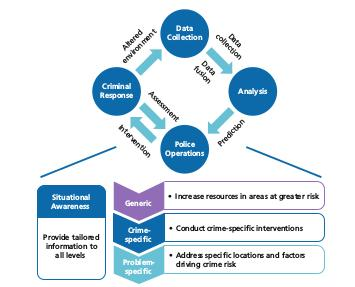
\includegraphics[scale=0.7]{prediction_process}
    \caption{Process of predictive analysis for crime prevention\cite[xviii]{PP13}.}\label{fig:ledprocess}
\end{figure}

Important sub-tasks need to be implemented between the main parts.\cite[13--15]{PP13} During data collection, it is also important to have data in adequate quality and easily processable format. Data need to be merged and aggregated. In the analytic part, it is necessary to focus on different methods for different predictions. As part of the police operations, a human factor is still needed to interpret the results of analyses and prediction to decide which interventions will be realised. In retrospect, it is also important to evaluate which interventions was successful and to examine why. According to the criminal response, it is still necessary to go back to the beginning of the process and to edit data to reflect the actual situation. It can be expected the criminality does not completely disappear, but for example, it moves somewhere else or just temporarily decrease.

Use of predictive analysis is not only an implementation of a new system. With the introduction of a predictive system is related the maintenance and access to historical data in the correct format, the training of the police patrol staff, also the training of the officers, correct use of all available tools and technologies, etc. The main benefits of introducing new predictive system include reducing crime, reducing the number of victims of crime in risk areas, more efficient planning of police patrols (saving time during planning strategies or the correct layout of the places where patrols are moving), but also increasing public confidence in the work of the police.\cite[290--294]{futuremaps} 

\section{A taxonomy of predictive methods}

With regard to how extensive the police activities are, it is not possible to assume, that there is a universal predictive method for all types of criminality. In this section, the basic division of methods of crime prediction is described. 

There are four main groups of predictive methods, which are defined based on specialising in the domain (for example risk areas, offenders or victims) and how data are handled (whether a small amount of data and simple methods, or big data and advanced methods)\cite[8--12]{PP13}:

\begin{enumerate}
    \item Methods for prediction crime -- predictions in which place and time the crime likely occurs.
        \begin{itemize}
            \item \textit{Data}: historical crime data when and where the crime or offence occurred, further additional data such as who and how the crime reported, geographic data, socio-demographic data, etc.
            \item \textit{Methods with a small amount of data}: Hot-spot analysis, basic regression models, Heat maps, derivation of dependencies between the environment and the most risk areas. 
            \item \textit{Methods with big data}: advanced Hot-spot analysis, Risk Terrain analysis, Near-repeat analysis, Spatio-temporal analysis, Regression analysis, Classification, Clustering,  etc. 
        \end{itemize}
    \item Methods for predicting offenders -- predictions aimed at identifying individuals as potential offenders.
        \begin{itemize}
            \item \textit{Data}: data about individuals, their activity over time and links to other people.
            \item \textit{Methods with a small amount of data}: manual search of suspected people, clinical instruments to summarise the generally known risk properties of people, etc.
            \item \textit{Methods with big data}: Near-repeat analysis, Regression analysis, Classification, etc.
        \end{itemize}
    \item Methods for predicting perpetrators' identities -- predictive techniques based on comparisons of profiles of various perpetrators and their crime history.
        \begin{itemize}
            \item \textit{Data}: personal data of perpetrators and their crime history, links between perpetrators, recorded movement of perpetrators by \gls{gps} tracking, etc.
            \item \textit{Methods with a small amount of data}: manual search of all materials and drawing inferences, crime linking, location areas both near and between crimes in series, manual requests and review of sensor data.
            \item \textit{Methods with big data}: computer-assisted queries and analysis of intelligence, sensor and other databases, statistical modelling to perform crime-linking, analysis using geographic profiling tools.
        \end{itemize}
    \item Methods for predicting victims of crimes -- predictions aimed at groups or individuals likely become victims of crime.
        \begin{itemize}
            \item \textit{Data}: socio-economic data, geographic data, historical personal data about offenders and victims, etc.
            \item \textit{Methods with a small amount of data}: Hot-spot analysis, manual review of reports, graph and maps of most frequent crime sites and identifying people most likely to be at these locations, manual review of domestic disturbance incidents, etc.
            \item \textit{Methods with big data}: advanced Hot-spot analysis, Risk Terrain analysis, advanced data-mining techniques used local and another accessible crime database, computer-assisted databases to identify domestic and other disturbances, etc.
        \end{itemize}
\end{enumerate}

Also, time is an important factor for crime prediction. Therefore the predictive methods differ according to whether they are short-term (immediate future, day or few days ahead), medium-term (near future, weeks or months ahead) and long-term (distant future, quarter or years)\cite[42]{Chainey2015maps}. Figure~\ref{fig:chainey_time} shows the timeline and specific types of prediction. For example, it is recommended to use Repeat and Near-Repeated analysis for short-term predictions, Hot-spot analysis for medium-term predictions and Spatiotemporal Regression analysis for long-term predictions.

\begin{figure}[ht]\centering
    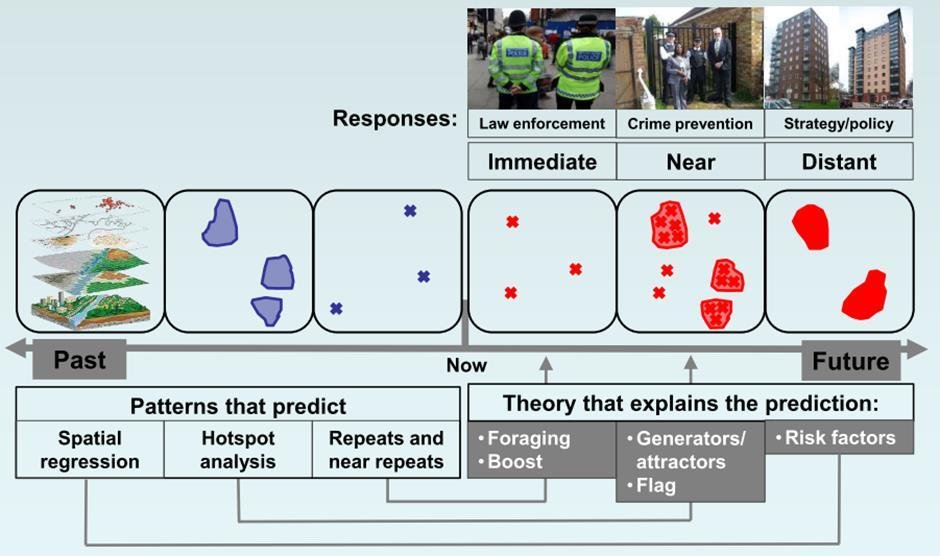
\includegraphics[scale=0.33]{chainey_time}
    \caption{Process of predictive analysis for crime prevention\cite[39]{Chainey2015maps}.}\label{fig:chainey_time}
\end{figure}

\section{Methods for predicting crime}

As mentioned before, the methods for predicting crime have been examined for a long time, and therefore different approaches were developed. Classification of these methods into individual categories is not strictly defined, and for example, some of the approaches can combine more methods from the different domain.   

This thesis is focused only on \textit{Methods for predicting crime} where the historical crime data can be used. The data have to include the determination of the time and location (ideally by \gls{gps} coordinates) of each crime. The objective of methods is to predict in which place and time the next crime likely will occur. In this section, the main methods from this category are briefly introduced. 

\subsection{Hot-spot analysis}

Methods based on Hot-spot use fact, that data are not uniformly distributed in the space and time. Therefore at different places in a different time, the frequency of crime is low and others high. The basic assumption of prediction is that crime likely occurs where it occurred repeatedly in past. The result of Hot-spot analysis is the identification of the most endangered points on the map (hot spots), where crime is often repeated. \cite[19]{PP13}

The area for prediction is a basis. The map of this area has to be on a scale for that predictions are relevant. The data are aggregated into small units (for example squares with edge size 100 metres) and their size can greatly affect the result prediction. If the units are too small, some important areas may be omitted (information is broken down). On the other hand, if the units are too large, the information collapses and the allocation of police patrols is not easy. The four basic methods for creating hot-spot map exist\cite[19--29]{PP13}:

\begin{itemize}
\item \textit{Covering Ellipses} -- Simple algorithm which finds large clusters of crime and creates the most appropriate ellipse over them to optimise a size of covering an area. This algorithm is easy to implement, but the big disadvantage is that ellipses cover large areas where often nothing happen.

\item \textit{Single and Dual \gls{kde}} --  The main goal of Kernel density estimations is to decompose crime points into a continuous function -- interpolation of this function, based on the distance of each crime from others. It is possible to use kernel function -- normalised weighted function in which the data points are smoothed into the continuous function. The user selects one of the defined kernel functions and the bandwidth, and for each crime, it calculates the core function. Therefore each crime is central to the core function and other crimes located in the defined area are weighted according to the core function. Overlapping areas of kernel functions are stacked so that it creates the hot spot in places where it the most overlays. Single \gls{kde} uses only crime data, Dual \gls{kde} also uses additional data for example movement of people in given areas. The values of the final kernel function are projected into the map using a colour scale. Too much bandwidth of kernel creates a too general function and few very significant hot spots, on the contrary, small bandwidth creates many separate and insignificant hot spots. In the figure \ref{fig:hotspot} is example of difference between Single and Dual \gls{kde}.

\begin{figure}[ht]\centering
    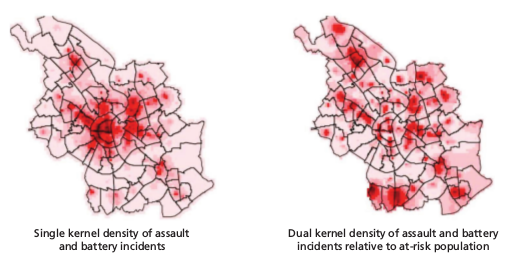
\includegraphics[scale=0.5]{kde}
    \caption{Examples of Hot-spot mapping in Cologne city in Germany. In the first image the Single \gls{kde} is used, the second image shows Dual \gls{kde}.\cite[25]{PP13}}\label{fig:hotspot}
\end{figure}

\item \textit{Quadrat thematic mapping} -- This method aggregate data into the grid -- into the same large squares or polygons. Individual squares are coloured according to defined rules. It also depends on the scale of map and type of crime. It is also called Heat mapping. This method is simple but the disadvantage is that the scale has to be selected to reflect the type of data and then the resulting hot spots are significantly affected by this option. 

\item \textit{Jurisdiction-bounded areas} -- The basis is the aggregated data into a thematic map, which is composed of different polygons according to the jurisdictional geography (for example police districts). As the Quadrat thematic mapping method, the data are aggregated and coloured according to these polygons. This method has the same disadvantage as the Quadrat thematic mapping, and it is also sensible to select a correct scale for colouring. Also, the polygons are usually too big to find adequate risk areas. 
\end{itemize}

In general, the Hot-spot mapping can be a useful tool for medium-term and long-term predictions. Chainey explored that some types of crime are significantly repeated in most of the hot spots every month\cite[38]{Chainey2015maps}. For example, in Newcastle city (United Kingdom) there were 68 \% of thefts from the person and 25 \% of theft from a vehicle in the same hot spots as the month before. There is the example a Hot Spot Analysis using crime data in the figure~\ref{fig:hotspot}. 

\subsection{Repeat and Near-repeat analysis}

Repeat victimisation is an empirically observed process where a person or other object (for example a building) is repeatedly a victim or a target of a crime. This is also related to the near-repeat victimisation process, where people or objects near a recent incident are also at increased risk of victimisation. These repetitive formulas have been identified for several types of crimes - robberies, theft of vehicles and shooting.\cite{Chainey2016repeat} Chainey defined two main theories why repeat and near-repeat victimisation occurs\cite{Chainey2016repeat}:

\begin{itemize}
\item \textit{Boost account theory} -- It assumes that the perpetrator decides to return to the site of the previous crime by boosted previous success and information about the site or victim. This also applies to near-repeat victimisation, where the perpetrator is familiar with the environment and assumes that it will be a similarly demanding crime to do (for example, when a perpetrator knows the neighbourhood, if the houses are similarly constructed, etc.). Optimal nutrition theory explains why boost account theory is in practice. This approach compares perpetrators to animals looking for food. The perpetrator must consider what is better for him, whether to return to the same crime scene, where he already knows it and knows how to commit the crime or to make a major effort to find a place. If it is inappropriate to repeat criminal activity in the area, the offender moves elsewhere.
\item \textit{Flag account theory} -- This theory is based on the fact that an object or person is repeatedly the target of various offenders because they show signs of availability (for example, the building is repeatedly not adequately secured and the burglary is easy, or the victims repeatedly occurs in places, where are easily attackable).\cite{Chainey2016repeat}
\end{itemize}

In practice, these phenomena often occur concurrently. For example, an easy target is repeatedly attacked by a single perpetrator for a short period of time and another perpetrator appears after a random time. Several approaches exist to predicting repeat and near-repeat victimisation.\cite{Short2009repeat} In the case of small amount of data, local knowledge and familiarity with crime in the surrounding area can be used. For large data, it is advisable to use sophisticated methods, for example, modelling situation using random processes. The goal is to model a random process for each object or person. With a given probability the model evaluates the likelihood of further repetition of the crime. The example of Near-repeat prediction is in the figure~\ref{fig:nearrepeat}

\begin{figure}[ht]\centering
    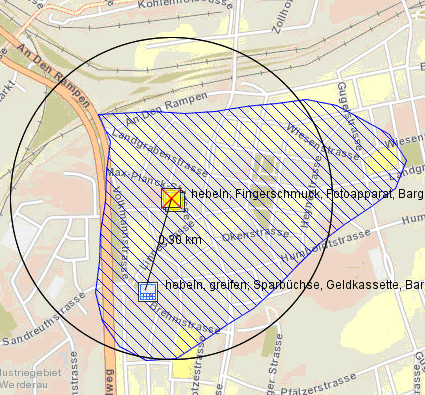
\includegraphics[scale=0.4]{nearrepeat}
    \caption{Examples of Near-repeat prediction.\cite{nearepeat_image}}\label{fig:nearrepeat}
\end{figure}

\subsection{Spatio-temporal Analysis}

Spatiotemporal Analysis is based on the investigation of the relationship between crime and the environment where crime occurs. The goal is to predict where the crime will occur in the future, based on a combination of information about the environment and crime history. Important in this analysis is to have a large amount of external data such as weather data, data about irregular events, points of interest (restaurants, shops, bars, etc.), socio-demographic data (population, age distribution, employment in given sub-areas, etc.). Data is transformed into so-called features, so the same flags with different values are processed for each defined area (squares or polygons).\cite[44--45]{PP13}

Dependencies between the studied features in a given area are explored using basic statistics (for example by means of average or standard deviations) or by using more complex mathematical models (for example Spatial Linear Regression or Clustering). The only one area during a time period (time series) can be investigated within Spatio-temporal Analysis. It is also possible to compare the number of crimes in different months, years, etc. It is also possible to separate time series into different components and to find seasonality or pattern.\cite[48--49]{PP13}

Using a temperature table (sometimes also referred to as Heat Map), it is also possible to see how the number of crimes in a specific territory is changing over time (not in the graph, but in the table). Often, the table is created that the columns contain for example days of the week and in rows there are hours. The individual cells of the table are aggregated by a number of crimes, and they are differentiated using a colour scale. It is easy to examine and compare how criminality changes in the individual cells observed, and for example to reveal the times and days of the most crimes and how different it is for different types of crimes.\cite[46--47]{PP13} Example of a time series and a Heat Map is in the figure~\ref{fig:temporal}

\begin{figure}[ht]\centering
    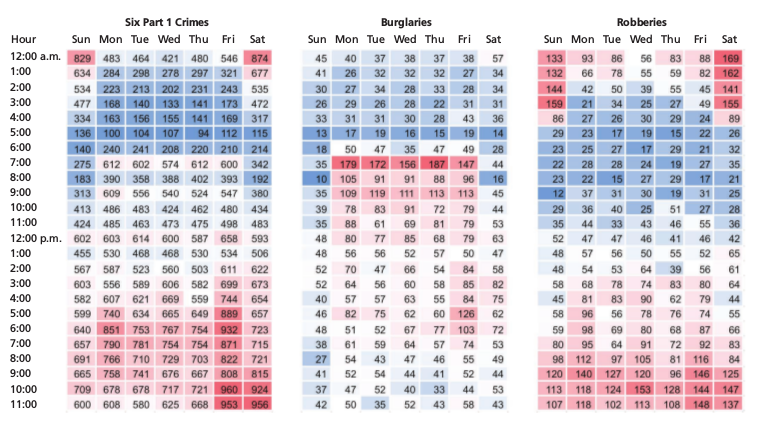
\includegraphics[scale=0.4]{heattable}
    \caption{Example of a temperature tables of crimes, burglaries and robberies in Washingthon D.C in the United Sates.\cite[47]{PP13}}\label{fig:temporal}
\end{figure}

\subsection{Risk Terrain Analysis}

The outcome of Risk Terrain Analysis is, as with Hot Spot, the identification of potentially dangerous places. However, the Risk Terrain Analysis is not based on the clustering of historical crimes, but the objective is to identify the geographic elements (points of interest) that contribute to crime (for example bars, alcohol stores, etc.).\cite[50]{PP13}

The advantage of this method is that it uses not only historical data on crime but also additional information on places where crime is repeated. Compared to the Hot Spot Analysis, therefore, it can show the causes of the crime. However, many risk factors can be related to more populous areas rather than the risk points so that it has to be taken account when this method is used. 

A simple heuristic method is Risk Terrain Mapping.\cite[51]{PP13} It is based on interleaving several layers of interest points with a layer of crimes over a certain period of time using \gls{gis} tool. These layers are projected into a user-defined grid, and the risk areas (most often squares) are those, where the most risk points are found along with the crimes. The grid can be coloured using a colour scale so that the areas are different shades based on probably risk.

A statistical approach to Risk Terrain Analysis\cite[52]{PP13} consists of two phases of the calculation. In the first stage, the distances between the crimes and the various risk points are compared and saved. In the second phase, the monitored area is divided into a grid and for each polygon (again most often squares) is calculated how they are similar to each other regarding distances from risk points. Then the grid can be also coloured. Example of the output of Risk Terrain Analysis is in the figure~\ref{fig:rta}

\vspace*{0.5cm}
\begin{figure}[ht]\centering
    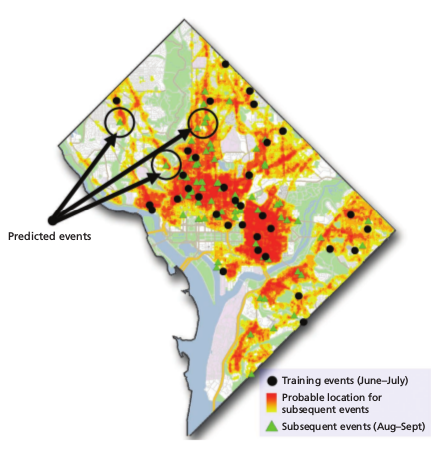
\includegraphics[scale=0.5]{rta}
    \caption{Example of the output of Risk Terrain Analysis based on data on purse snatchings in Washington D.\,C. summer 2008.\cite[54]{PP13}}\label{fig:rta}
\end{figure}

\subsection{Data mining}\label{sec:datamining}

Data mining is a process of building a mathematical model to make a prediction based on preprocessed input data. Basically, it is practice of searching through large amounts of data to find pattern and trends or potentially useful and for human hidden information.\cite[33--34]{PP13} The whole process have several phases according to the \gls{crisp} standard -- business understanding, data understanding, data preprocessing, data modelling, evaluation and deployment.\cite[10]{Chapman2000crisp} The schema of this process is in the figure~\ref{fig:crisp}.

\begin{figure}[ht]\centering
    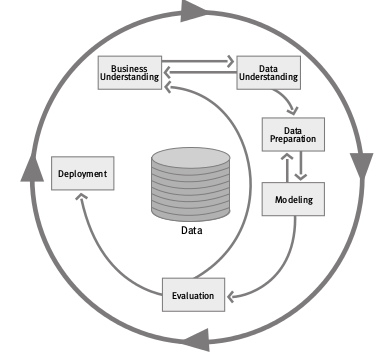
\includegraphics[scale=0.6]{crisp}
    \caption{Schema of the \gls{crisp} process.\cite[4]{Chapman2000crisp}}\label{fig:crisp}
\end{figure}

It can be observed that the \gls{crisp} is similar to the process of predictive analysis for crime prevention, which was mentioned in the section~\ref{sec:methodology} and in the figure~\ref{fig:ledprocess}. It can be assumed that this process is inspired by the \gls{crisp} process. 

At the beginning, it is crucial to understand the data and set the main objectives of the analysis. During data preprocessing it is important not only to clean and prepare data into a suitable format but also to select relevant and non-redundant data, extract new data or sample data if it is necessary. 

During data modelling, many of algorithms can be used to create predictions, so that some of them have to be selected and their performance has to be verified. A model can consist of only one simple method, or it can be more complex and sophisticated. In order to select a good model, in most of the cases, data analysts have to understand and analyse individual methods and algorithms and select the best one. Consequently, they should be able to optimise the model on input data to be as good as possible with data, on which model was not trained. 

Methods and algorithms used in data mining are based on statistics, optimisation and machine learning approaches. Machine learning is, in general, the learning of knowledge and patterns from input data or suggestions. Machine learning is based on the same principle as human learning -- from examples and experiences represented in the form of data, they learn patterns and can optimise their results based on the defined error. These methods are defined for example as a general function and can be applied to a plenty of tasks, including predictions of crime. Depending on the type of input data and learning approach, machine learning is divided into three basic areas: 

\begin{itemize}

\item \textit{Supervised learning} -- It is necessary to have the input data even with their expected outputs (labelled data). The target data are 'teacher' and so that the model is optimised to generate output as similar to real output as possible.\cite[xii]{Hastie2001statisticallearning} However, the goal is not to find precisely projection from input data into target data, but to find approximation which is generic and produce correct output also for new incoming data. Based on a type of target data, in general, two approaches exist -- regression (targets are real numbers, and the goal is to approximate these number) and classification (targets are categories or classes, and the goal is to classify input data into correct classes). In practice with real data, the complex problem have to be solved, for example, intersect or separate in many dimensions, which can be visualised well for humans. There are many different methods, which can be used, for example, Support Vector Machines, Naive Bayes, Decision Trees, Neural Networks, etc.

\item \textit{Unsupervised learning} -- If the target data is not available, the clustering method can be used for finding some clusters or dependencies in data.\cite[xii]{Hastie2001statisticallearning} Clustering is based on the determination of the similarity of individual data records (for example using metrics such as Euclidean distance), and using this similarity data are separated or clustered into clusters. The most well-known clustering algorithms include Hierarchical clustering, Nearest Neighbours, K-means, Self-organizing Maps, etc.

\item \textit{Reinforcement learning} -- This learning approach is based on the insertion of an agent (or multiple agents) into a foreign environment, and the agent is learned using feedback from this environment to bring as much profit as possible.\cite[4]{Sutton1998reinforcement} Feedback can be both positive and negative. Different types of agents are defined -- an agent with requests (the agent learns the benefit function for the states),  Q-learning agent (the agent learns the action based on the expected utility), reflection agent (the agent learns the strategy to use the action for the given condition). Also, different types of learning are  -- passive (the agent works with a predefined strategy) and active (the agent does not have a firm strategy, he learns what to do, for example from exploration environment). 

\end{itemize}

The learning and model building can also be different. The problem is optimisation task which can be solved for example by gradient methods, evolutionary algorithms, combining the models, searching in state space, etc. 

After the model building, the evaluation phase is important -- how successful the model is and how it can be generalised. The performance of the model can also be verified by many methods, for example by testing on the part of data which the model does not use during training. The final phase of the whole \gls{crisp} process is to deploy the final model into production and to maintain the entire system.

\section{Software available}\label{software}

In 2017, a several well-functioning and police-proven predictive tools are available. They use both spatial and temporal information from data and many other factors influencing criminality. In most of the cases, these tools are based on \gls{gis} framework and allow to use various models to predict crime. The success of prediction fundamentally depends on the environment, type of the offence and data quality. It must be taken into account that often occurring crimes (such as thefts from a vehicle) are much better predicted than crimes such as rapes, murders or assaults.  

\subsection{PredPol}

The most popular software for crime prediction is cloud-based technology PredPol.\cite{predpol} It was developed in 2012 in the United States, and the final product is the result of 70 years long research between the Los Angeles Police Department and University of California, Los Angeles. 

They evaluate a wide variety of data types and behavioural and forecasting models, but they do not specify which methods. For predictive analysis, they use only information about crime type, crime location date and time of a crime, no personal data about individuals eliminating any personal liberties and profiling concerns. It is not based on the Hot-spot analysis. They use ArcGIS as a \gls{gis} framework. The smallest unit, which can be examined, is a square with an edge size of 500 feet (approximately 150 meters). 
 
Many examples of crime reduction after the introduction of PredPol was noticed in the United States.\cite{predpol_result} In some territories, the reduction of crime rates by up to 30 \% (for example in the Alhambra, CA Police Department or Norcross, GA Police Department). 

\subsection{HunchLab and CrimeView Dashboard}

Competitive crime prediction software is HunchLab which was developed in the United States by Azavea company. The first version was deployed during 2008--2011 for Philadelphia Police Department and the Office of the U.S. Attorney. In 2014, the new version 2.0 was introduced.\cite{hunchlab} 

A predictive model is based on repetitive time patterns (day of the week, seasonal phenomena, etc.), weather, Risk Terrain Analysis, socio-de\-mo\-gra\-phics data, crime history and Near-repeat analysis. They are able to build model even from historical data. For model building, machine learning algorithms are used -- \gls{gbm} and AdaBoost. They also use ArcGIS as a \gls{gis} framework. The smallest unit, which can be examined, is a square with an edge size of 100 metres.  

HunchLab can be integrated as a predictive module into the CrimeView Dashboard visualisation and analytic tool. It was developed by The Omega Group in the United States. The predictive module from The Omega Group can also be used, however, it is based only on Near-repeat Analysis and Hot-spot Analysis.

\subsection{PRECOBS}

The popular software which was developed in Europe is PRECOBS.\cite{precobs} It was introduced in 2011 in Germany by the Institut für musterbasierte Prognosetechnik. 
A predictive model based on the history of crime and near-repeat analysis is only suitable for some types of acts (for example street robbery, armed robbery, theft of a motor vehicle). The predictions are based on Near-repeat analysis only with historical crime data no personal data. They used OpenStreetMap Maps as a \gls{gis} framework. 

They reported crime reduction up to 30 \% of a certain kind of crime after the software has been deployed.\cite{precobs_percent} The PRECOBS is used in several cities in Germany and Switzerland. 

\subsection{Hitachi Visualisation Predictive Crime Analytics}

In Japan, the Hitachi Data Systems Corporation also developed crime prediction software -- Hitachi Visualisation Predictive Crime Analytics.\cite{hds} It was introduced in 2015, and it is first predictive tools which process not only historical crime data, emergency call data, live weather radar data in real time but also uses data also from social media and Internet data. It can be combined with Hitachi Video Management Platform to process video information and improve predictions as well.

The predictions are based on multi-variable machine learning models. The units, which are examined, is a square with an edge size of 200 metres. The user can use different maps, for example, ESRI maps, Bing maps, OpenStreetMap, Google Maps. The system is used for example in Japan or the United States. 

\subsection{IBM -- SSPS Modeller}

IBM is not behind. In 2015, they presented crime prediction application IBM SPSS Crime Prediction Analytics Solution Service.\cite{ibm} It is not a black box solution, but it is necessary to create a solution in Modeler, or to manage the software and to construct your own model. IBM offers support and helps to find the right solution.  

The standard machine learning algorithm is implemented in SSPS Mode\-ler, such as Regression analysis, \gls{dt}, \gls{nn} etc. It can be connected with geographic analysis with ArcGIS. 

They reported violent crime and homicides reduction up to 30 \% using IBM Crime Insight and Prevention solution in the Richmond Police Department, Virginia over the 12-month period.\cite[4]{ibm_percent} 

\subsection{Other tools}

There are many other tools which provide various type of prediction from simple visualisation to complex statistic models. For example, Motorola company developed COMMANDCENTRAL Predictive\cite{motorola}, open source tool Cri\-me\-Stat\cite{crimestat} developed by Ned Levine in Texas, the tool for Risk Terrain Modelling RTMDx\cite{rtmdx} developed at The State University of New Jersey, open source tool for Near-repeat Analysis Near Repeat Calculator\cite{nearrepeat} developed at Temple University in Philadelphia, etc. 

%%%%%%%%%%%%%%%%%%%%%%%%%%%%%%%%%%%%%%%%%%%%%%%%%%%%%%% CHAPTER %%%%%%%%%%%%%%%%%%%%%%%%%%%%%%%%%%%%%%%%%%%%%%%%%%%%%%%
\chapter{Data preparation}\label{sec:data}

Before mining information from the data, it is necessary to have them in the suitable format for predictive analysis. Correctly processed data should significantly affect the result analysis. In this chapter, the parts of the \gls{crisp} process, which are related to data, are described  -- data understanding and preprocessing.

The \gls{crisp} model is a standard for data mining predictive methods and was described in the previous chapter in the section~\ref{sec:datamining}. However, the results and the recommendations related to data processing can be applied in the different domain, not only in data mining.  

\section{Business and data understanding}

The business and data understanding is key, but sometimes omitted part of \gls{crisp}. It is the first part of \gls{crisp}, and it could be crucial for other data manipulation. 

For preparing a quality analysis, it is important to understand what is demanded and which goals should be achieved. It is called the business understanding of data. In many cases, the analyst gets data and has the only one goal -- play with data and try to find something interesting. However, if the task is more complicated and requires a lot of working hours and finally placing in service, the business plan is obligatory. The main goals are defined reasons to make analysis, objectives to achieve, select the best methodology and create approximate timetable.\cite[14]{Chapman2000crisp}

Next phase is data understanding from the perspective of the data source. The main goal is to know from which sources data come, whenever the data are structured or not, and in which formats are provided. \cite[18]{Chapman2000crisp} The source could be a relational database (one or many tables) or a \gls{xml} database, exported data in \gls{csv}, \gls{txt} or \gls{xml} format, compressed data or for example logs from a system. If the data are unstructured, for example, extensive text files, images, the structure has to be defined. The most common structure is to separate data into rows (records) and columns (attributes). If the data contain images, audio or video records, the transformation into digital form has to be done. 

Another task is to look at data quality. Data may be inconsistent, contain illegals characters, or there could be some missing values. After removing invalid parts, the size of data could be insufficient, or the required information could be lost. This process is important to prevent problems in the next data processing parts.

Finally, the basic statistic can be computed, for example, mean of data, most common values, maximal or minimal value, etc. Together with data description, it gives the complete view of the source data. 

After this part of the process, the data are structured and valid. Analyst knows what the particular records mean (for example data description is available) and also knows, which requirements have to be accomplished. Also, the first insights into the data are discovered, or interesting subsets to form hypotheses for hidden information are detected.

\section{Data preprocessing}

Usually, the most comprehensive and time-consuming part of \gls{crisp} is data preprocessing. The goal is to prepare the final dataset from raw data for further analysis. This step is consists of three essential parts - data cleaning, data constructing and data selection.

\subsection{Data cleaning}

Data cleaning is process that raises the data quality to the level required by the selected analysis techniques.\cite[21]{Chapman2000crisp} Real data are not clean in general -- it means there are missing values, inconsistency, and various formats. Therefore, the data have to be repaired or removed, which can significantly increase the value of the data. 

Before data transformation, the selecting only relevant data is useful. For example, the data are combinations of a several tables and many of columns. Some of them are not interesting for analysis because they contain unnecessary information for the task, and selection only relevant data make the other preprocessing methods more efficient. 

Missing data could cause many problems, for example, some algorithm do not work with them.\cite[43]{Chapman2000crisp} The missing value could be expressed in many formats such as 'NAN', 'NULL', 'NA' or 'N/A', and there can also be combinations of these so that the first step is detection and unification of all missing values in data. The next step is to handle the records, where missing values are contained. Remove them is one possibility. Another approach is to replace missing values with neutral values, for example with zero or the average value computed from data. The last possibility is to replace the missing values using the algorithm, which recommends the possible value based on characteristics of other records (for example using clustering methods).

Similar problem could be inconsistency of data.\cite[43]{Chapman2000crisp} For example, a dataset contains column 'month', and there are values less than 1 or greater than 12. Also, the inconsistency between two columns can be detected. For example the dataset contains column 'gender' with values \{'men','women'\} and the column 'pregnant' with values \{'True', 'False'\} -- the combination \{'men', 'True'\} does not make sense. Finally, real data often contains a noise or outgoing records. This could be detected using statistical tests or advanced algorithm. If the dataset contains records with incorrect values in terms of data description or data properties, they should be repaired or removed. 

If data contains attributes with formatting, it could be unified too.\cite[43]{Chapman2000crisp} For example date and time attributes could have many formats such as text format (for example 'YYYY/mm/dd' or 'dd-mm-YYYY') or number format (for example Unix Timestamp). Since the data are in the unified format, they can be modified or separated later in the data preprocessing.

The output of this transformation is clean and consistent data. This process can improve the quality of analysis as well as speed up calculations. 

\subsection{Data constructing}

This task is about constructing new data according to properties of the original dataset. The attributes could be for example separated, derived, aggregated or transformed to have better properties from the perspective of mathematics and statistic. 

\subsubsection{Data categorisation and parsing}

Most of the algorithm operate just with numerical values of data and only with maximum defined values per attribute. Either data mining tools can handle it automatically, or it can be done manually. If the attribute are composed of separable parts, parsing is also useful.\cite[44]{Chapman2000crisp}

Conversion of data from non-numerical values to numerical is easy -- the mapping between text representation to number representation is used. For the algorithm, the numbers are used and then for result presentation the values are converted back. The problem is when the attribute consists mostly of unique values. Then the categorization is necessary. The attribute is divided into groups or categories according to distribution of values.\cite[45]{Chapman2000crisp}

The one-hot encoded form of data can be useful.\cite[45]{Chapman2000crisp} One-hot encoding is the transformation from category attribute into space of attributes which are represented by values 0 or 1. For example, if an attribute is 'animal' and the categories are 'turtle', 'polecat', and 'honey badger' than the new attributes are 'animal turtle', 'animal polecat', 'animal honey badger'. If the category of record is 'turtle', after encoding the value of attribute 'animal turtle' is 1 and 0 in the case of attribute 'polecat' and 'animal honey badger'. There are a lot of other encoding methods, especially for text attribute preprocessing where whole sentences could be encoded into vectors, but their descriptions are out of the scope of this thesis.

Finally, some type attributes can be separated.\cite[45]{Chapman2000crisp} For example, attributes which hold information about date and time. Convert the date and time into numeric values is easy because every date and time have unique number format (for example Unix time stamp). However, this format can destroy useful information and context of the date or time. The better interpretation is separate date into new attributes by the component such as day, month, year, etc. It can improve analysis and help to find an interesting connection in data. 

There are many other possibilities how data derive, aggregate or encode and then improve data quality. Nevertheless, it can also enter deficiency into data, for example, redundancy and correlation between attributes or enlarge the dataset considerably.

\subsubsection{Data extraction}

Data can be also created using properties of individual attributes or combination of them. It usually depends on creativity and fantasy of analyst.

For example from data, where an attribute is a date or time, time series (history) can be derived. Alternatively, if the data contains geographical information, the new attributes about locality can be discovered. From text's attribute can be mine sentiment, context or other interesting attributes. From image data, new information can be segmented using image processing techniques. 

Data can also be preprocessed and transformed using methods which are primarily developed for predictive analysis such as \gls{nn} or \gls{rf} (more about the predictive methods is in the chapter~\ref{sec:analysis}). For example \gls{cnn} (see section~\ref{sec:cnn}) could be used for extract new attributes from images or from signals. The \gls{cnn} is trained with original image or signal data and then the parts of the net (corresponding part of filters -- hypercolumns) are used as new attributes.\cite{Perone2016hypercolumns} 

\section{Data reduction}

In cases where the dataset is huge, data reduction is recommended. Not always the rule 'the more information, the better' hold true in data mining. Due to large space of attributes, the computing can take a long time. Another reason is the prevention of overfitting models. Data could be noisy and redundant, and therefore the model is learnt by noise rather than general information.\cite[43]{Chapman2000crisp} For this part of data preprocessing is assumed that data are consist of a set of explanatory attributes and one response attribute. 

There are two possibilities how to reduce the amount of data. First, sophisticated methods for selection most important attributes (features) is called feature selection. Another method transforms the data into different space of attribute which is usually smaller and holds the same information. 

Because methods for data reduction could be complex, detailed description their algorithm is out of the scope of this thesis. So that I just briefly introduce base principal some of them.

\subsection{Feature selection}

From analyst point of view, all features are equally important, but from the perspective of mathematics and statistic, some features are more important than the others. The statistic methods are able to compare values of all features and discover for example duplicity, correlation or other undesirable occurrences in data. After that, useless features can be removed from the dataset. 

By using univariate selection, each single feature relationship with the response feature can be evaluated individually. Many methods for comparing two variables can be used from statistics. One of the simplest methods is Pearson correlation coefficient, which measures a linear correlation between two variables. \cite{Saabas2014univariate}  The result is a value from -1 to 1, where -1 and 1 mean perfect correlation (negative -- one variable increases, the other decreases or positive -- the both are the same) and 0 means no linear correlation. Pearson coefficient is the ratio between covariance ($cov(X,Y)$) of two variable and product of their standard deviations ($\sigma_X$, $\sigma_Y$).

Another approach is a comparison of all explanatory features together. Simple machine learning algorithm such as linear regression or \gls{rf} can be used.\cite{Saabas2014regularization} 

By using linear regression, the feature importance is measured as weights ($w_i$) from optimal weighted linear combination of explanatory features ($x_i$) and some noise $b$ (or $b = 1 w_0$) against response feature ($y$). The definition of problem is:

\begin{equation}
\mathbf{y} = \mathbf{x_1} w_1 + \mathbf{x_2} w_2 + \cdots + \mathbf{x_n} + w_n + \mathbf{b} \text{ or } \mathbf{y} = \sum_{i = 1}^{N}{\mathbf{x_i} w_i} + \mathbf{b} 
\end{equation}

\noindent The optimal weights are computed by optimization of the defined loss function (for example $L(y, \hat{y}) = (y-\hat{y})^2$ -- mean squared error) over the all records. Then the optimal weights are values from -1 to 1 and the value -1 or 1 means the feature is important, 0 means the feature is not important. However, this approach is well suited for problems, where exist a purely linear relationship between features and response value. If the problem is more complex, this method is unstable -- small changes in the data cause large changes in the problem.\cite{Saabas2014regularization}

To get a more stable result, some regularisation techniques can be used with linear regression -- L1 or L2 regularisation. Both of them add penalty (value from 0 to 1) of weights into loss function, so after optimisation, the result weights are more stable. L1 add penalty $\lambda_1$ to all non-zero weights ($\lambda_1 \sum_{i = 1}^{N}{|w_i|}$), it means the weights which values are near 0, will became 0. This is also unstable, however, it is able to detect strong features. L2 adds different penalty $\lambda_2$ to all non-zero weights ($\lambda_2 \sum_{i = 1}^{N}{w_i^2}$), which means that it forces the coefficient values to be spread out more equally, and the resulting importance of features are more stable. \cite{Saabas2014regularization}

Finally, the \gls{rf} algorithm can generate feature importance. The \gls{rf} model is composed of a number of\gls{dt}s. Every decision tree is built a node by a node using features data and measure called impurity. The data are split into two nodes based on measure, one feature and response value, where the minimum impurity is achieved. (The detailed description of the algorithm is in the section~\ref{sec:rf}). Thus during training a tree, it can be computed how much each feature decreases the weighted impurity in a tree.\cite{Saabas2014rf} For a forest, the value from each feature is averaged and the result feature importance is based on this measurement. 

Regression or \gls{rf} can be also used in method called \gls{rfe}. The algorithm is based on repeated construction of a model and then choosing the worst or the best-scored features. The process is repeated until all features in the dataset are eliminated. Then the final features ranking is based on the evaluation in which iteration the each feature was eliminated. This method depends on the type of model, for example, unstable regression without regularisation should not be used, if the data are complex and correlated.\cite{Saabas2014all} 

Every method for feature selection has advantages and disadvantages, and mainly depends on data which is the best. The combination of them can provide better ranking than using only one of them.

\subsection{Data transformation}

For data reduction transformation of features into smaller feature space can be used. Two of the most popular techniques for this purpose are -- \gls{pca} and \gls{lda}.\cite{Martinez2001pcalda} These methods are used mainly in image recognition but also can be used for preprocessing. 

\gls{pca} is the orthogonal transformation from a set of possibly correlated variables into a set of linearly uncorrelated variables (principal components). The new space is matrix $W$ where columns are eigenvalues obtained by solving eigenstructure decomposition from the original data.\cite{Martinez2001pcalda} The result is that the first principal component has the largest variance possible. In fact, that it is orthogonal to the preceding components. The number of final components is the same or less than a number of features. The first component is from the point of view of \gls{pca} the best and the last is the worst. Therefore, the worst components can be removed from the dataset with minimal information loss. 

The similar method is \gls{lda} but use different space transformation\cite{Martinez2001pcalda}. The \gls{lda} creates a linear combination of variables which yields the largest mean differences between the desired classes. The goal is to maximise the between-class measure while minimising the within-class measure. Then find the best transformation, where a maximal ratio of these two measures is optimised. Finally, the new projection of data is found, and the feature can be selected.

There has been a trend to prefer \gls{lda} over \gls{pca}.\gls{pca} It is because the \gls{lda} deals directly with discrimination between classes, whereas the \gls{pca} deals with the data in its entirety for the principal components analysis without paying any particular attention to the underlying class structure.\cite{Martinez2001pcalda} However, the result of both also depends on the data. In some cases the \gls{lda} or \gls{pca} can obtain a better result, in the other cases, the result could be similar. 

To sum up the \gls{pca} and \gls{lda} can dramatically reduce feature space. Also, the new result projection of the data could better separate features in defined space so that it can improve prediction result.

\section{Resulting data format}

Usually, the result data are in the form of \gls{csv} (or it could be preprocessed images or signals). The data consist of only relevant information for further analysis, are cleaned and can contain new features derived from original data.

It is useful to check if the new data are correct and some error is not put into during preprocessing. Also, some basic statistic could be evaluated again. All changes which were made with original data should be reported. After all preprocessing steps, the result dataset is prepared for predictive analysis.  

%%%%%%%%%%%%%%%%%%%%%%%%%%%%%%%%%%%%%%%%%%%%%%%%%%%%%%% CHAPTER %%%%%%%%%%%%%%%%%%%%%%%%%%%%%%%%%%%%%%%%%%%%%%%%%%%%%%%

\chapter{Predictive modelling using Supervised learning}\label{sec:analysis}

Machine earning and Artificial Intelligence are concepts which evoke many emotions. Many people are afraid of Artificial intelligence and have different ideas about how algorithms work. For example, they imagine that the computers are thinking on their own and that the development in the field of artificial intelligence leads to machines which will take control of the world. For example, in the field of criminality prediction, some people imagine a predictive analysis as a divination with a crystal ball. 

The predictive methods described in this chapter give an overview of the current frequently used methods in the field of machine learning. These methods do not teach a computer to think independently, but they use mathematics and statistic to get as much information as possible from the given data. People are not able to evaluate so much information as computers are. For example, there could be millions of combination of values in the data, and people are not able to store this information in the memory, let alone evaluate them.

In this thesis, the main emphasis is put on predictive analysis using supervised learning, especially classification. Then several predictive methods were described more in detail -- methods based on neural networks and decision trees. Finally, some techniques find the best model configuration were introduced. 

Supervised earning methods were studied in connection to criminality prediction in the past. In 1998, Olligschlaeger \cite{Olligschlaeger1998prediction} proposed artificial neural network to predict emergency calls based on historical data from Pittsburgh DMAP system. In 2012, Wang \cite{Wang2012prediction} predicted crime based on spatiotemporal data and Twitter posts data. In 2013, Bernica \cite{Bernica2013prediction} used Generalised Linear Model to predict military conflicts of the United States with other countries based on historical and geospatial data. In 2015, Almanie \cite{Almanie2015prediction} used Apriori, Naive Bayes and Decision tree algorithm to predict crime based on data from Denver and Los Angeles. In 2016 Kaggle \cite{kaggle} (web community of data scientist) announced a competition to classify crime with historical data from San Francisco and a lot of competitors submit successful solution based mostly on machine learning algorithms, for example, Abouelnaga \cite{Abouelnaga2016prediction} used Gradient Boosting Machines, Decision trees, Naive Bayes and Random Forest algorithm.

\section{Classification}

Classification is a separation of the observed data into disjunct sets in general. There are two main approaches to classification based on a type of data. First, data are given as a set of observations with the aim of establishing the existence of classes or clusters in the data. This method is called clustering or unsupervised learning. Alternatively, the data consist of many classes, and the aim is to establish a rule how to classify a new observation into one of the existing classes. This method is called supervised learning.\cite[14]{Michie94machinelearning} In this thesis, I focused on supervised learning, and when the classification term is used, I mean a supervised learning approach. 

\subsection{Definition of classification}\label{sec:definitions}

From a formal view, classification is task, where the observed data $\mathcal{X}$ are able to cover finite number of disjunct classes,

\begin{equation}\label{eq:classification}
\mathcal{X} \subset C_1 \cup \cdots \cup C_m \land C_i \cap C_j = \emptyset \text{ for } i \neq j
\end{equation}

\noindent and based on finite number of data $(x^{(1)}, \cdots, x^{(p)})$ with known $C_1, \cdots, C_m$ classes, a classifier is constructed as a projection $f$ which classify every $x \in \mathcal{X}, f: \mathcal{X} \rightarrow \mathcal{Y}$, where $\mathcal{Y}$ is set of elements which indicates classes $C_1, \cdots, C_m$. \cite[6-8]{Bradley1999datamining}

A classification is binary, if there are defined only two classes -- $m = 2$ and the classes are $C_1 \text{ and } C_2$. Then $\mathcal{Y} = \lbrace0, 1\rbrace$ and for example $f(x) = 0$ means that $f$ classify $x$ into class $C_1$. A majority of models return $\mathcal{Y} = \Re$  or $\mathcal{Y} = [0, 1]$ (for example in form of conditional probability $\mathcal{P}$ (for given data $x$ is $f(x) = \mathcal{P}(Y = 1| \mathbf{X} = x)$, where the observed data $\mathcal{X}$ are realisation of random vector $\mathbf{X}$ and the observation of classes $\mathcal{Y}$ is realisation of a Bernoulli random variable $Y$).\cite[2]{Buja2005lossfunc} Therefore a threshold function $T(y)$ for division of data into two classes has to be defined. For example if $\mathcal{Y} = [0, 1]$, t = 0.5 and

\begin{equation}\label{eq:threshold}
T(y,t) =
  \begin{cases}
    0       & \quad \text{if } y \leq t\\
    1       & \quad \text{if } y > t\\
  \end{cases}
\end{equation}

\noindent then $f(x) \leq 0.5$ means that $f$ classifies into class $C_1$, and $f(x) > 0.5$ means that $f$ classifies into class $C_2$. 

\subsection{Supervised learning}

In many tasks with real-world data, there is not possible to find perfect classifier, which classifies all data into correct classes. In general, the problem is to find classifier $\hat{f}$ with optimal internal parameters $\hat{\theta}$, which predict the most likely value of $\mathcal{Y}$ given the other fields $\mathcal{X}$ over observed data (in which the target variable $\mathcal{Y}$ is given for each observation). 

To evaluate an error of the model $\hat{f}$ with parameters $\hat{\theta}$, a loss function has to be defined. The loss function compares each true class ($y$) with each estimated class ($\hat{y}$). There are many definitions of the loss function. Several examples are in the table~\ref{tab:loss_function}. 

\begin{table}[H]\centering
\begin{small}
    \caption{Examples of five loss functions for supervised learning task.}\label{tab:loss_function}
    \begin{tabular}{|l|c|}\hline
        Name & Function\tabularnewline \hline \hline
        0-1 loss & $L(y,\hat{y}) = \begin{cases} 0  & \quad \text{if } y = \hat{y}\\ 1 & \quad \text{if } y \neq \hat{y}\\\end{cases}$ \tabularnewline \hline
        L1 loss (Least Absolute Deviation) & $L(y,\hat{y}) = |y-\hat{y}|$ \tabularnewline \hline
        L2 loss (Least Square Error) & $L(y,\hat{y}) = {(y-\hat{y})}^2$ \tabularnewline \hline
        Hinge loss & $L(y,\hat{y}) = max{(0,1-y\hat{y})}$ \tabularnewline \hline
        Logarithmic loss (Cross-entropy) & $L(y,\hat{y}) = -y\log{(\hat{y})} + (y-1)\log{(1-\hat{y})}$ \tabularnewline \hline
    \end{tabular}
    \end{small}
\end{table}

By using the concept of a loss function, the goal of supervised learning can be described as finding a model $\hat{f}$ with $\theta$ minimising the risk $R(f) = \mathbf{E}\lbrace L(y, \hat{y}) \rbrace$, where the expectation $\mathbf{E} $ is over the joint distribution underlying the observed data and corresponding classes. This task is standard optimisation problem, which can be solved by methods for finding a minimum (for example using \gls{sgd}).\cite{theano_mlp} 

Usually, it is possible to construct a model which consists of complex functions which correctly classifies observed data. However, if the new data come to the input of model, the result classification is not good. The reason is that the classifier is learnt to the structure of observed data too much, and lost the ability to generalise on a new input. However, there are also cases when the less complex or perfect model is constructed and also not generalise well, because of observed data is finite and may be too small or corrupted by noise. In statistics, this is known as the bias-variance trade-off, and there are many techniques how to train model optimally.\cite[6]{Bradley1999datamining}

Even for that, the observed data are divided before training (it is called \gls{cv}). The simplest kind of \gls{cv} (holdout \gls{cv}) is to divide a model into training, validation and test subset\cite{Sheinder1997crossvalidation}. Often the training subset of data is the biggest (for example 70 \% from observed data), and validation and test subset of data are smaller (for example 20 \% a 10 \% from observed data). First, the model is trained on training data and during learning validate using validation data. After then the result accuracy and generalisation are measured on test data. 

Another technique $k$-fold \gls{cv} separates the observed data into several ($k$) subsets (not necessarily disjunct)\cite{Sheinder1997crossvalidation}. The methods consist of $k$ iterations, where training data contains $k-1$ subset, and the rest $1$ subset is used for testing. At the end, the average accuracy is computed. There is a possibility to take all data as training except one record and repeat until all records are as a testing record. It is called leave-one-out \gls{cv}\cite{Sheinder1997crossvalidation}. 

To summarise, first the model $f$ with $\theta$ has to be chosen, and data has to be prepared. Then, using observed data $\mathcal{X}$, the model is trained. Finally, the trained model $\hat{f}$ with an optimal internal parameter setting $\hat{\theta}$ is evaluated, and if it is good enough, it can be used for other predictions. The whole process of supervised learning is demonstrated in the figure~\ref{fig:supervised_learning}. 

\vspace*{0.5cm}

\begin{figure}[ht]\centering
    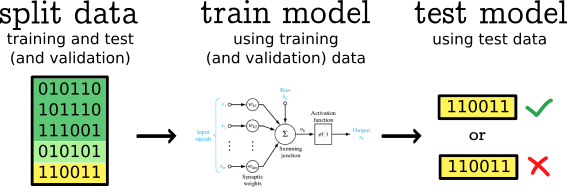
\includegraphics[scale=0.6]{sup_learn}
    \caption{Supervised learning process.}\label{fig:supervised_learning}
\end{figure}

\subsection{Binary classification evaluation}

There are many types of predictive methods which produce strong models for binary classification. It highly depends on data, which model to choose. An example of a model with two different test data problem is in the~\ref{fig:classification}. The good practice is to select a few common algorithms and to train several models. In order to compare which one is the best, many analyses and metrics can be used. 

\vspace*{0.5cm}
\begin{figure}[ht]\centering
    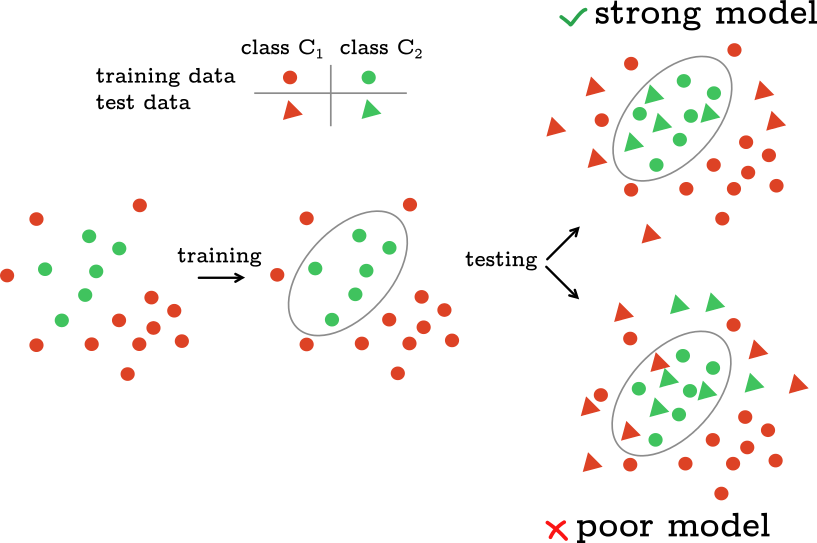
\includegraphics[scale=0.3]{class}
    \caption{Example of a trained model with two different test datasets.}\label{fig:classification}
\end{figure}

\subsection{Performance measures}\label{sec:measures}
For evaluation if the model is strong or not, the testing data, which were not seen a model during training, is usually used. If the model produce prediction in the form of class labels (negative '0' or positive '1'), the confusion matrix can be constructed. There are four main results in the confusion matrix -- \gls{tn}, \gls{tp} (correct or true classification) and \gls{fn}, \gls{fp} (incorrect or false classification).\cite[3]{Saito2015rocprc} The example of simple confusion matrix is in the figure~\ref{fig:cm}. In the figure~\ref{fig:cm_ev}, there is the example of confusion matrix constructed using the previous example of classification by the 'poor model' in the figure~\ref{fig:classification}.

\begin{figure}[ht]\centering
    
\includegraphics[scale=0.4]{cm}
    \caption{General confusion matrix for binary classification.}\label{fig:cm}
\end{figure}

\begin{figure}[ht]\centering
    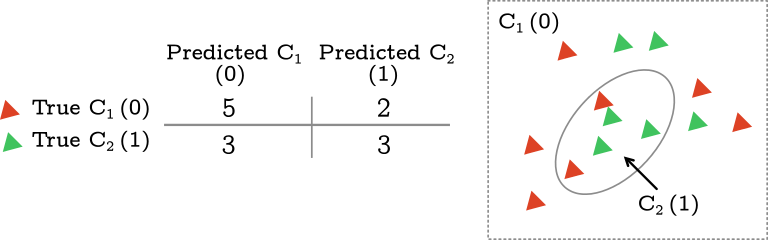
\includegraphics[scale=0.4]{cm_ev}
    \caption{Example of confusion matrix of the classification using 'poor model' from the figure~\ref{fig:classification}.}\label{fig:cm_ev}
\end{figure}

There are many evaluation measures of binary classification which are derived from the confusion matrix. The list the commonly used is in the table~\ref{tab:measures}.\cite[4]{Saito2015rocprc}

The most widely used measures is \gls{acc}.\cite[4]{Saito2015rocprc} The \gls{acc} is the proportion of all true predictions of classification. It is a number from 0 to 1, where 0 means no correct prediction and 1 means that all predictions are correct. The complement measure is \gls{err}.

{\renewcommand{\arraystretch}{1.7}%
\begin{table}[H]\centering
    \begin{small}
        \caption{Table of the most common measures of performance a classification.}\label{tab:measures}
        \begin{tabular}{|l|c|}\hline
    Measure & Formula \tabularnewline \hline \hline
        \gls{acc} & $\frac{(TP + TN)}{(TP + TN + FN + FP)}$ \tabularnewline \hline 
        \gls{err} & $\frac{(FP + FN)}{(TP + TN + FN + FP)}$\tabularnewline \hline
        \gls{tpr} & $\frac{TP}{TP+FN}$\tabularnewline \hline
        \gls{fpr} & $\frac{FP}{FP+TN}$\tabularnewline \hline
        \gls{tnr}& $\frac{TN}{FP+TN}$ \tabularnewline \hline
        \gls{fnr} & $\frac{FN}{FP+FN}$\tabularnewline \hline
        \gls{ppv} & $\frac{TP}{TP+FP}$\tabularnewline \hline
        \gls{npv} & $\frac{TN}{TN+FN}$\tabularnewline \hline
        Mathews correlation coeff. (MCC) & $\frac{(TP \times TN) - (FP \times FN)}{\sqrt{(TP + FP)\times(TP + FN)\times(TN + FP)\times(TN + FN)}}$\tabularnewline \hline
        \gls{f1} &  $2 \times \frac{PREC \times REC}{(PREC \times REC)}$ \tabularnewline \hline
        \end{tabular}
    \end{small}
\end{table}}

\gls{tpr}, also called \gls{sn} or \gls{rec} and \gls{tnr} also called \gls{sp} (the same as 1-\gls{fpr}) are also popular.\cite[4]{Saito2015rocprc} The \gls{tpr} is the proportion of true positive classification against all true classification. The \gls{tnr} is the proportion of true positive classification against all true classification. The \gls{ppv} also called \gls{prec} is also useful. It is proportion of correct predicted classes and all positives.

Interesting can be also combination of measures for example if the observed data are unbalanced. The \gls{mcc} ans \gls{f1} are useful for these cases.\cite[4]{Saito2015rocprc} The \gls{mcc} return value between -1 and +1. A value +1 represents a correct prediction, a value 0 means no better than random prediction and -1 indicates total incorrect prediction. The \gls{f1} can be interpreted as a weighted average of the \gls{prec} and \gls{rec}, where an a value 1 represent correct prediction and 0 indicates incorrect prediction. 

There are many measures and it depends on a problem definition and characteristic of data which measure is the best. It is useful to calculate more statistic and compare the results. 

\newpage
\subsubsection{Performance characteristic}\label{sec:roc}

There is also methods how to evaluate performance and find optimal threshold if the model produces prediction in the form of real numbers or probability. The methods are based on dividing the result prediction using all possible thresholds, calculate specific measures for each threshold, and plot the dependency graph. There are two basic methods -- \gls{roc} analysis and \gls{prc} analysis. \cite[4]{Saito2015rocprc}

The \gls{roc} plot shows the dependency between \gls{sp} and \gls{sn}. The resulting curve starts from (0,0) position and ends at (1,1) position. The baseline is a classifier with random performance -- the curve is a diagonal line. \cite[5]{Saito2015rocprc} The better model, the curve is near (1,0) point (if the curve is under baseline near (1,0) point, it is easy to invert all prediction and get curve above baseline). During the curve calculation, other metrics can be computed and the best threshold can be found depends on requirements which were defined. The result of the \gls{roc} analysis is a single performance measure \gls{auc}. \gls{auc} is 0.5 for random prediction and 1 for perfect prediction.\cite[5]{Saito2015rocprc} The example of \gls{roc} curve is in the figure~\ref{fig:roc_prc}(a).

On the other hand \gls{prc} plot shows the dependency between \gls{prec} and \gls{rec}. The \gls{prc} curve starts from (0,$y$) position and ends at ($x$,0) position, where $x$ and $y$ are the number between 0--1. The baseline is a classifier with random performance -- the curve is horizontal line starts at (O, $b$) position and ends at (1, $b$) position, where b is ration of the number of all positives instances and all negatives instances in observed data. \cite[19]{Saito2015rocprc} There is also parameter \gls{auc}(\gls{prc}) which have the same meaning as \gls{auc}(\gls{roc}), the higher the better. The example of \gls{prc} curve is in the figure~\ref{fig:roc_prc}(b).

Selection of the best model depends on a definition of a predictive problem and also on the distribution of classes in data. If the data are balanced and the correct classification of all classes has the same importance, the \gls{roc} analysis is the suitable method. However, the real data are often unbalanced, and there are the different importance of classification into classes. Generally, the more popular is \gls{roc} analysis, but if the data are unbalanced, the more informative is \gls{prc} analysis because \gls{prec} and \gls{rec} reflect the ratio between positive and negative instances more  than \gls{sp} and \gls{sn}.\cite[17-19]{Saito2015rocprc} For example, with unbalanced data, there can be two models which have very similar \gls{roc} curve but totally different \gls{prc} curve.\cite[4-5]{Davis2016rocprc}

\begin{figure}[ht]\centering
    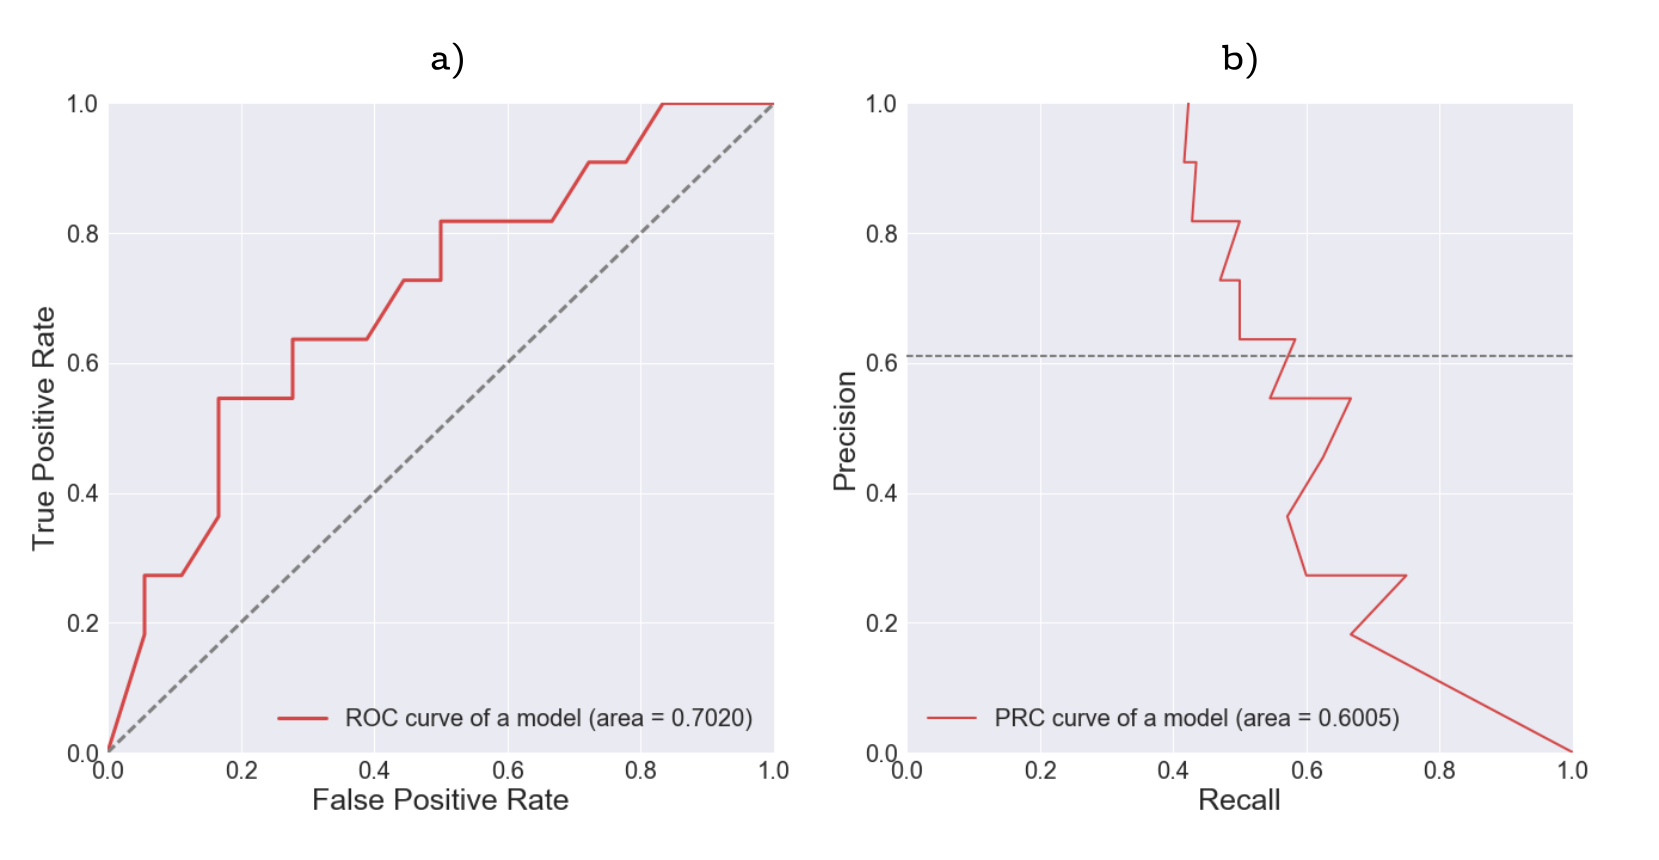
\includegraphics[scale=0.26]{roc_prc}
    \caption{Example of a) a \gls{roc} plot and b) a \gls{prc} plot.}\label{fig:roc_prc}
\end{figure}


For making decision, it is often important only a part of the \gls{roc} or \gls{prc} plot, for example the maximum of \gls{fp} or \gls{fn} is defined. There can be two curves A and B, which are crossing. It means that in the first part of the plot is, for example, the A curves above the B curves and in the second part, it is the opposite. If the first part of the plot is more important for prediction, then the selection of the model~A is better.


\section{Predictive methods}

There are a wide variety of predictive methods for classification which can be used and which accuracy can be compared. 

There are many simple but strong predictive methods based on statistical approaches and regression, such as a Naive Bayes, Linear regression, Logistic regression, Regression and classification trees and so on. These simple methods usually consist of one function or one principal which is optimised. 

On the other hand, there are a lot of advanced methods based on learning and optimising more complex functions. The structure of models can be huge and not easily understandable, but for complicated problems of the real word, it could be very powerful and efficient. 

These advanced methods are based on \gls{ann}s, ensembles of several models etc. In this thesis, I focused on few methods based on \gls{ann} and \gls{dt}, especially on Deep learning, Convolution and Recurrent Neural Network, Random Forest and Gradient Boosting Machines. 

\subsection{Neural networks methods}

The structure of \gls{nn}s is inspired by the biological neural network. There are units or artificial neurones, which are similar to biological neurones. The comparison of a biological neurone and an artificial neurone is in the figure~\ref{fig:ann}\cite{Johnson2017ann_intro}. These units are structured into layers. The layers are connected (often fully connected), and within a single layer share no connections, and form an acyclic graph (a network) with some inputs and outputs. The example of the whole network is in the figure~\ref{fig:ann_structure}.

\begin{figure}[ht]\centering
    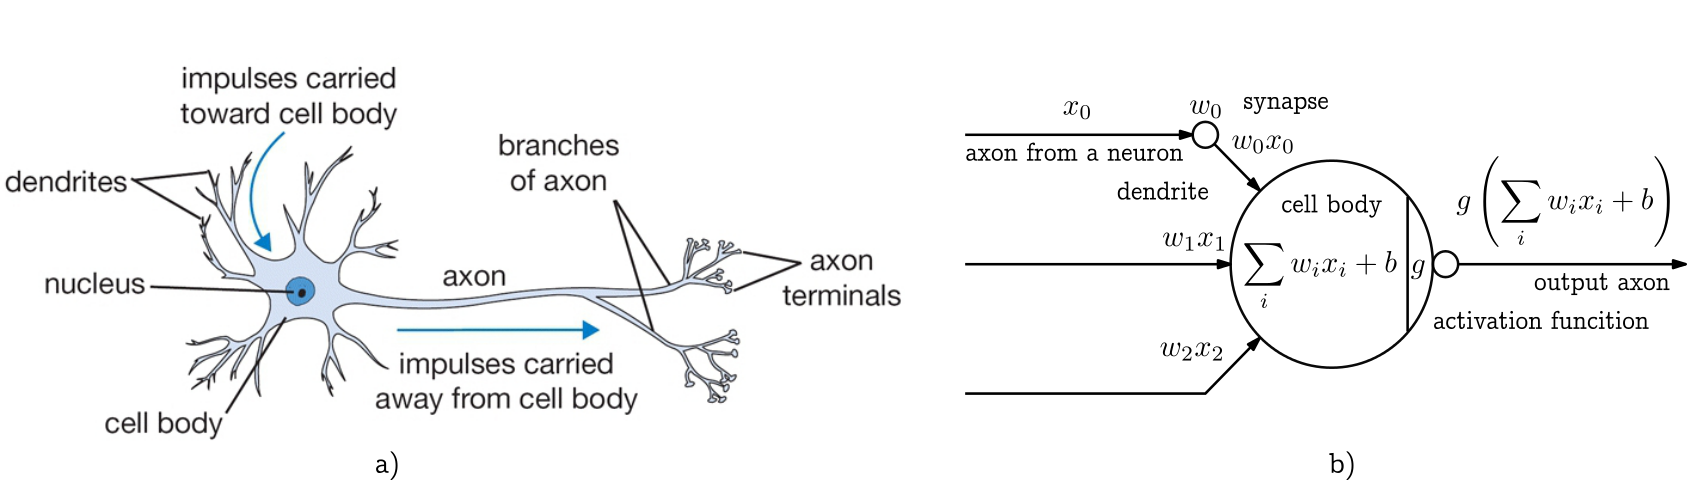
\includegraphics[scale=0.25]{ann2}
    \caption{Comparison of a) a biological neuron b) an artificial neuron (unit).}\label{fig:ann}
\end{figure}

\begin{figure}[ht]\centering
    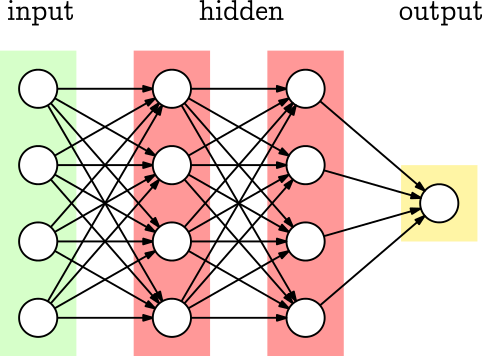
\includegraphics[scale=0.32]{nn}
    \caption{Example of a 2-hidden-layer \gls{ann}.}\label{fig:ann_structure}
\end{figure}

Each unit is a representation of a set of inputs, simple or complex function combining these input following the activation function, which output is also an output of the unit. There are three main types of \gls{ann} -- \gls{mlp} network also called \gls{dl} (based on basic idea, that through inputs the information is carried to the unit where information from inputs get weighted, summed and then the unit send another signal through the output to another unit), \gls{cnn} (contains convolution units which can be used for a processing more dimensional input such as images or signals) and \gls{rnn} (contains recurrent units, which can be used as a memory). However, a lot of modifications can be constructed because the all types of layers are easily connectable. 

\subsubsection{Deep learning}\label{sec:ann}

A single unit of \gls{mlp} network performs a dot product with the input ($x_i$ for example a single value from vector of observed data) and its weights ($w_i$), adds the bias vector ($b$) and applies the activation function ($g$) (adds non-linearity). The complete data transformation looks like $g(\sum_{i}{w_i x_i + b})$. 

The single neuron with defined loss function is a linear classifier.\cite{Johnson2017ann_intro} For example the $f(\sum_{i}{w_i x_i + b})$ can be interpreted as probability of one of the classes $\mathcal{P}(y_i|x_i;w)$. The probability of the other class would be $1-\mathcal{P}(y_i|x_i;w)$. Using this problem formulation and defined loss function (for example cross entropy loss) the problem would lead to a logistic regression.\cite{Johnson2017ann_intro}

The regular \gls{ann} consists of an input layer, a single hidden layer followed by an output layer. The neurones in each layer are fully connected with neurones from the following layer. Input layer is not count into number of layer, therefore the regular \gls{ann} is 2-layer \gls{nn}\cite{Johnson2017ann_intro} or one-hidden-layer \gls{mlp}\cite{theano_mlp}.  

Formally, a 2-layer \gls{nn} is a function $f: \Re^\mathcal{D} \rightarrow \Re^\mathcal{L}$, where $\mathcal{D}$ is the size of the input vector $x$ and $\mathcal{L}$ is size of the output vector $f(x)$. In matrix notation with bias vectors $b^{(1)}$, $b^{(2)}$, weight matrices $\mathbf{W}^{(1)}$ and  $\mathbf{W}^{(2)}$ and activation functions $G$ and $g$ \cite{theano_mlp}:

\begin{equation}
f(x) =  G(b^{(2)} + \mathbf{W}^{(2)}(g(b^{(1)} + \mathbf{W}^{(1)}x)))
\end{equation}

The activation function has to meet some requirements due to the learning process. It has to be non-constant, bounded, and monotonically-increasing continuous function. Using this function is guaranteed that the derivation exists and can be used during network learning. There are some base activations function for learning \gls{nn} -- Sigmoid, Tanh, \gls{relu} and Maxout\cite{Johnson2017ann_intro}.

The Sigmoid function takes a real-valued number and transforms it into the range between 0 and 1 -- in general, large negative numbers become 0 and large positive numbers become 1. The disadvantages of sigmoid function are that it saturates during learning and is not zero-centered. The Tanh function transforms a real-valued number to the range between -1 and 1. Like the sigmoid neurone, its activations saturate, but unlike the sigmoid neurone, its output is zero-centered. That is the reason why the Tanh is preferred to the Sigmoid. The \gls{relu} is linear and non-saturating and simply thresholded negative values at zero. The advantages of \gls{relu} are great acceleration the convergence of \gls{sgd} compared to the Sigmoid and Tanh and it is easy to compute. The disadvantage is that \gls{relu} can be deactivated during learning due to large gradient update. The last mentioned function is Maxout which is quite different because doubled \gls{relu} function (the \gls{relu} is the special type of Maxout function, where one input is always zero). This function benefits of \gls{relu} and is not deactivated during learning. However, the disadvantage is that it produce two times more parameters, which have to be optimised.\cite{Johnson2017ann_intro} The formal definitions of all mentioned function are in the table~\ref{tab:activations}.

{\renewcommand{\arraystretch}{1.7}%
\begin{table}[H]\centering
    \begin{small}
        \caption{Example the most common activation functions.}\label{tab:activations}
        \begin{tabular}{|l|c|}\hline
        Name of function & Formula \tabularnewline \hline \hline
        Sigmoid & $\sigma(x)=\frac{1}{1+e^{-1}}$ \tabularnewline \hline 
        Tanh & $tanh(x) =\frac{e^x - e^{-x}}{e^x+e^{-x}}$ \tabularnewline \hline 
        \gls{relu} & $ ReLu(x) = max(0,x)$ \tabularnewline \hline 
        Maxout & $ Maxout(x_1, x_2) = max(x_1, x_2)$ \tabularnewline \hline 
        \end{tabular}
    \end{small}
\end{table}}

The vector $h(x) = \Phi(x) = g(b^{(1)} + \mathbf{W}^{(1)} x)$ constitutes the hidden layer. $\mathbf{W}^{(1)} \in R^{D \times D_h}$ is the weight matrix connecting the input vector to the hidden layer. Each column $\mathbf{W}^{(1)}_{\cdot i}$ represents the weights from the input units to the $i$-th hidden unit. The output vector is then obtained as: $o(x) = G(b^{(2)} + W^{(2)} h(x))$.\cite{theano_mlp} 

To train the net, all parameters have to be optimised. The parameters to learn is the set $\theta = \{\mathbf{W}^{(2)},b^{(2)},\mathbf{W}^{(1)},b^{(1)}\}$. The gradients $\partial{\ell}/\partial{\theta}$ can be obtained using the backpropagation algorithm\cite{theano_mlp} -- the weights are updated according to the gradient. The gradient is propagated from output to input, computed using loss function $\ell(\mathbf{W, B|j})$ for all weights $\mathcal{W}$ and biases $\mathcal{B}$ in the net. For \gls{nn} classification is the loss function for example:

\begin{equation}
\ell(\mathbf{W, B|j}) = \sum_{\hat{y} \in O}{y^{(j)} log{(\hat{y}^{(j)})} + log{(1-\hat{y}^{(j)})}(1-y^{(j)})}
\end{equation}

\noindent where $\hat{y}$ is outputs from output layer and $y$ is true class.

Ordinary gradient descent is an optimising algorithm in which repeatedly making small steps downward on an error surface defined by a loss function of some parameters. \gls{sgd} works according to the same principles as ordinary gradient descent but proceeds more quickly by estimating the gradient from just a few examples at a time instead of the entire training set. In \gls{dl} Minibatch \gls{sgd} (MSGD) works identically to \gls{sgd}, except that there are used more than one training example to make each estimate of the gradient. This technique reduces variance in the estimate of the gradient, and often makes better use of the hierarchical memory organisation.\cite{theano_sgd} More about types of gradient descent method, which can be used during \gls{nn} learning, is in \cite{Qian1999sgd}.

\gls{nn}s could have only one hidden layer and be universal approximator \cite{Cybenko1989ann_aproximate} but they can also consist of many layers with many units. Even though the representational power is equal one hidden layer \gls{nn} and two hidden layer \gls{nn}, the deeper \gls{nn} can provide better prediction because the structure is more complex and can reflect the real data better, but it is just an empirical observation.\cite{Johnson2017ann_intro}

Regarding the problem of complexity of model mentioned in the section~\ref{sec:definitions}, there are several ways how to control the \gls{nn} to prevent overfitting. The most commons are L1 and L2 regularisation. L1  means that each weight $w$ is changed to $\lambda |w|$, where $\lambda$ is regularisation strength -- it leads the weight vectors to become sparse during optimisation, a sparse subset of the most important inputs is used and units become nearly invariant to the noisy inputs. L2 means for every weight $w$ in the network is changed to $\frac{1}{2}\lambda w^2$ where $\lambda$ is regularisation strength again -- it heavily penalise peak weights and prefers diffuse weight vectors, it allows the network to use all of its inputs a rather that some of its inputs a lot.\cite{Johnson2017ann_regularization} These two regularisations could be combined. The $\lambda$ hyperparameter is usually a small number, for example, $10^{-3}$. Finally, the result function to optimise is:

\begin{equation}
\ell'(\mathbf{W, B|j}) =  \ell(\mathbf{W, B|j}) + \lambda_1 L1(\mathbf{W, B|j}) + \lambda_2 L2(\mathbf{W, B|j})
\end{equation}

The Dropout is also very effective regularisation technique. While training, dropout is implemented by only keeping a neurone active with some probability $p$, or setting it to zero otherwise. Dropout can be interpreted as sampling a \gls{nn} within the full-connected \gls{nn}, and only updating the parameters of the sampled network based on the input data when the net is trained. During testing, there is no dropout applied -- the prediction is evaluated across the exponentially-sized ensemble of all sub-networks.\cite{Johnson2017ann_regularization} The hyperparameter $p$ is a value between 0 and 1, for example $0.2$. The example of the fully-connected network (a) and network with dropout (b) is in the figure~\ref{fig:dropout}.


\begin{figure}[ht]\centering
    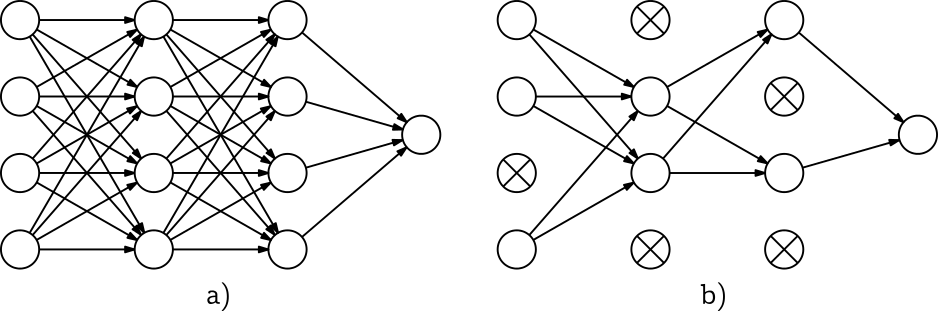
\includegraphics[scale=0.3]{dropout}
    \caption{Example of a) a fully-connected network and b) a network with dropout.}\label{fig:dropout}
\end{figure}

There are many other hyperparameters and settings (such as momentum, weight initialization, learning rate, a number of learning epochs, early stopping etc.), which can be set before training and can improve a prediction. Fortunately, there are many libraries or frameworks, which enable using \gls{nn} for prediction such as Caffe\cite{caffe}, Matlab\cite{matlab}, H2O\cite{h2o_DL_booklet} or Keras\cite{keras_soft}. It is good practice to read the documentation and learn how the \gls{nn} set or use the default setting. 

\subsubsection{Convolution Neural Network}\label{sec:cnn}

Convolutional Neural Networks (\gls{cnn} also called ConvNets) are similar to \gls{ann}.\cite{Johnson2017cnn} \gls{cnn} is consists of set of units (neurons) structured in layers which are connected and create a net. There are also weights and biases to optimise. Each neurone receives some inputs, performs a dot product and optionally follows it with an activation function. The whole network still expresses a single differentiable score function. Finally, there is a loss function on the last (fully-connected) layer, and all the tips for learning regular \gls{nn} still apply.

The main difference is a structure of the input. While the input of \gls{nn} is vector, the input of \gls{cnn} is \gls{3d} matrix (image with 3 colour channels, if the image is black and white the input has two dimensions only).\cite{Johnson2017cnn} There are several reasons,  why is this structure for learning better than a transformation of the \gls{3d} input into vector input and using standard \gls{nn}. 

Images have today usually size more than 200$\times$200$\times$3. When the image is transformed into vector, the vector size is 200$\times$200$\times$3 = 120\,000, it means 120\,000 weights in \gls{ann}. In this case, full connectivity is wasteful, and the huge number of parameters would quickly lead to overfitting. In an image, there is also important neighbourhood of pixels, which can be destroyed by the transformation into vector.\cite{Johnson2017cnn}

\gls{cnn} take advantage of the fact that the input consists of images (or signals), it has units arranged in three dimensions -- width, height and depth. The units in a layer are connected to a small region of the layer and every layer produce \gls{3d} output volume of units activations except the output layer which reduces the \gls{3d} input into a single vector (or single number). The example of a structure of \gls{cnn} is in the figure~\ref{fig:cnn}

\vspace*{0.5cm}

\begin{figure}[ht]\centering
    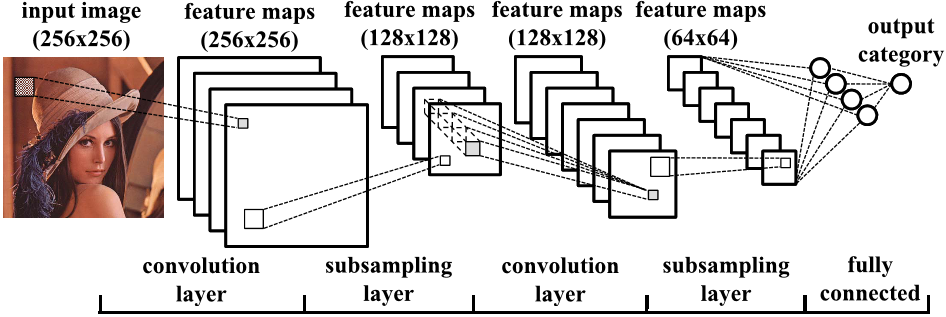
\includegraphics[scale=0.38]{lena}
    \caption{Example of a \gls{cnn} architecture.\cite{lena}}\label{fig:cnn}
\end{figure}

There are three main types of layers to build \gls{cnn} architecture -- convolutional, pooling and fully-connected layer. The weights of convolutional layer consist of a set of filters. Every filter is small (along width and height), but extends to the full depth of the input volume -- for example, a filter might have size 5x5x3 (for example 5 pixels width and height, and 3 pixels depth because of 3 colour channels). 

During the forward pass, the filters convolve each filter across the width and height of the input volume and compute dot products between the values of the filter and the input at any position. To reduce the number of parameters during learning, units in each depth slice (for example if the output volume is 10$\times$10$\times$5 there are 5 depth slices) will use the same parameters. So that means during backpropagation phase, every unit in the volume will compute the gradient for its weights, but these gradients will be added up across each depth slice and update a single set of weights per slice only. If the units use also the same weights during forwarding phase than the operation between filters and units is convolution.\cite{Johnson2017cnn} The \gls{2d} discrete convolution\cite{Ahn2014conv} is kind of image transformation and is defined as:

\begin{equation}
f[m, n] \ast g[m,n] = \sum_{j=1}^{J}\sum_{i=1}^{I} f[i,j]g[m-i, n-j]
\end{equation}

\noindent where in case of \gls{cnn} the $f$ is a slice, the $g$ is a filter, indexes $m$ and $n$ refer to the space of slice, the $I \times J$ is size of filter, where usually $I = J$. The example of the \gls{2d} convolution is in the figure~\ref{fig:convolution}

\begin{figure}[ht]\centering
    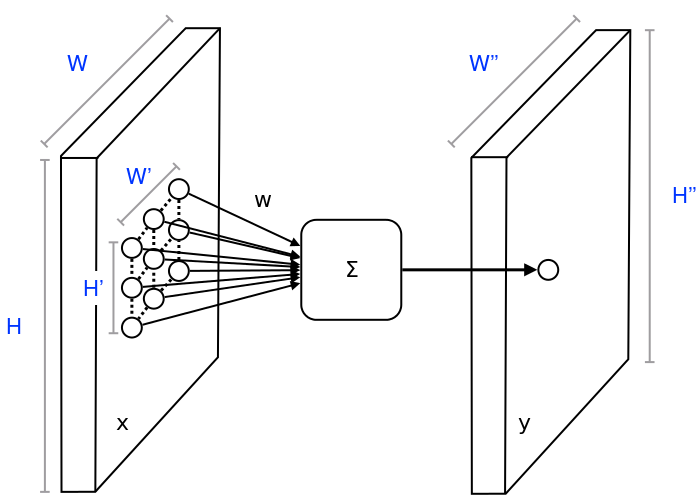
\includegraphics[scale=0.3]{conv}
    \caption{Example of \gls{2d} convolution.\cite{convolution}}\label{fig:convolution}
\end{figure}

As the filter slide over the width and height of the input volume, it produces a \gls{2d} activation map that gives the responses of that filter at every position. Each unit is connected to only a local region of the input volume. The spatial extent of this connectivity is a hyperparameter -- the receptive field of the unit (filter size). The number of units along the depth axis is equal to the depth of the input volume too. The connections are local along width and height, but full along the entire depth of the input volume.\cite{Johnson2017cnn}

The output size is controlled using three other hyperparameters -- fibre, stride and zero padding\cite{Johnson2017cnn}. Fibre is the depth of the output volume -- the number of filters in a layer. During learning, every filter learns a something different from the input, for example, different orientation of edges, colours, etc. The second parameter to set is stride which the filter slide over the image. If the stride is one, the filter slides per one pixel from left upper pixel to right lower pixel. If the stride is higher, it produces smaller output volumes. The last mentioned parameter is zero-padding, which to pad the input volume with zeros around the border. It allows controlling the size of the output volumes. The number of units in the layer can be computed as $(W-F+2P)/S+1$, where $W$ is the volume of input, $F$ is a number of filters, $P$ is a size of zero-padding, $S$ is a size of stride.

There are some constraints to choose a value of these hyperparameters. For example, if the setting is $P=(F-1)/2$ when the stride is $S=1$ it guarantees that input and output volume are the same. The stride setting sometimes can not fit input size so that some analysis of the size of preprocessing is necessary.

Another way how to reduce amount of parameters is using pooling layer between convolutional layers.\cite{Johnson2017cnn} The polling layer reduces the input volume using defined function over a defined subspace (usually maximum or average). The pooling operator has as filter defined size and stride and is applied independently on each depth slice. The size of polling is small (for example 2$\times$2) because of a small loss of information. During backpropagation, the gradient update is passed only on highest value in the forward pass.

For normalisation of values during training, there could be used normalisation layers, a simple function which changes all values in each depth slice of the input volume independently \cite{Johnson2017cnn}. The common function for normalisation is for example Tanh or \gls{relu}, which were defined in the table~\ref{tab:activations}.

The last type of layer which can be used in \gls{cnn} is a fully-connected layer, usually used as the output layer \cite{Johnson2017cnn}. All neurones are connected with the neurones from the previous layer, and it is the same layer as output layer in regular \gls{nn}. As defined in the section \ref{sec:ann}, the dropout can also be used.

The building of strong \gls{cnn}, which generalise well, depends on data. There are many hyperparameters and possibilities of the structure. In general, it is better to use more convolutional layers with more small filters, a small size of pooling operator and at the end fully-connected layer\cite{Johnson2017cnn}, but it is the only recommendation, it is not mathematically proven.

There are many of the \gls{cnn}s which can be widely reused. For example the simplest but strong structure of \gls{cnn} is LeNet-1 introduced by Yan LeCunn et. all in 1989 \cite{Lecun1989cnn}, which was used to recognise handwriten zip code digits. Simply, the LeNet structure is $Input \rightarrow Convolution \rightarrow Tanh \rightarrow Pooling \rightarrow Convolution \rightarrow Tanh \rightarrow Pooling \rightarrow Fully\,connected \rightarrow Tanh \rightarrow Fully\,connected$ and is demonstrated in the figure~\ref{fig:lenet}.

\begin{figure}[ht]\centering
    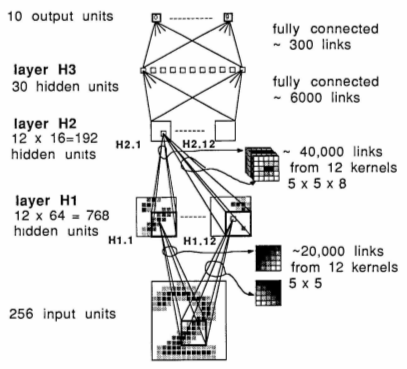
\includegraphics[scale=0.7]{lenet1}
    \caption{The LeNet-1 architecture. \cite[548]{Lecun1989cnn}}\label{fig:lenet}
\end{figure}

\subsubsection{Recurrent Neural Network}

The last \gls{nn} which I mentioned is \gls{rnn}. As I introduce in section~\ref{sec:ann} the \gls{ann} is an acyclic graph, however in case of \gls{rnn}, it is not true. The \gls{rnn} consists of the special layer which has a loop. The loop allows information to be passed from one step of the network to the next respect the time (or sequence of inputs). Simply the \gls{rnn} is able to learn some context from input data. In some cases, it is very useful to learn information sequentially for example in natural language processing or time series analysis.  

If the hidden layer with the loop is unrolled, the structure of the \gls{rnn} is more visible (and is also important for training). There is not loop, but a deep network with one hidden layer per time step and shared weights across time steps. There is input layer which takes the first element of the current sequence (time step), then the second and so on. Then, there are recurrent units which take own input, the output from their predecessor and own state and do some operation. Then the result is sent to output and their successor.\cite{Lipton2015rnn} The example of the structure of \gls{rnn} is in the figure~\ref{fig:rnn}

\begin{figure}[ht]\centering
    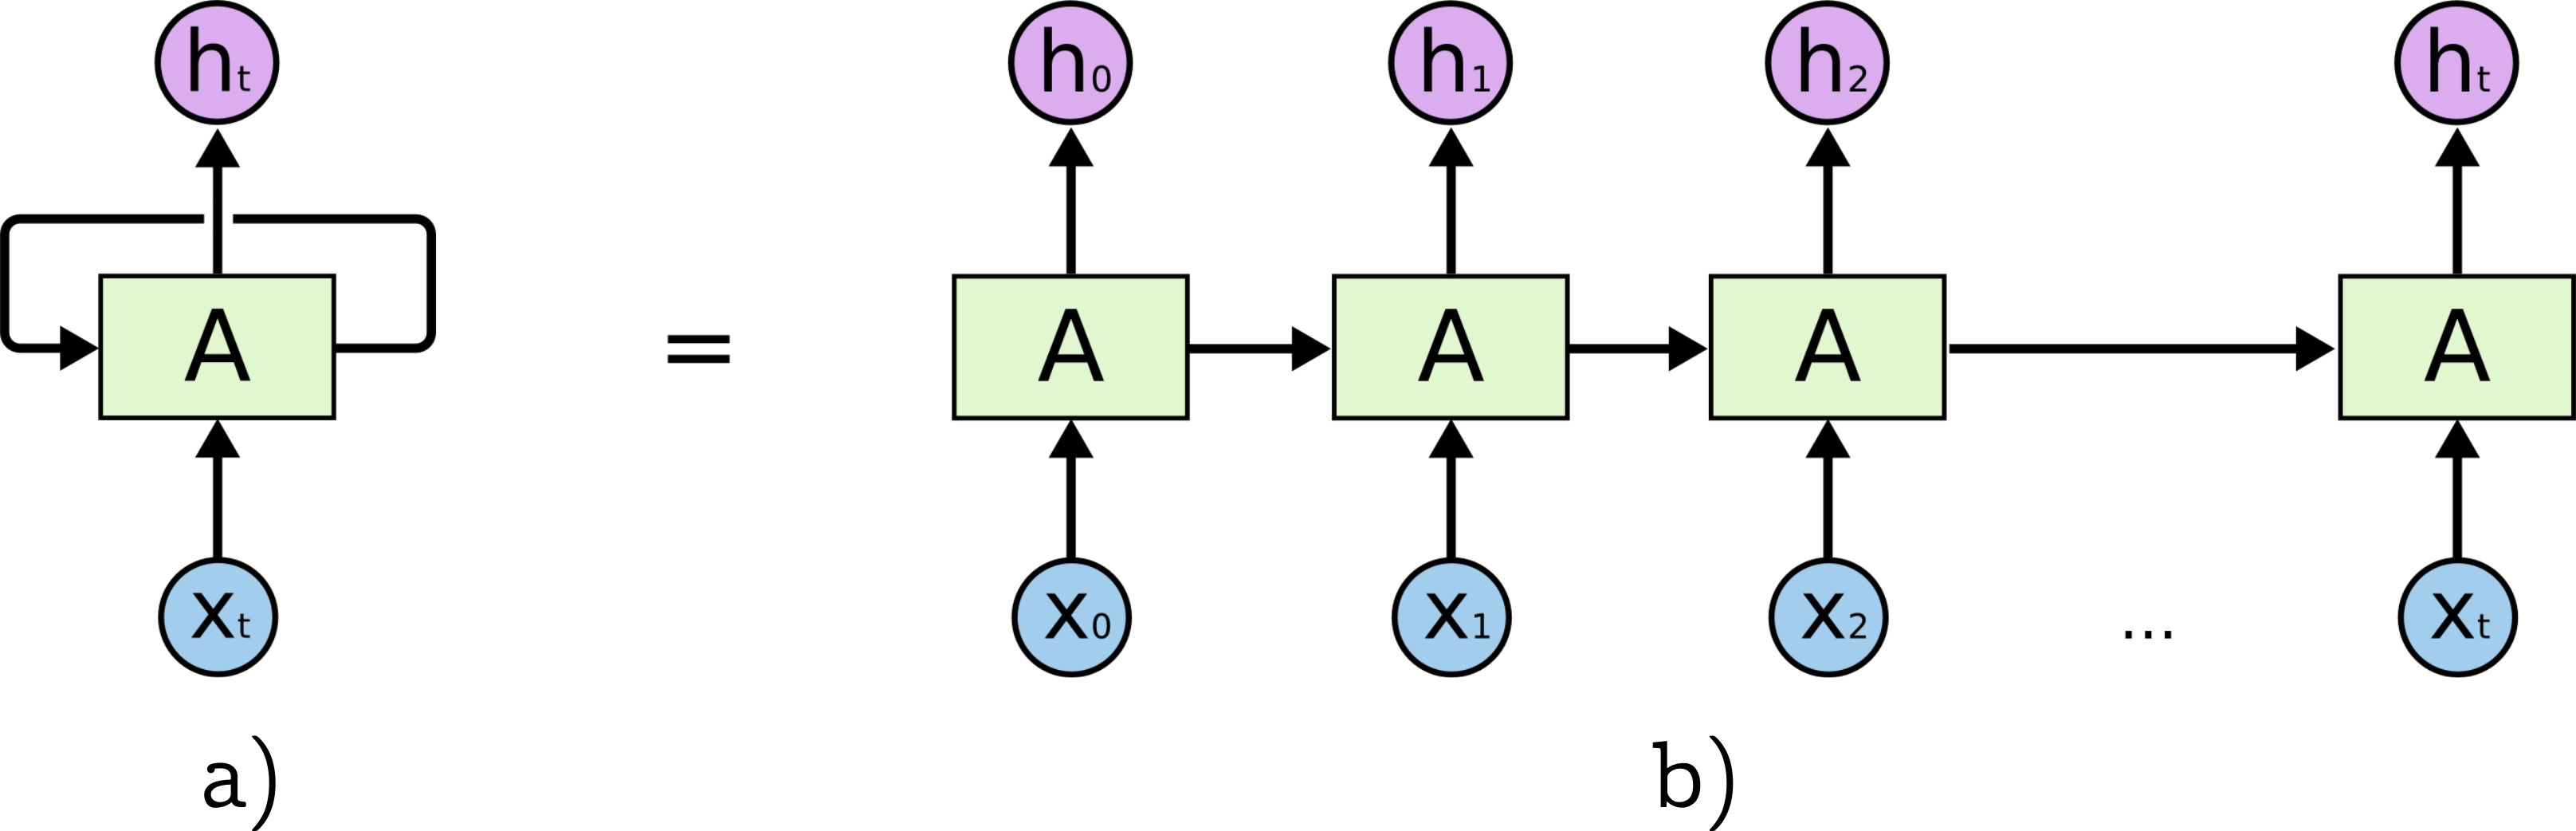
\includegraphics[scale=0.1]{lstm_unrolled}
    \caption{Structure of a \gls{rnn} a) with loop b) unrolled.\cite{lstm_images}}\label{fig:rnn}
\end{figure}

The task of standard recurrent unit is very simple. There are one hidden state $s_t$ which is calculated from the previous hidden state $s_{t-1}$ multiplied by matrix of state weights $V$ and the input $x_t$ in time $t$ which multiplied by matrix of input weights $U$ using an activation function $f$ (the types of activation function are the same as for \gls{ann}, for example Tanh or \gls{relu}). At the end in the output layer for example softmax is applied. The weight are shared across all units during one sequence pass. The schema of this unit is in the figure~\ref{fig:sru}. The mathematical formula of the simple \gls{rnn} is:

\begin{equation}
\begin{multlined}
s^{(t)} = f(\mathbf{U} x_{(t)} + \mathbf{V} s^{(t-1)} + b_h) \\ 
\hat{y} = softmax(\mathbf{O} h^{(t)} + b_y)\\
\end{multlined}
\end{equation}

\begin{figure}[ht]\centering
    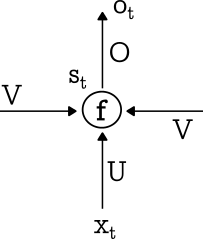
\includegraphics[scale=0.6]{sru}
    \caption{The schema of standard recurrent unit.}\label{fig:sru}
\end{figure}

In general, \gls{rnn}s combine the input vector with their state vector with a fixed function to produce a new state vector. This can in be interpreted as a program with certain inputs and some internal variables. Similar to universal approximation theorem mentioned in section~\ref{sec:ann}, there will be proven, that RNNs are Turing-Complete in the sense that they can to simulate arbitrary programs (with proper weights) \cite{Siegelmann1991turing}. However, out of math theory, it is not realisable yet. 

The unfolded network can be trained using backpropagation similar to \gls{ann} but across many time steps. This algorithm, called \gls{bptt} it is more complicated than standard backpropagation algorithm using partial derivation and its explanation is out of scope this thesis. More about \gls{bptt} can be learnt from the article\cite{Werbos1990bptt}, where it was introduced by Werbos in 1990. 

In the context of the backpropagation in standard, \gls{rnn} one problem are known -- vanishing and exploding gradients occur when backpropagating errors across many time steps\cite[13--14]{Lipton2015rnn}. It means that \gls{rnn} is able to remember the short context of input information because weights are not fixed against to vanish or explode. Due to this problem, new types of the hidden unit with memory were developed.

The most common \gls{rnn} with memory  is \gls{lstm}\cite[17]{Lipton2015rnn}. The structure is the same compared to standard \gls{rnn} except the units in hidden layer were replaced by memory cells (more complex structure with several units inside). Each memory cell contains a node with a self-connected recurrent edge of fixed weight one. It ensures that the gradient can pass across many time steps without vanishing or exploding. The schema of the \gls{lstm} cell is in the figure~\ref{fig:lstm} 

\begin{figure}[ht]\centering
    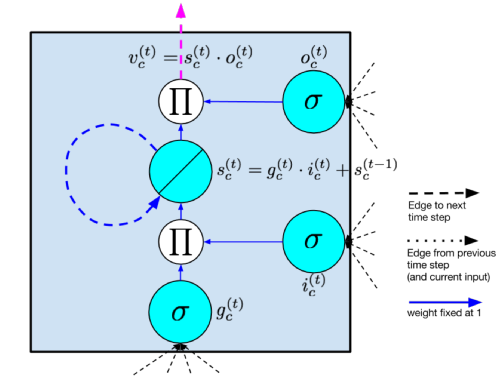
\includegraphics[scale=0.35]{lstm}
    \caption{The schema of \gls{lstm} cell.\cite[17]{Lipton2015rnn}}\label{fig:lstm}
\end{figure}


In a simplified way, in the \gls{lstm} cell, there are several units -- input node $g$, input gate $i$, internal state $s$, forget $f$ gate and finally output gate $o$. The input and output gates control the input and output into the memory cells. The forget gate learns to reset the inner state of the memory cell when its context is too old. In mathematical formula\cite[20]{Lipton2015rnn} the complete computation of one time step in \gls{lstm} cell is:

\begin{equation}
\begin{multlined}
g^{(t)} = tanh(\mathbf{W}^{gx}x^{(t)} + \mathbf{W}^{gh} h^{(t-1)} + b_g)\\
i^{(t)} = \sigma(\mathbf{W}^{ix}x^{(t)} + \mathbf{W}^{ih} h^{(t-1)} + b_i)\\
f^{(t)} = \sigma(\mathbf{W}^{fx}x^{(t)} + \mathbf{W}^{fh} h^{(t-1)} + b_f)\\
o^{(t)} = \sigma(\mathbf{W}^{ox}x^{(t)} + \mathbf{W}^{oh} h^{(t-1)} + b_o)\\
s^{(t)} = g^{(t)} \odot i^{(t)} + s^{(t-1)} \odot f^{(t)}\\
h^{(t)} = tanh(s^{(t)}) o^{(t)}\\
\end{multlined}
\end{equation}

\noindent where $\sigma$ is sigmoidal function (for example \gls{relu}), $\mathcal{W}$ are weights of the all units across the cell, $b$ are bias of the all units across the cell, $h^{t}$ is the vector of values from hidden layer and $h^{t-1}$ is the values output by each memory cell in the hidden layer at the previous time.  

There are many other useful modifications of \gls{rnn}. For example Bidirectional \gls{rnn}, Stack \gls{rnn}, \gls{rnn}-EM etc.\cite{Lipton2015rnn} 

\subsection{Decision Trees methods}\label{sec:trees}

Decision making is the task which everyone comes into contact with it every day. There are often a large number of different factors which have to be taken into account, and there are a lot of possibilities how to evaluate which impact the different alternatives will have. Behind this, the decision trees were developed not only for computer science and machine learning but also for economics, social studies etc.

The decision tree is in general acyclic graph which has hierarchical tree structure -- it means there is a root node, which has children nodes (subtree) connected branches with parent and at the end, there are leaf nodes, which have no children. The root node is at the first decision level, at the next levels there are decisions influenced by the decision making on the first level and so on.

In predictive analysis are decision trees used for classification and regression too. It is a large family of simple but strong algorithms for many classification and regression tasks based on binary trees. The tree building is based on hierarchical splitting the training data into two subsets according to contained information. In the decision nodes, conditions are derived, and the final predictions are situated in the leaf nodes. Using the conditions in the decision nodes the prediction is decided based on the terminal leaf node, where the new data end during passing through a tree. The example of a \gls{dt} is in the figure~\ref{fig:dt}.

\begin{figure}[ht]\centering
    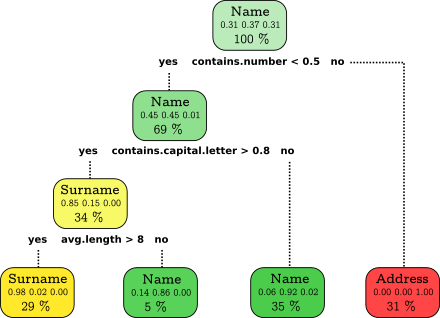
\includegraphics[scale=0.3]{tree}
    \caption{Example of a simple decision tree.}\label{fig:dt}
\end{figure}

The most important part of three building is a criterion for splitting the data toward one feature (attribute)\cite{Quinlan1986dt}. There are several criteria which can be used -- entropy, information gain, Gini index etc. There are the most common splitting functions in the table~\ref{tab:criterion}. According to the splitting criterion, the classification problem is optimised -- the goal is to split data across the most informative features and to build as small tree as possible.

{\renewcommand{\arraystretch}{1.7}%
\begin{table}[H]\centering
    \begin{scriptsize}
        \caption{Example the most common splitting functions for binary classification (where $S =(S_1, S_2, \cdots S_n)$ is subset of training data across the values $v$ of one feature (attribute) $A$, $p(1|x)$ is probability that a element $x$ has class '1', $S_v$ is subset of system $(S,A)$ which contains only value $v$ from $A$).}\label{tab:criterion}
        \begin{tabular}{|l|c|}\hline
        Function name & Formula  \tabularnewline \hline
        Entropy & $ H(X) = - p(0|x) \log{p(0|x)} - p(1|x) \log{p(1|x)} $  \tabularnewline
        Entropy of system $(S, A)$ & $ E(S, A) = \sum_{v \in Values(A)}{\frac{|S_v|}{|S|} H(S_v)}$  \tabularnewline
        Information gain of system $(S,A)$ & $I(S, A) = H(S) - E(S , A)$\tabularnewline\hline
        Gini index & $Gini(X) = 1 - p(0|x)^2 - p(1|x)^2 $ \tabularnewline
        Gini inpurity of system $(S,A)$ & $I_G(S,A) = \sum_{v \in Values(A)}{\frac{|S_v|}{|S|} Gini(S_v)} $\tabularnewline\hline
        \end{tabular}
    \end{scriptsize}
\end{table}}

The learning algorithm starts with whole training dataset. The dataset is recursively split by values of the feature using splitting criterion until the subset of data is not able to split. For example, if in the leaves, there are data only with one class, or the classification error is less than defined threshold, or the maximum depth of the tree is reached.\cite{Quinlan1986dt}  The minimal number of data in the parent or leave nodes, maximum depth, the criterion for splitting are hyperparameters of \gls{dt}.

There are some other techniques to regularise learning, such as pruning of branches -- reducing some branches which are modelling for example noise instead of data distribution or generalise of function for splitting -- instead of hyperplane orthogonal to axes to use quadratic or different hyperplane.\cite{Deng2011dt}

The advantages of decision trees are simple implementation and training, the model could be strong with a small amount of data, and the result is not the only prediction, but the \gls{dt} also detect the feature importance.  The disadvantage are that single \gls{dt}s can be overfitted with more complex problem and with categorical features which are biased in favour of those features with more levels.\cite{Deng2011dt}

To build a more powerful model with complex data, and avoid instability of \gls{dt} methods (in bias and variance of error), the algorithm based on ensembling were developed. The ensemble is set of techniques how to combine many models together and get a better prediction. There are some techniques based on the training data, for example cross-validation (mentioned briefly in the section~\ref{sec:definitions}), bagging and boosting.\cite[5--6]{Dietterich2000ensamble} 

Bagging is algorithm where from the original training dataset several new training sets are generated by sampling uniformly and with replacement from the original dataset. Then one model is trained on each new training set, and the final class is decided based on the majority vote. Boosting also uses a sampling of original training data but builds new models sequentially according to the error on the previously fitted model. The most widely used algorithms based on \gls{dt} and ensembling are \gls{rf} and \gls{gbm}.

\subsubsection{Random Forests}\label{sec:rf}

Random forests are based on bagging algorithm and are combination of \gls{dt} predictors. Each \gls{dt} is fitted on the part of data sampled randomly and independently but with the same distribution. For tree building can be used random feature selection or other types of randomness. All single predictors from a forest and the result classification is decided by the voting of individual trees. The accuracy of a random forest depends on the strength of the individual tree classifiers and a measure of the dependence between them.\cite[1--3]{Breiman2001rf} 

The algorithm to build \gls{rf} model is simple. First for each \gls{dt}, choose at random and with replacement, $n$ observations
among $n$ from the training dataset. Then build each \gls{dt} independently from another, without pruning. For split select at random a subset variables for each created node. The example of \gls{rf} classifier is in the figure~\ref{fig:rf}

\begin{figure}[ht]\centering
    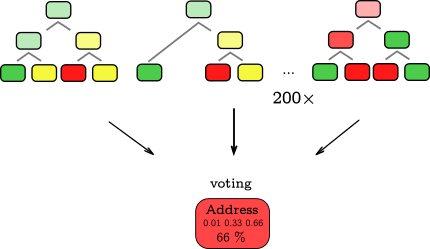
\includegraphics[scale=0.3]{rf}
    \caption{Example of a \gls{rf} classifier.}\label{fig:rf}
\end{figure}

Breiman proved, that increasing number of trees in \gls{rf} algorithm reduces bias and does not overfit\cite{Breiman2001rf}. He also proved that \gls{rf} give results competitive with boosting and adaptive bagging. Another advantage of \gls{rf} is that the algorithm is easy to parallelise -- thousands of trees can be processed at the same time. Finally, if the data are changed a little the forest is more stable to predict correctly than a single \gls{dt}

The hyperparameters important in \gls{rf} are number max depth of trees and number of trees in an ensemble, but many others parameters which affect tree building and are the same for standard \gls{dt} which can improve prediction. 

\subsubsection{Gradient Boosting Machines}

Contrary to \gls{rf} Gradient Boosting Machines are based on boosting algorithm. The predictors can be \gls{dt} but also different standard predictors can be used. The main idea is to build a lot of weak models so that the models are not built independently and do not split the training dataset. The new model is fitted using information about the error from the previous model. The resulting predictor is the combination of all models. Function estimation is viewed as a numerical optimisation in function space, rather than parameter space. \cite{Friedman2000gbm}

The algorithm to build \gls{gbm} model for binary classification is iterative and is more complicated than \gls{rf} algorithm. The algorithm ends, if the maximum number of iterations $M$ is reached or some other condition is met.  First, it choose the loss function $\ell(y, F)$ for boosting optimisation. For classification is the loss function called negative binomial log-likelihood:

\begin{equation}
\ell(y, F) = \log{(1+e^{-2yF(x)})}, y \in {0,1}
\end{equation}

\noindent Initialise $F_0(x) = {arg\,min}_{\gamma} \sum_{i}F(y_i,\gamma) $. Repeat $M$ times following: Compute the pseudo-response $\hat{y}$ as:

\begin{equation}
\hat{y}_i = - \left[\frac{\partial\ell(y_i,F(x_i))}{\partial F(x_i)}\right]_{F(x) = F_{m-1}(x)}
\end{equation}

\noindent Then fit \gls{dt} $h_m(x)$ with the train data with targets $\hat{y}$. The $h_m(x)$ split the input into $J_m$ disjoint regions $R_{1m}, \cdots R_{J_mm}$. For each region find $\gamma_{jm}$ which is computed by solving optimisation problem:

\begin{equation}
\gamma_{jm} = {arg\,min}_{\gamma} \sum_{x_i \in R_{jm}}{\ell(y_i, F_{m-1}(x_i) + \gamma)}
\end{equation}

Than define indicator function $I(x \in R_{jm})$ which returns 1 if given $x$ is in the given region $R_{jm}$, 0 otherwise. The final model $m$th iteration is:

\begin{equation}
F_m(x) = F_{m-1}(x) + \sum_{j=1}^{J_m}{\gamma_{jm} I(x \in R_{jm})}
\end{equation}

The final model is the last $F_M(x)$ which was built. If there is not any restriction, the constructed trees tend to be large especially during the early iterations. To avoid this phenomenon, maximum depth of all trees are defined. The recommendation is to choose smaller trees (weak predictor) rather than large ones. For example a model consists of lot of trees with $J = 2$ (stumps) can be very strong.\cite[362]{Hastie2001statisticallearning}

There are other regularisation techniques.\cite[361--365]{Hastie2001statisticallearning} A number of iteration $M$ is one of them. Shrinkage regularisation it to select some hyperparameter $v \in (0,1)$ to scale tree built in each iteration. Smaller $v$ means larger training risk for fixed $M$. Both $M$ and $v$ control prediction risk on training data, however, these parameters are dependent. Smaller value of the $v$ lead to larger value of the $M$. The recommended strategy is to select $v$ very small and then choose $M$ by early stopping.\cite[364]{Hastie2001statisticallearning} To improve the performance of a noisy predictor, the subsampling technique, which is similar to bagging, can be used. At each iteration, the data are sampled into sample without replacement, and the tree is built only using this sample of data.

\begin{figure}[ht]\centering

    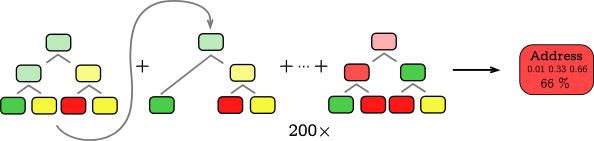
\includegraphics[scale=0.3]{gbm}
    \caption{Example of a \gls{gbm} classifier.}\label{fig:gbm}
\end{figure}
\vspace*{0.5cm}

Compared to \gls{rf}, the \gls{gbm} tend to overfit, for example, if the size of trees is too large or number or iteration is too high. However, with correct hyperparameter setting could be \gls{gbm} also the strong predictor. The example of a \gls{gbm} predictor building is in the figure~\ref{fig:gbm}.

\subsection{Hyperparameter optimisation}

The performance of each model which was mentioned is affected by some hyperparameters. For example, the number of units in the hidden layer, number of layers influence predictive power of \gls{nn}, the size of trees or number of the tree in an ensemble is important for \gls{rf}. If some regularisation techniques are used, the setting of coefficients is crucial. Also characteristic of data is fundamental for correct parameter setting, so default setting could not bring success. Therefore searching correct parameters are necessary.

With growing computing power and increasing memory space available in computers, the manual hyperparameter search is a waste of time. Therefore some methods of hyperparameter search were developed - for example, grid search, random search or Bayesian optimisation.

The easiest methods how to search defined space of hyperparameters is using grid search. The models are trained with cartesian product of given sets of hyperparameters and the result of defined metrics is computed. Then the best model is chosen for prediction. But this approach is computationally exacting and could run for a long time.

Random search (also called direct-search) are optimisation methods, which do not require the gradient of the problem, so that not continuous or differentiable functions can be optimised.\cite{Bergstra2012rs} For given function (for example loss function) and defined space of parameters, random parameters are chosen, and functional value of the function is computed. Until a termination criterion is met (for example optimal value is reached or a number of iterations performed) the new position in hyperparameter space is randomly select with some defined radius. If the value of a new position is better than the new step is initialized from this position. Finally, the best model is chosen for prediction. This simple technique can found the same optimal model but faster. The other advantage is that the parameter space could be better searched because using a grid some hyperparameters could be omitted. The difference between grid search and random search is showed in the figure~\ref{fig:search}.

\begin{figure}[ht]\centering
    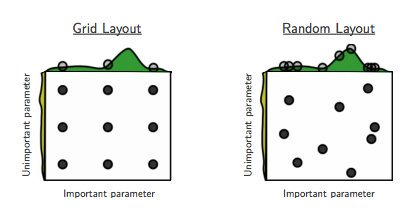
\includegraphics[scale=0.6]{grid_search}
    \caption{Comparison of the grid search and the random search.\cite[284]{Bergstra2012rs}}\label{fig:search}
\end{figure}

Finally, there are several modifications of random search or other different techniques. For example, hyperparameter search using Bayesian optimisation -- fitting of a probabilistic model based on evaluation of functions and their parameters to predict which parameter configuration is the best.\cite{Snoek2012bopt} This method can find the minimum of difficult non-convex functions with a few evaluations, at the cost of performing more computation to determine the next point to try. It could be useful if the evaluation of model loss function is very expensive.

%%%%%%%%%%%%%%%%%%%%%%%%%%%%%%%%%%%%%%%%%%%%%%%%%%%%%%% CHAPTER %%%%%%%%%%%%%%%%%%%%%%%%%%%%%%%%%%%%%%%%%%%%%%%%%%%%%%%

\chapter{Analysis based on real-world crime data}\label{analysis}

Crime prediction is not an easy task; criminality is a phenomenon which occurs seemingly random. However, in data are often hidden information, which human are not able to process. To find out more about the hidden information, the data have to be analysed using sophisticated methods. This is exactly what this chapter is about -- analysing the real data using supervised learning to try to find out a hidden pattern of occurring crime in the Czech Republic. 

In the first section, the definition of objectives and methodology are described. The second part of the process is one of the most important parts, and it is about crime data understanding and preprocessing. The following section is about experiment setting, and the next is about predictive models building. Using methods based on \gls{nn} and \gls{dt}, the best model was found for predicting crime. Finally, the results are evaluated, compared and summarised. 

All steps of the analysis are described in details to be easily repeated in police practice. One part of this thesis are scripts, which was developed for analysis of real data and can be reused for further research. 

\section{Methodology and Business understanding}

The whole analysis is based on the \gls{crisp} process, which was described in the theory part of this thesis. This thesis is focused only on analysis. Thus the business understanding, data understanding, data preparation, modelling and evaluation parts are described. The deployment is out of scope this thesis. 

For analysis and experiments, I obtained unexplored crime data from the \gls{pcr}. The data contain a full history of crimes which occurred in the Czech Republic and was registered by \gls{pcr}.

The main reasons why analyse these data are: to determine the quality of data, to gain insight into the issue of criminality in the Czech Republic, to detect risk areas and to develop preventive actions. From the point of view predictive analysis, the hidden crime patterns can be found and used for crime prevention. However, is it possible to make a short-term prediction using these data and tools of predictive analysis, especially with supervised learning? How accurate will these predictions be? 

The Hot-spot analysis, Risk-terrain analysis Spatio-temporal analysis and other techniques are useful especially for medium-term or long-term predictions. Near-repeat analysis is useful only for the special type of crime and is able to identify pattern only with additional personal data in small areas. The data mining techniques give plenty of possibilities how data can be analysed. The primary objectives of the analysis in this thesis are:

\begin{enumerate}
    \item Preprocess non-personal crime data from the database of the \gls{pcr} and define important information therein.
    \item Find out how accurate short-term predictions can be obtained using these data and supervised algorithms.
    \item Find out which type of information is the most important in predictive modelling using supervised algorithms. 
    \item Try to improve the accuracy of predictive models.
    \item Summarise which models with which type of information are the best. 
\end{enumerate}

Many tools, programming languages and libraries were used -- all of them are open source. I used \gls{sql} and R language to get and join important data for analysis. Using Python, I did the rest of the analysis from data preprocessing to build predictive models and evaluate results. Except for analysis, the output is are also scripts, which were used to process and analyse data. 

\section{Crime data understanding and preparation}\label{sec:preprocessing}

If data are wrongly interpreted, or any fault is done during processing and data transformation, analysis and result can be incorrect. With real data, plenty of operations has to be done, much more than with preprocessed datasets. Every data transformations which were done I describe in this section.

\subsection{Data source}

The \gls{pcr} provided the data in the PostgreSQL database dump format. The database consists of 17 tables. There is a main table which contains crime data history and many other tables which are connected to the main table by foreign keys and contain additional information about crimes such as names of crime types, names of regions, exact coordinates for different rasters, information about clarifies or distances from some point of interest, etc.

\begin{figure}[ht]\centering
    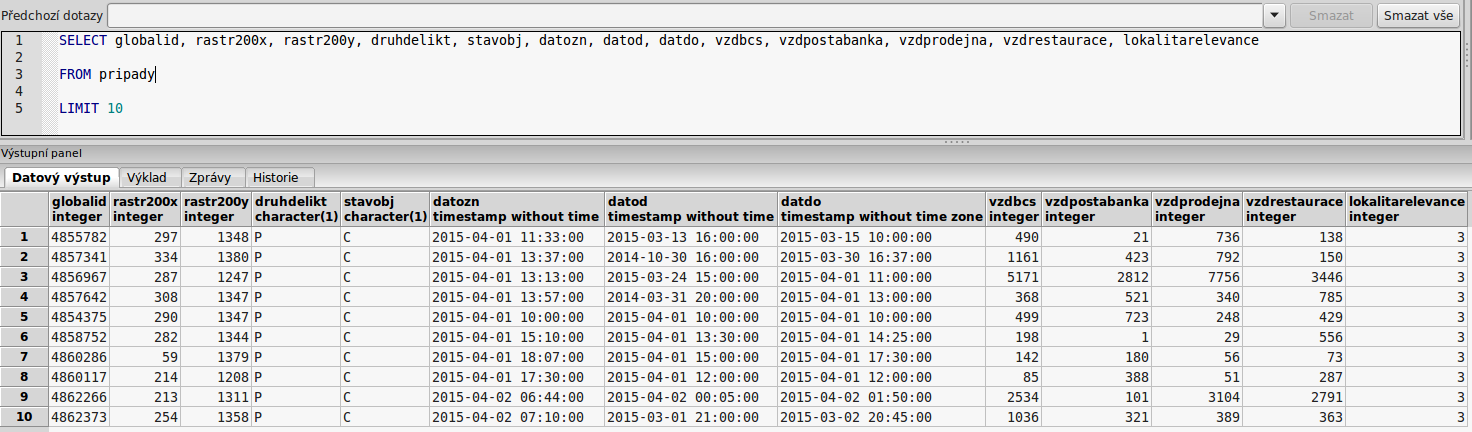
\includegraphics[scale=0.25]{database}
    \caption{Example of data viewed using pgAdmin tool.}\label{fig:database}
\end{figure}

\subsection{Data joining, selecting and cleaning}

Data in \gls{sql} database are not suitable for data analysis with tools such as R or Python. Better manipulation is with data joined into one or more datasets and exported them from the database into a text file. The main table contains string codes of crime type and the foreign key to the main table and tables contain coordinates which determinate a position of squares on the map of the Czech Republic were exported. 

The first step was to filter specific types of crime. It requires joining of main table and table with types because each crime in the database has several types of labels (for example four and more). For whole analysis, I choose only types of crime which frequently occurs in general, for example, bicycle theft or burglary of an apartment. 

% vloupání do bytu D.01, Krádeže motorových vozidel - dvoustopých E.01, Krádeže součástek a věcí (nebo PHM) z motorových vozidel včetně vloupání E.05

The second step was selection only Prague city area to reduce data quantity. All raster information tables with the result from the previous step were joined and all data between Prague's border plus some extra squares around were selected. The extra squares were useful for padding data in the next data processing. You can see selected area using QGIS in the figure~\ref{fig:prague_selected}. Some of the squares are on the border between Prague and another region. I had to correct these squares to have the only one region flag. I assigned Prague flag all crime records connected with these squares.

\begin{figure}[ht]\centering
    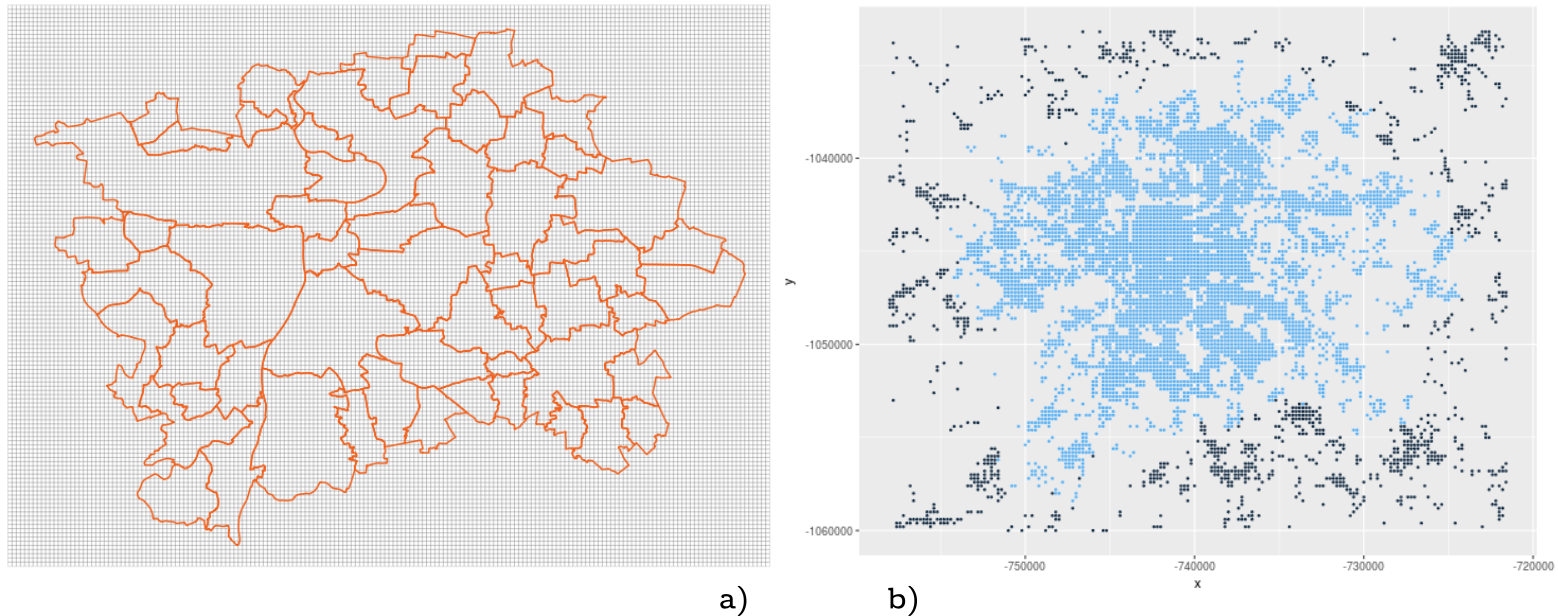
\includegraphics[scale=0.29]{praha_sel}
    \caption{Example of selected area for analysis -- a) selected grid 200~m $\times$ 200~m b) rectangles where at least one crime occurred and assigned flag of Prague.}\label{fig:prague_selected}
\end{figure}

The next step was focused on date columns. Crime occurring date (from, to) and crime recorded date was separated into new columns (minute, hour, day, weekday, week, month, year). From the hour and month information, the category was extracted (hour category -- morning, forenoon, noon, afternoon, night and month category -- spring, summer, autumn, winter). Then the occurring date interval was inspected whenever is not too long. Intervals longer than 5 days or shorter than -1 day (this type of error was found in the dataset, for example, because of time shift and system incompatibility) was removed from the dataset. The only one date had to be selected, and therefore I selected start date of the interval for analysis.

The \gls{pcr} has started the collection of data with coordinates since July 2013. Data before this date is poor because the \gls{pcr} generated coordinates from recorded address. They can not regenerate a big amount of data, and I got data without these records. The histogram of crime count per year is in the figure~\ref{fig:crime_histogram} (One record from 1900 was removed so that the histogram is readable). For analysis, the data from 1 January 2013 were selected.

\begin{figure}\centering
    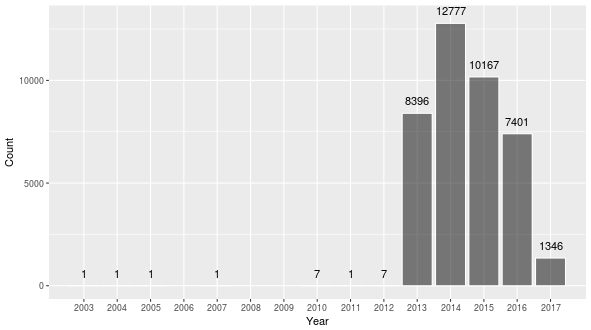
\includegraphics[scale=0.4]{crime_histogram}
    \caption{Histogram of crime count per year selected crime type.}\label{fig:crime_histogram}
\end{figure}

After cleaning phase, I transformed some categorical features into one-hot encoding to improve predictions. For example, the clarification of the crime which consists of 7 classes (A = clarify directly, B = clarify additionally, C = unclarified, etc.). After one-hot encoding, the dataset contained new seven columns with only 0-1 values.

Finally, I grouped data by square ID and date. New column \texttt{crimecount} was created. If there were more than one crime in one square, the data were grouped. The new row contains the sum of information from all these rows. You can see the example of this process in the figure~\ref{fig:grouped_data}.

\begin{figure}[ht]\centering
    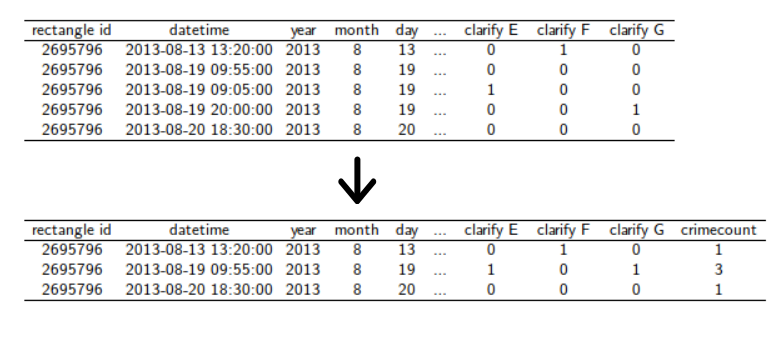
\includegraphics[scale=0.4]{grouped_data}
    \caption{Example of grouped data.}\label{fig:grouped_data}
\end{figure}

\subsection{Basic analysis}

After all these preparation of data, the result datasets contained 38 columns. I prepared four different types of crimes, and all these datasets have three version because of three types of raster (size of the square edge 100, 200 or 500 metres). Datasets have from 6000 to 60000 rows approximately. For the following analysis, the only dataset was chosen due to time and memory complexity of the problem. I chose the 200~m $\times$ 200~m grid, which contains 5939 individual squares. The following graphs and results are based only on these data.  

To understand data, I made some basic statistics using selected dataset. In the table~\ref{tab:summary_ba}, you can see the short summary of the data. In the figure~\ref{fig:histograms_ba}, there are histograms for some features individually (without normalisation).

\begin{table}[H]\centering
    \caption{Selected dataset summary.}\label{tab:summary_ba}
    \begin{tabular}{|l|l|}\hline
        rows & 37~907 \tabularnewline \hline
        columns & 38 \tabularnewline \hline
        min date & 2013-01-02 \tabularnewline \hline
        max date & 2017-03-07 \tabularnewline \hline
        total number of days & 1~525 \tabularnewline \hline
        total number of unique squares & 5~939 \tabularnewline \hline
        %& \tabularnewline \hline
    \end{tabular}
\end{table}

\begin{figure}[ht]\centering
    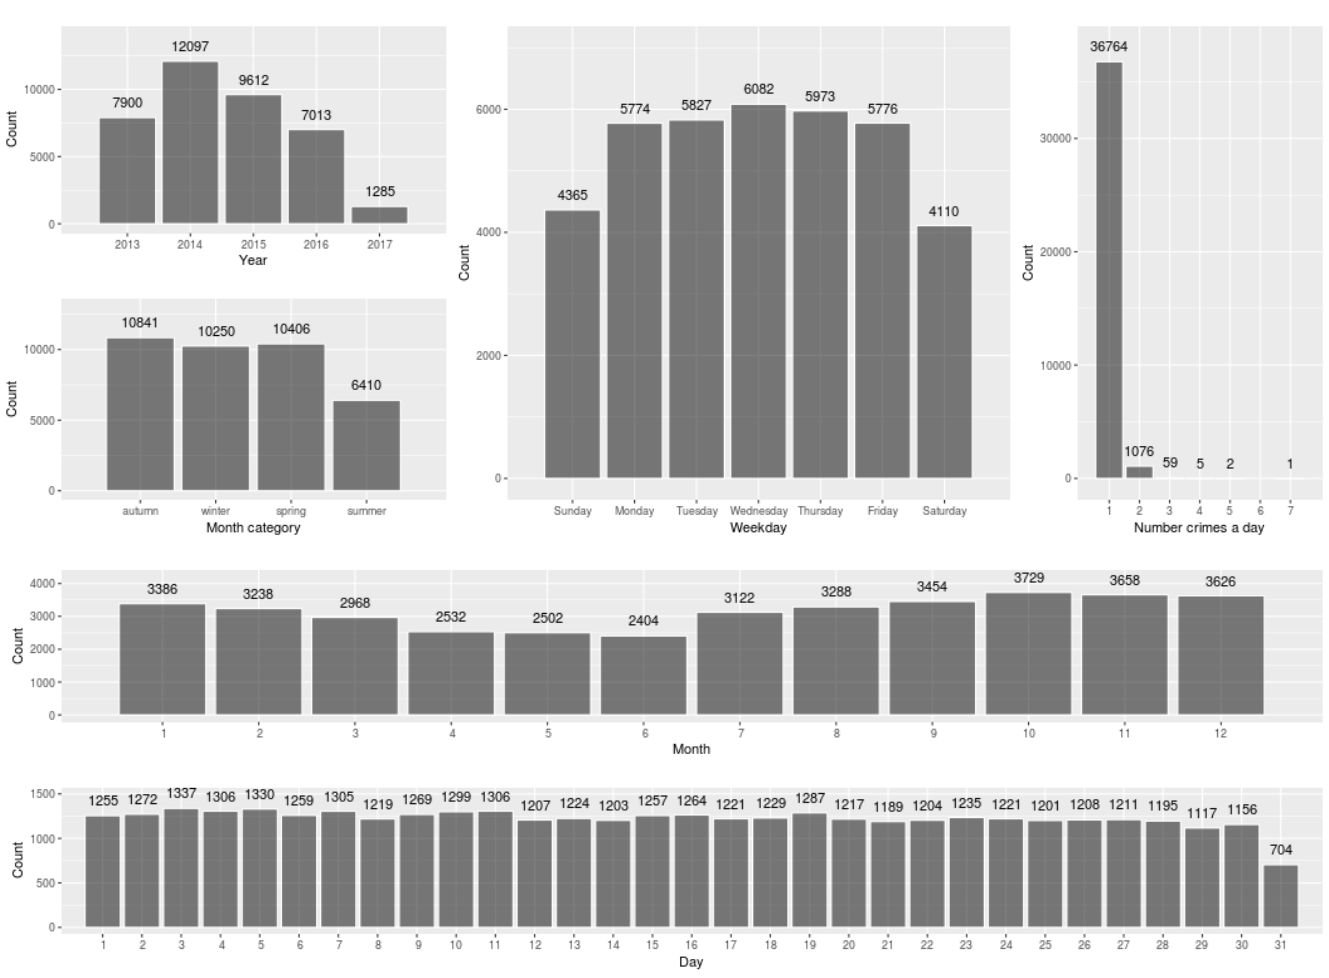
\includegraphics[scale=0.34]{histograms_ba}
    \caption{Histograms of selected and preprocessed data.}\label{fig:histograms_ba}
\end{figure}

\subsection{Feature extraction}

During data cleaning, some new features were extracted, for example, date columns from separation, columns from one-hot encoding, results from data grouping. However, a lot of other possibilities to extract new information from data exist. First I extracted new features using time and space information from data, and then I used \gls{pca} to try to get new useful columns.

\subsubsection{Create new features from data}

The dataset contains a lot of information about time and space where crime often occurred. The main idea of my analysis was, how much is possible to predict feature crime from near past and close space distance. However, the dataset contains only crime history, where a crime occurred, and for prediction is useful to know days, where a crime did not happen too. The next step was to generate the days with zero crime count. 

To inspect the past, I generated time series of crime count per day for every square (in the range defined previously), where at least one crime occurred. After basic analysis, I decided to change date interval. I analysed data from 7 July 2013 to 8 March 2017 and created time series and other datasets in this interval.

Using window method the time series was cut into smaller intervals -- 21 days long only. For example, the first record is connected with 7 July 2013; its new time series start from 16 June 2013 to 6 July 2013. This approach generated 21 new features. Using this dataset I can analyse, how the 21 days long past crime history affected crime next day. 

I used time series dataset also for neighbour arrays generating. The neighbour array consists of squares close to a certain distance. I selected distance five and therefore result array dimensions are 11 $\times$ 11 ($5 + 1 + 5 = 11$). That is why the extra squares around selected area were useful. This approach generated 120 new features. 

All data in the dataset are connected with a date and crime count. But it is not possible to get all these information to predict whenever the crime occurs on the same day. I decided to analyse yesterday's situation only, and therefore I had to shift all data except date and crime count one day to the feature. The result is that I have a date and associated crime count as a feature, and I have the situation from the previous day crime history.  

\subsubsection{Extract features using \gls{pca}}

The \gls{pca} method is very useful tool for feature extraction. This method is used mainly for dimension reduction, but it could be helpful in prediction problem too. It assigns a new vector (or single number depends on the settings of \gls{pca} method) to all data records. These new features can improve prediction.

I decided to apply this method to all features in the dataset and select the five most important components. So that, this method generated five new features.


\subsection{Feature selection}\label{sec:feature_selection}

The last part of data preprocessing is feature selection. The main goal of feature selection is also to reduce data dimension space, but the information from removed features is lost. There are several methods to select features based on regression, statistical tests or decision tree algorithms. 

At the end of preprocessing method which generated new feature, the final dataset contained 173 features. The list of all features and a short explanation are is in the table~\ref{tab:fs_summary}.

{\renewcommand{\arraystretch}{2}%
\begin{table}[H]\centering
    \begin{scriptsize}
    \caption{Features summary.}\label{tab:fs_summary}
        \begin{tabularx}{\textwidth}{p{2cm}|X|c}
    Feature name & Description & Count \tabularnewline\hline\hline
    Rectangle\_ID & identifier of observed square & 1\tabularnewline\hline
    Latitude, Latitude\_ID, Longitude, Longtitude\_ID & coordinate definition of observed square & 4 \tabularnewline\hline
    Loc\_relevancy & number which indicate if assigned location is relevant  & 1\tabularnewline\hline
    Day, Weekday, Week, Month, Month\_cat, Year & date definition of observed day & 6 \tabularnewline\hline
    Di\_rest, Di\_postbank, Di\_shop, Di\_gas & distance of the nearest restaurant, post office or bank, shop, gas station & 4 \tabularnewline\hline
    Hour\_cat\_n & number of crimes which occurred the day before observed day, division into hour categories, where n = 1 is hour interval from  0-5h, n = 2 is hour interval from  5-9, n = 3 is hour interval from  9-12, n = 4 is hour interval from 12-18 and n = 5 is hour interval from  18-24 & 5 \tabularnewline\hline
    Clarify\_X & number of crimes which occurred the day before observed day with X clarify class & 6 \tabularnewline\hline
    Neigh\_n & n-th position in 11 $\times$ 11 sized neighbour array, where n=60 is central square & 121 \tabularnewline\hline
    Day\_n & crime count in n-th day from 21 long time series where n=21 is a day before observed day & 21\tabularnewline\hline
    PCA\_n & n-th component from \gls{pca} (index is from 0 to 4) & 5\tabularnewline\hline
        \end{tabularx}
    \end{scriptsize}
\end{table}}


I combined a few feature selection methods together (Correlation (CORR), Lasso (LASSO), \gls{lr}, \gls{rf}, \gls{rfe} and \gls{rr}). I normalised columns with crime count to 0-1 interval before. The result of feature ranking (top 42 the most important feature) is in the table~\ref{tab:fs_result}. The results of the individual method are normalised by a number of all features to the 0-1 interval. The final ranking (RANK) is computed from an average of results from all methods (AVG). 

\begin{table}\centering
    \begin{scriptsize}
    \caption{Selected features summary.}\label{tab:fs_result}
    \begin{tabular}{|c|l|c|c|c|c|c|c|c|}\hline
Rank & Feature & CORR & LASSO & LR & RF & RFE & RR & AVG\tabularnewline\hline\hline
1 & PCA\_0 & 1.00 & 1.00 & 0.00 & 0.23 & 0.89 & 0.00 & 0.52\tabularnewline\hline 
2 & Dist\_rest & 0.86 & 0.75 & 0.00 & 0.12 & 0.92 & 0.00 & 0.44\tabularnewline\hline 
3 & Day\_21 & 0.47 & 0.00 & 1.00 & 0.00 & 1.00 & 0.05 & 0.42\tabularnewline\hline 
4 & Neigh\_60 & 0.47 & 0.00 & 0.85 & 0.00 & 1.00 & 0.05 & 0.40\tabularnewline\hline 
5 & Day\_15 & 0.37 & 0.00 & 0.00 & 0.03 & 0.80 & 1.00 & 0.37\tabularnewline\hline 
6 & Day\_7 & 0.36 & 0.00 & 0.00 & 0.03 & 0.79 & 1.00 & 0.36\tabularnewline\hline 
7 & Day\_20 & 0.33 & 0.00 & 0.00 & 0.04 & 0.72 & 0.92 & 0.33\tabularnewline\hline 
7 & Day\_10 & 0.31 & 0.00 & 0.00 & 0.03 & 0.75 & 0.88 & 0.33\tabularnewline\hline 
8 & Day\_8 & 0.31 & 0.00 & 0.00 & 0.03 & 0.69 & 0.87 & 0.32\tabularnewline\hline 
9 & PCA\_4 & 0.01 & 0.00 & 0.00 & 1.00 & 0.86 & 0.00 & 0.31\tabularnewline\hline 
10 & Dist\_postbank & 0.80 & 0.00 & 0.00 & 0.12 & 0.91 & 0.00 & 0.30\tabularnewline\hline 
10 & Day\_19 & 0.29 & 0.00 & 0.00 & 0.03 & 0.65 & 0.84 & 0.30\tabularnewline\hline 
10 & Day\_1 & 0.29 & 0.00 & 0.00 & 0.03 & 0.64 & 0.84 & 0.30\tabularnewline\hline 
11 & Day\_17 & 0.28 & 0.00 & 0.00 & 0.03 & 0.64 & 0.81 & 0.29\tabularnewline\hline 
11 & Day\_2 & 0.28 & 0.00 & 0.00 & 0.03 & 0.63 & 0.81 & 0.29\tabularnewline\hline 
11 & Day\_4 & 0.27 & 0.00 & 0.00 & 0.03 & 0.63 & 0.80 & 0.29\tabularnewline\hline 
12 & Day\_9 & 0.26 & 0.00 & 0.00 & 0.03 & 0.61 & 0.76 & 0.28\tabularnewline\hline 
12 & Day\_5 & 0.24 & 0.00 & 0.00 & 0.03 & 0.66 & 0.72 & 0.28\tabularnewline\hline 
13 & Day\_16 & 0.26 & 0.00 & 0.00 & 0.03 & 0.62 & 0.74 & 0.27\tabularnewline\hline 
13 & Day\_6 & 0.25 & 0.00 & 0.00 & 0.03 & 0.62 & 0.74 & 0.27\tabularnewline\hline 
13 & Day\_18 & 0.23 & 0.00 & 0.00 & 0.03 & 0.66 & 0.69 & 0.27\tabularnewline\hline 
13 & Day\_3 & 0.22 & 0.00 & 0.00 & 0.03 & 0.67 & 0.67 & 0.27\tabularnewline\hline 
14 & Day\_13 & 0.25 & 0.00 & 0.00 & 0.03 & 0.54 & 0.73 & 0.26\tabularnewline\hline 
14 & Clarify\_C & 0.48 & 0.00 & 0.02 & 0.01 & 0.96 & 0.09 & 0.26\tabularnewline\hline 
15 & Hour\_cat\_5 & 0.21 & 0.00 & 0.25 & 0.01 & 1.00 & 0.06 & 0.25\tabularnewline\hline 
15 & Hour\_cat\_4 & 0.17 & 0.00 & 0.25 & 0.01 & 1.00 & 0.09 & 0.25\tabularnewline\hline 
15 & Clarify\_F & 0.01 & 0.00 & 0.02 & 0.00 & 0.95 & 0.51 & 0.25\tabularnewline\hline 
15 & Year & 0.51 & 0.00 & 0.00 & 0.12 & 0.84 & 0.02 & 0.25\tabularnewline\hline 
15 & Day & 0.00 & 0.00 & 0.00 & 0.62 & 0.85 & 0.00 & 0.25\tabularnewline\hline 
16 & Dist\_shop & 0.44 & 0.00 & 0.00 & 0.11 & 0.89 & 0.00 & 0.24\tabularnewline\hline 
16 & Hour\_cat\_3 & 0.06 & 0.00 & 0.25 & 0.00 & 1.00 & 0.12 & 0.24\tabularnewline\hline 
17 & Hour\_cat\_2 & 0.03 & 0.00 & 0.25 & 0.00 & 0.99 & 0.08 & 0.23\tabularnewline\hline 
17 & Latitude & 0.27 & 0.06 & 0.00 & 0.08 & 0.93 & 0.00 & 0.23\tabularnewline\hline 
18 & PCA\_1 & 0.05 & 0.25 & 0.00 & 0.15 & 0.88 & 0.00 & 0.22\tabularnewline\hline 
18 & PCA\_3 & 0.12 & 0.00 & 0.00 & 0.28 & 0.91 & 0.00 & 0.22\tabularnewline\hline 
18 & Day\_14 & 0.29 & 0.00 & 0.00 & 0.04 & 0.13 & 0.84 & 0.22\tabularnewline\hline 
18 & Latitude\_ID & 0.27 & 0.00 & 0.00 & 0.08 & 0.93 & 0.00 & 0.22\tabularnewline\hline 
19 & Neigh\_71 & 0.07 & 0.00 & 0.00 & 0.03 & 0.83 & 0.36 & 0.21\tabularnewline\hline 
19 & Hour\_cat\_1 & 0.02 & 0.00 & 0.25 & 0.00 & 0.99 & 0.03 & 0.21\tabularnewline\hline 
19 & Neigh\_49 & 0.07 & 0.00 & 0.00 & 0.03 & 0.82 & 0.34 & 0.21\tabularnewline\hline 
19 & Weekday & 0.03 & 0.00 & 0.00 & 0.37 & 0.83 & 0.00 & 0.21\tabularnewline\hline 
19 & Neigh\_59 & 0.06 & 0.00 & 0.00 & 0.03 & 0.82 & 0.33 & 0.21\tabularnewline\hline 
    \end{tabular}
    \end{scriptsize}
\end{table}

In the table~\ref{tab:fs_result}, following interesting discoveries can be observed. First, on the top of the most exciting features, were ranked components from \gls{pca} in average, but it is not surprising because the components were computed from all features and used an orthogonal transformation of data, so the first components has o lot of information. 

Secondly, the information about the distance of some points of interest (restaurants, post offices, etc.) were also selected as important in many methods. From neighbours, the most significant are 60, 71, 49 and 59, which are very close neighbours. Other neighbours squares are at the end of ranking. From time series is the most important that the day before the observed day (feature name Day\_21) and other day are also on the top. The Day\_21 and Neigh\_60 has same values (except \gls{lr}), because it has the same information. In the model, where was combined place and time information, one of these features was dropped out.

I used these 42 features in models, where I combined time and place information together. In the section~\ref{sec:tm_neigh_information} is the comparison of models which were built with all features and with selected features only.

\subsection{Result datasets}\label{sec:result_datasets}

Due to memory and time complexity, I had to select a smaller area than before. New area contains 50 $\times$ 50 squares. However, for data preparation, I used 5 square at each side, and therefore the result used area contains 40 $\times$ 40 squares only. The summary of this new dataset is in the table~\ref{tab:fdataset_summary} and a view of selected area is in the figure~\ref{fig:subprague}.

\begin{table}[H]\centering
\begin{small}
    \caption{Selected dataset summary.}\label{tab:fdataset_summary}
    \begin{tabular}{|l|l|}\hline
        rows &  1~740~618\tabularnewline \hline
        columns & 172 \tabularnewline \hline
        min date & 2013-06-17 \tabularnewline \hline
        max date & 2017-03-08 \tabularnewline \hline
        total number of days & 1~341 \tabularnewline \hline
        total number of unique squares & 1~298 \tabularnewline \hline
        %& \tabularnewline \hline
    \end{tabular}
\end{small}
\end{table}

The final preparation of data is to divide them into three subsets -- training, validation and test data. I decided to sort them by date and split data with regard to time and place to maintain a trend information. The training data contain records from 7 July 2013 to 30 January 2016 (938 days), validation data contain records from 31 January 2016 to 25 October (268 days), and finally, the test data contain record from 26 October to 8 March 2017 (135 days). The proportion of the each class in particular subset is shown in the figure~\ref{fig:data_split}. 

\begin{figure}[ht]\centering
    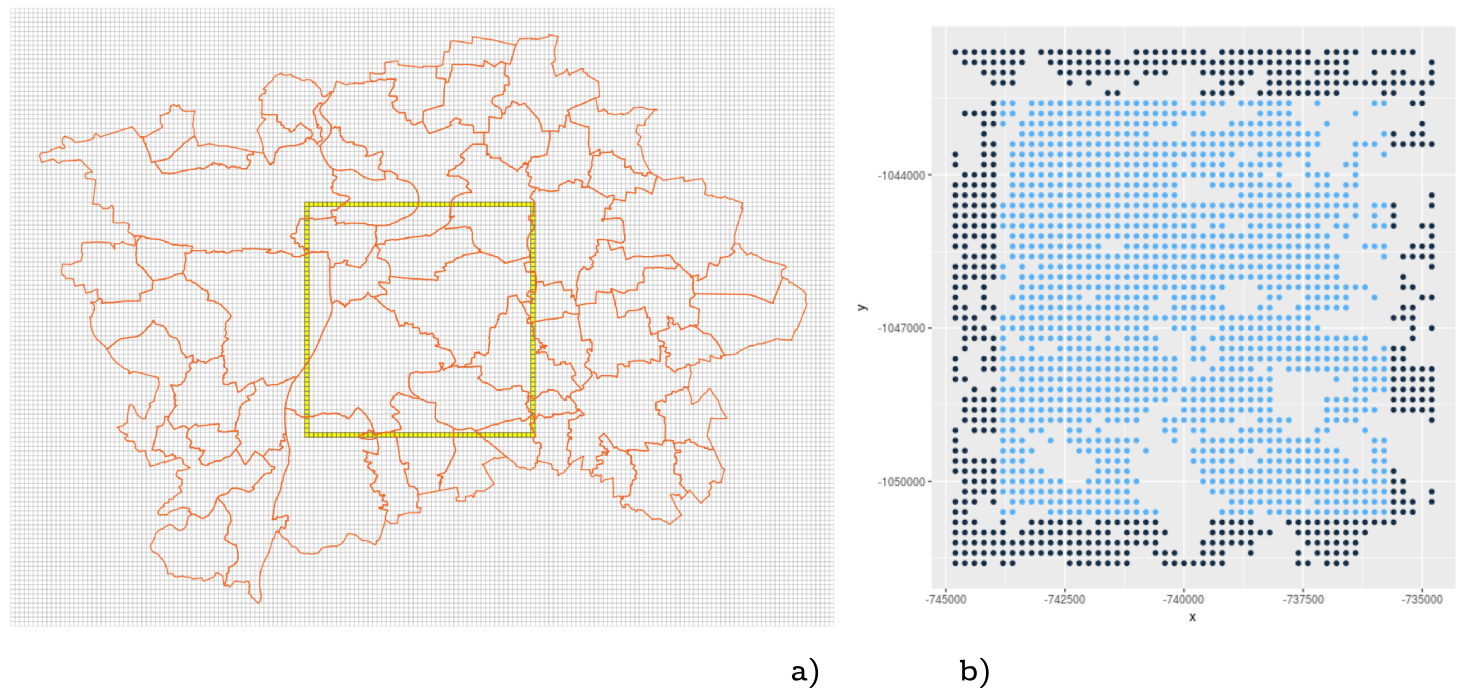
\includegraphics[scale=0.29]{subprague_sel}\label{fig:subprague}
    \caption{Example of new selected subarea for analysis -- a) position of selected subarea in grid 50 $times$ 50 rectangles, b) rectangles where at least one crime occurred and flag for preprocessing.}
\end{figure}

\begin{figure}[ht]\centering
    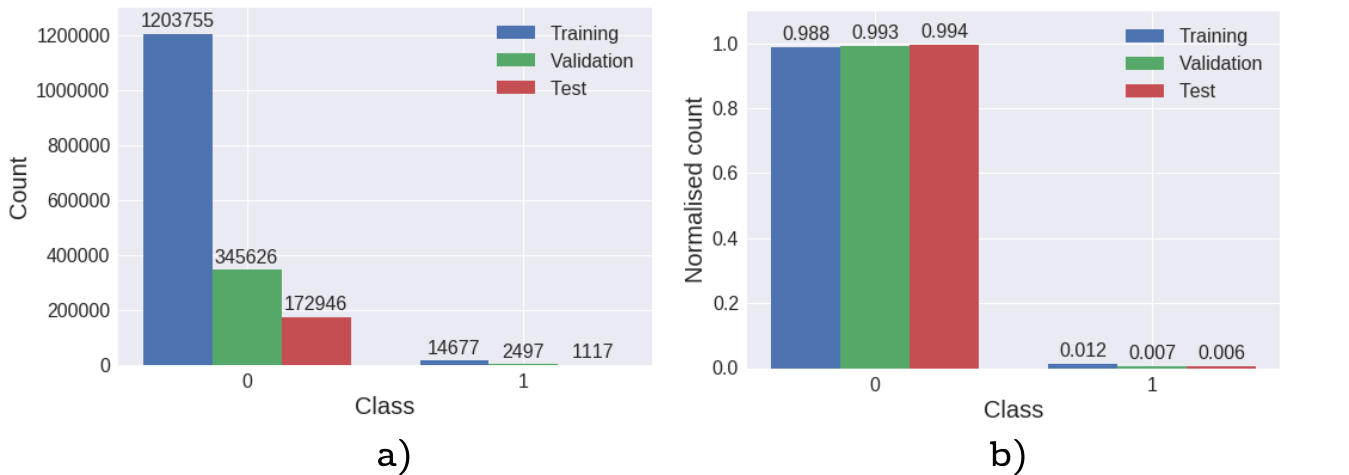
\includegraphics[scale=0.27]{data_split_b}\label{fig:data_split}
    \caption{Example of separated data and proportion of the classes -- a) count of each class in particular set, b) normalised count of each class in particular set.}
\end{figure}

To summarise, three types of data were prepared -- based on time information, place information and the combination of both. The types of data are represented in the figure~\ref{fig:data_types}. Then I had to select smaller area, and finally, I split the data into a format suitable for predictive analysis. 

\begin{figure}[ht]\centering
    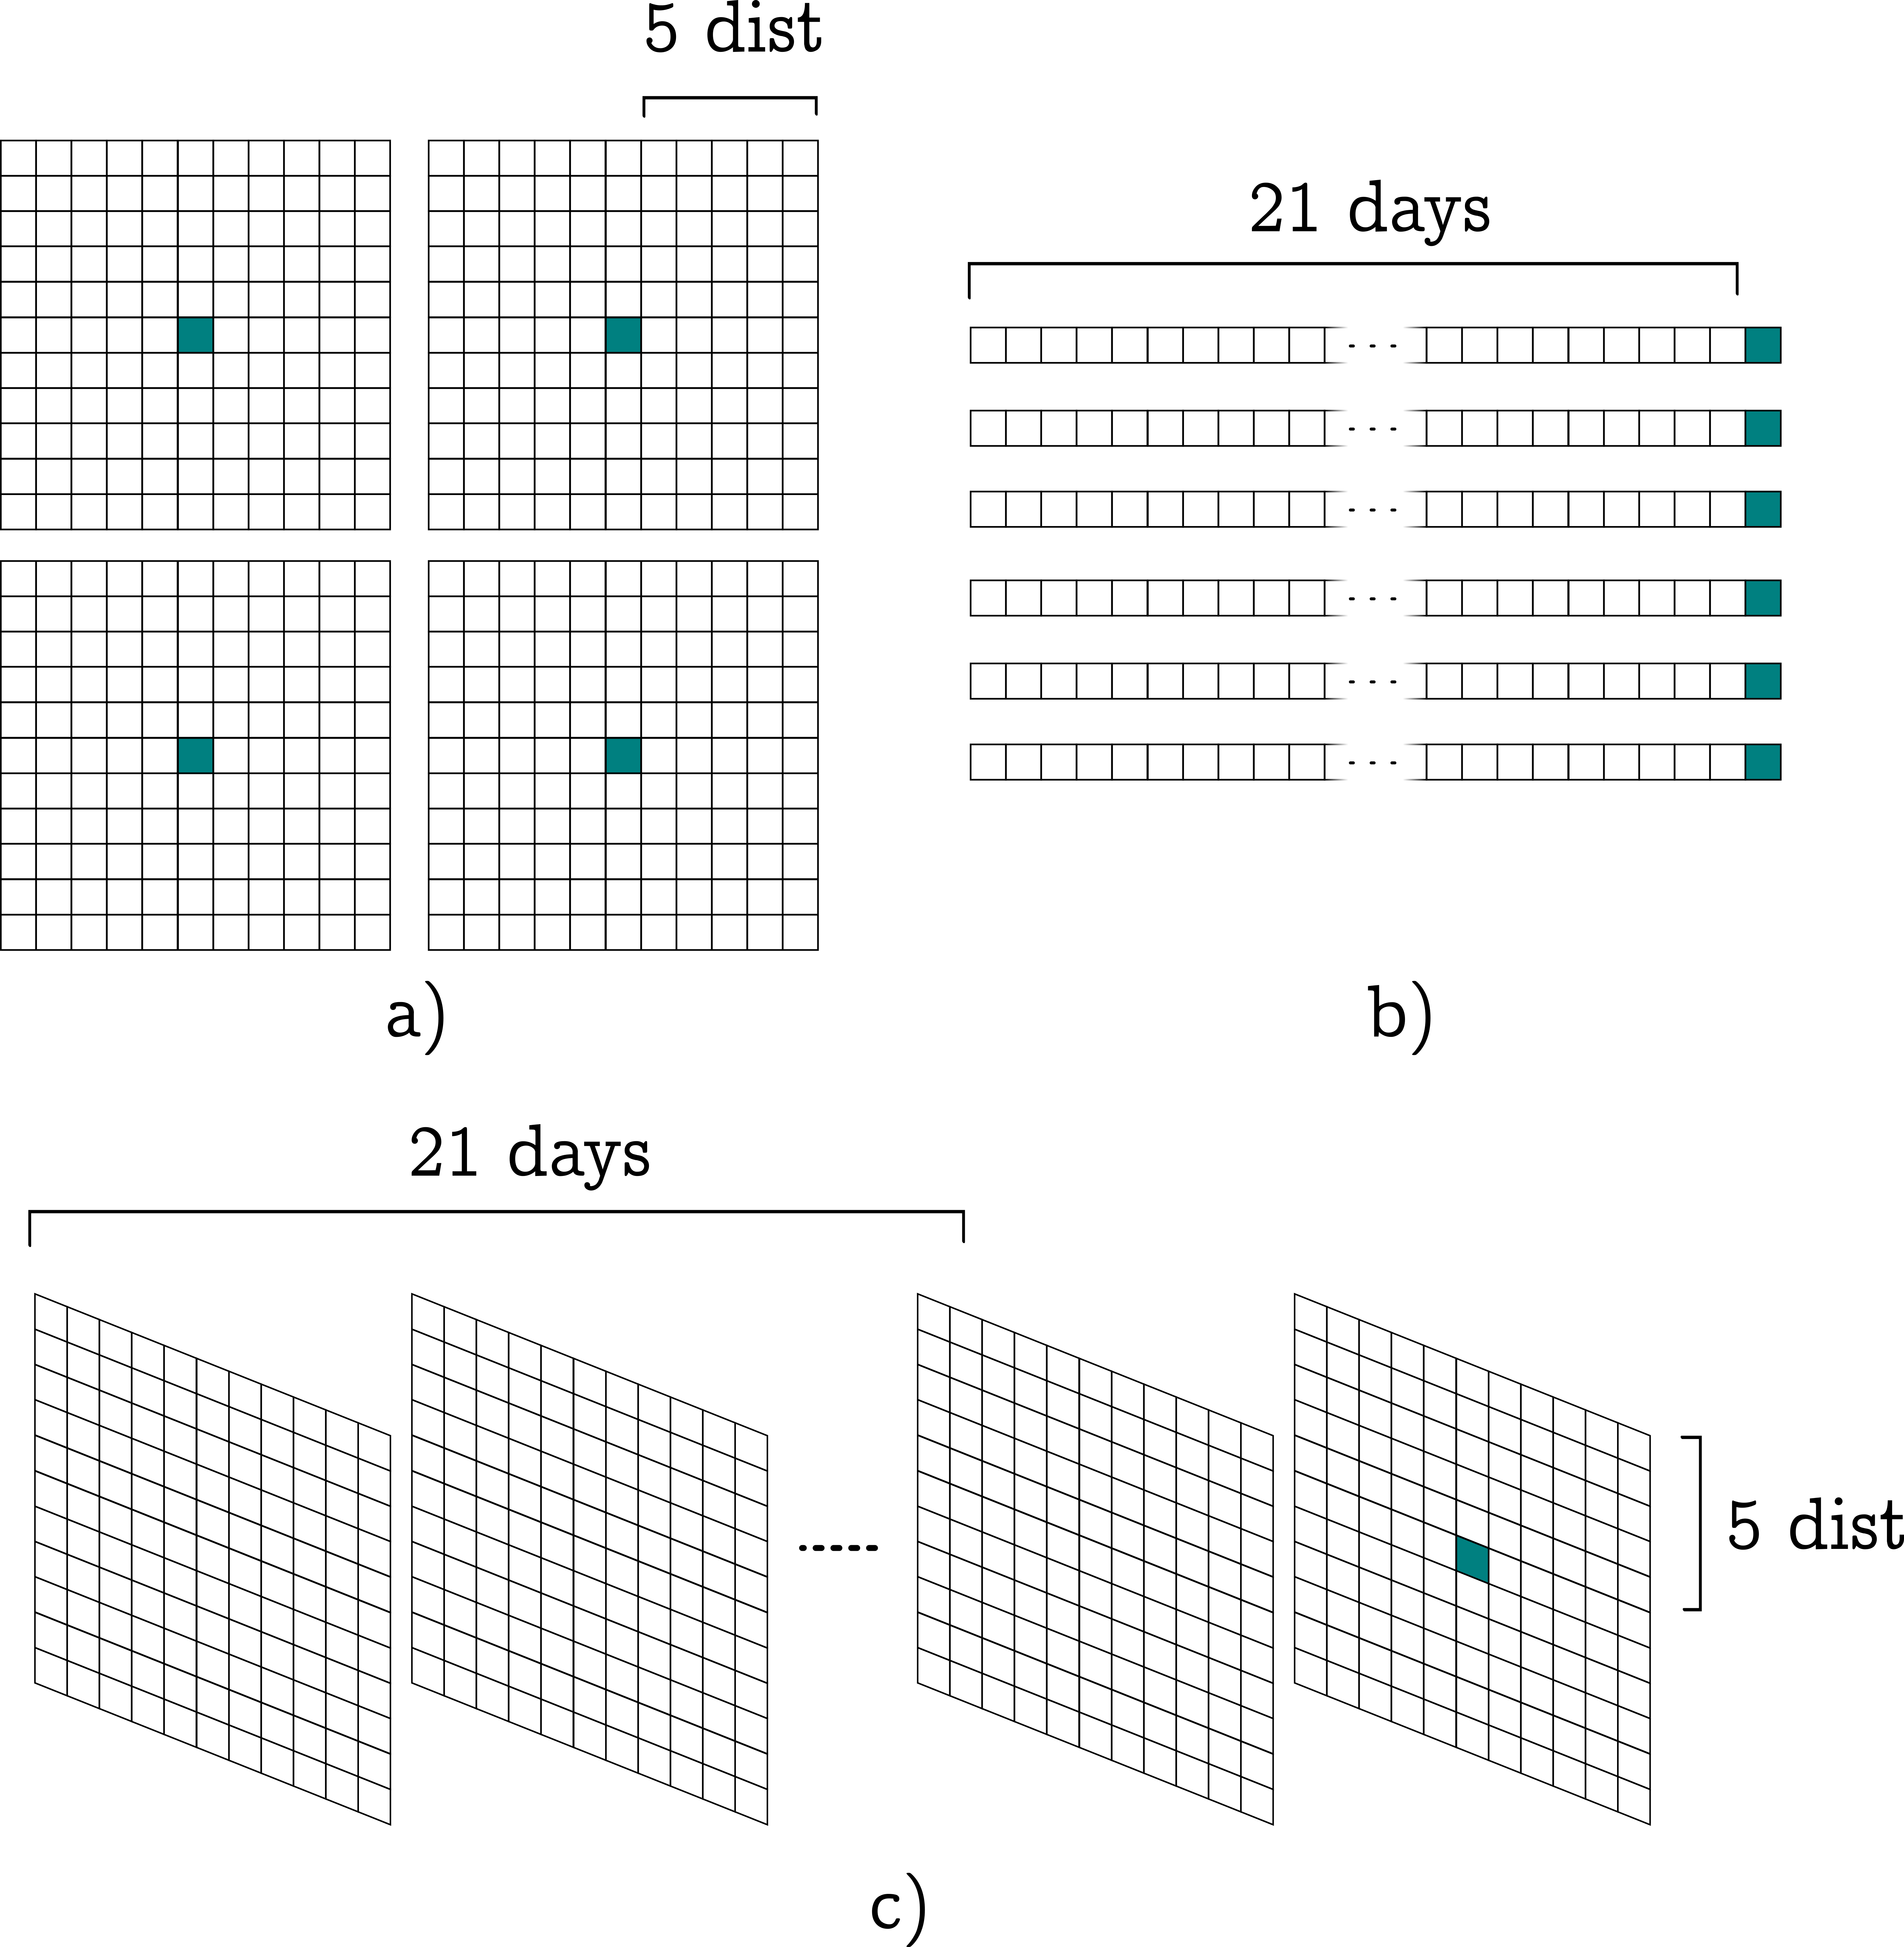
\includegraphics[scale=0.04]{data_types}\label{fig:data_types}
    \caption{Illustration of types of data -- a) example data based on place information, b) example data based on time information, c) combination of both.}
\end{figure}

\subsection{Problem definition}\label{sec:problem_definition}

After all data preparations, the dataset consists of a lot of records ($\approx1\,800\,000$ rows), but it is extremely sparse ($\approx20\,000$ positive targets). In general, there is minority of crimes which occurred during analysed time interval. There are also places where crimes frequently occurred due to convenient surroundings and places where nothing happened all the time.

To find answers to these questions, six main tasks were defined at the beginning of the analysis:

\begin{enumerate}
    \item Build \gls{rf}, \gls{gbm}, \gls{dl} models with default setting and \gls{cnn}, \gls{rnn} models with simple structure to try how accurate they are with all types of data (time information, neighbour information and combination of both). Then try to find the better setting for models to improve the accuracy of prediction.
    \item Verify which set of features are the most important and try to improve prediction using feature selection.
    \item Compare the models and select the best one.
    \item Try to improve prediction of the best model using feature extraction from \gls{cnn} or \gls{rnn}.
\end{enumerate}

To summarise, the goal is to predict if the crime will occur in particular place next day or not. The fact that a crime (it does not matter if one or more) occurred on a given day in a given location is indicated by positive label ('1') otherwise by negative label ('0'). Then this problem can be transformed into classification problem, and all mentioned predictive methods for classification can be used.

\section{Preparation of the experiments}\label{sec:preparation}

In this section metrics and evaluation methods are described, and base models are built to define a base line. Then the libraries which I used for predictive analysis are mentioned. Finally, a setting of hyperparameters of models and their notation were defined. 

\subsection{Evaluation and used metrics}
 
Metrics for model training and evaluation of predictions is essential, and it can significantly affect the results. Different metrics have to be select for training and testing of model performance. 
 
For model training, I selected various metrics which depends on a model. To train \gls{rf}, \gls{gbm}, \gls{dl}, the \gls{auc} as the stopping metric, the value 0.01 as the stopping tolerance and grid search with RandomDiscrete strategy were chosen. To train \gls{cnn}, \gls{rnn} and the combination of both, the Binary cross-entropy as loss function, the ADAM as the optimizer and Sigmoid as the activation function after the last layer were chosen. 

This problem is a binary classification because the labels (classes) are '0' or '1'. For model evaluation I used prepared test data which I described in section~\ref{sec:result_datasets}. \gls{roc} and \gls{prc} were used for the comparing models. For finding the best threshold, I chose \gls{mcc} which is based on \gls{roc} analysis and respect unbalanced data.  

After finding an optimal threshold I compute some other metrics of prediction -- \gls{acc} and \gls{f1} score. In the figure~\ref{fig:base_best_worst}(a) there is represented the best possible case on test data displayed using confusion matrix. All crimes are classified correctly and no one incorrectly -- all metrics are equal 1. In the figure~\ref{fig:base_best_worst}(b) is represented the worst case -- all metrics are zero except \gls{mcc}, which is equal -1. (This case means that every class are labelled wrong, but if it was possible to detect this situation, it is easy to invert result and get the best case -- it is only an example to demonstrate values of all used metrics in both cases, the best and the worst.) 

\begin{figure}[ht]\centering
    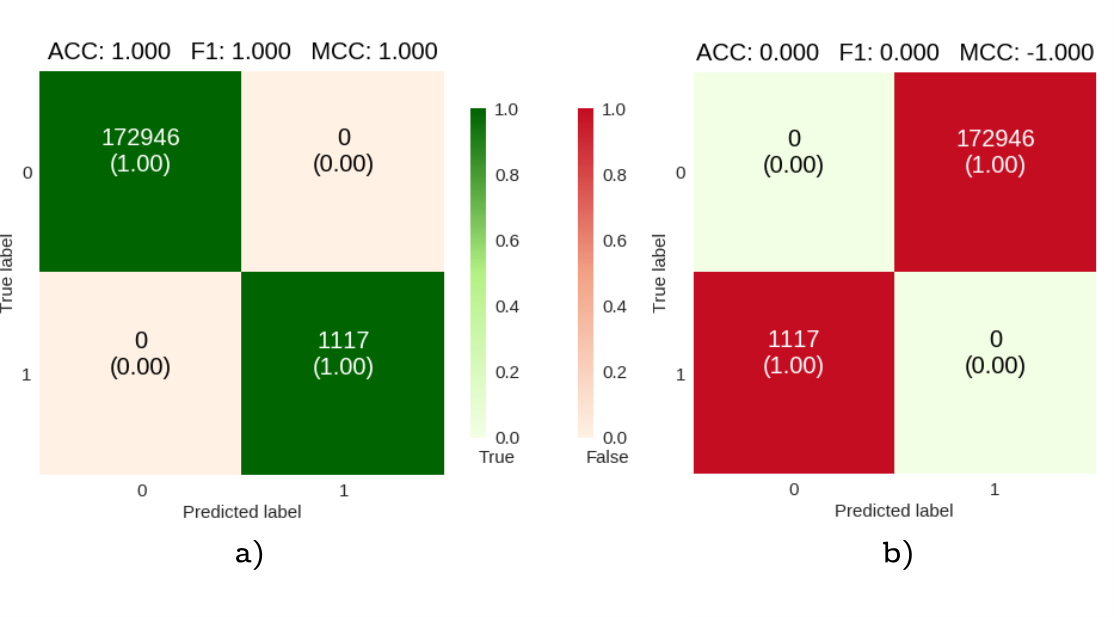
\includegraphics[scale=0.30]{cm_best_worst}
    \caption{Confusion matrix -- a) result of the best case prediction, b) result of the worst case prediction.}\label{fig:base_best_worst}
\end{figure}

To summarise, the main goal in this classification problem is to get the most correctly labelled class '1' and to minimise incorrect label for class '0', but the first is the more important. The all resulting metrics should be equal almost 1. For example, if the model predicts that a crime will occur and it will not, police officers will go to a place unnecessarily, but it is still better than do not detect crime. The main problem is that the police is not able to cover all places in the Prague to prevent a minor crime. So that, the predictive analysis is not about finding a strong and robust model but also about correct parameter and evaluation settings.

\subsection{Base models}

To set up baseline against which improvements can be measured I chose three model based on simple assumptions. First, I predict all the labels to be '0', so that no crime will not occur. The result confusion metrics of this \gls{bm} is in the figure~\ref{fig:base_zero_one}(a). The second base model is base on prediction where I predict all the labels to be '1' so that every day in every places crime will occur. The result confusion metrics is in the figure~\ref{fig:base_zero_one}(b).

The resulting confusion matrix and the \gls{acc} show, that first base model is not so bad. The \gls{acc} is almost 1, what is the great result. But \gls{f1} score is almost 0 (in the picture is 0.000 due to rounding), so that indicates not so great result because data are unbalanced and only one class (the bigger) was predicted correctly. That is why the \gls{acc} is high. The \gls{mcc} is neutral which also indicates not so good result. It means that overcome this \gls{acc} will not be so easy.

In the opposite case the \gls{acc} is almost 0 because majority of labels were incorrect predicted. But the \gls{f1} score is better than \gls{f1} of the first base model, because \gls{tp} is more important than \gls{tn} from a definition of \gls{f1} (see \ref{sec:measures}). 

\begin{figure}[ht]\centering
    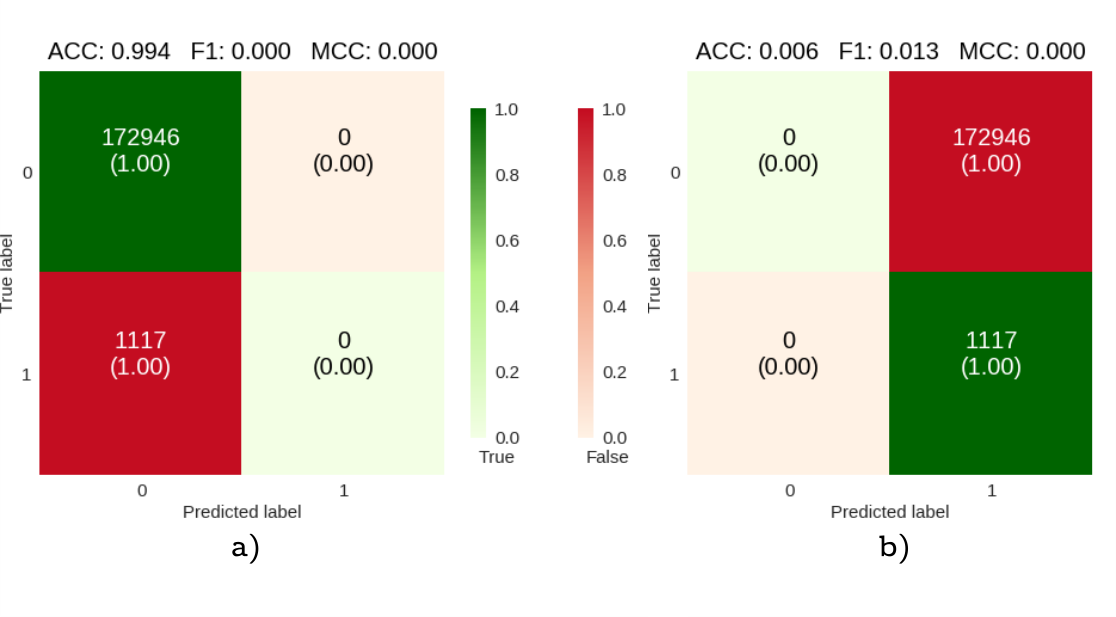
\includegraphics[scale=0.30]{cm_zero_one}
    \caption{Confusion matrix -- a) result of prediction by no crime every day in the whole area (all prediction are zero), b) result of prediction by crime every day in the whole area (all prediction are one) .}\label{fig:base_zero_one}
\end{figure}

The last base model is a bit more sophisticated. The prediction was based on the assumption that the crime will occur only if also occurred previous day in the same place. The result confusion matrix and metrics are in the figure~\ref{fig:base_prev}. The \gls{acc} is high in opposite the \gls{f1} and \gls{mcc} are still low. But it is still the best result from these three presented base models. The model predicted 24 crimes and only 1104 crimes were classified incorrectly. 

\begin{figure}[ht]\centering
    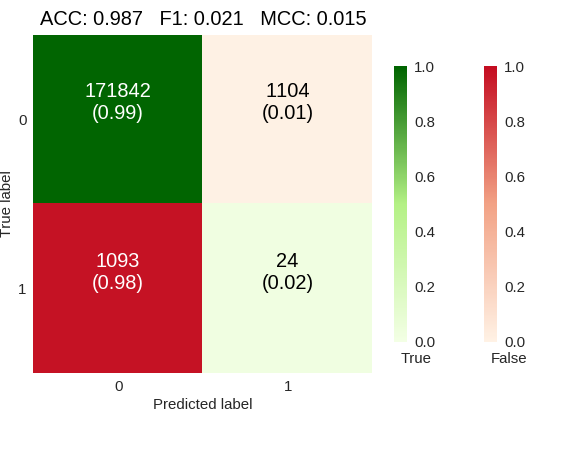
\includegraphics[scale=0.35]{cm_base_prev}
    \caption{Confusion matrix -- result of prediction by previous day.}\label{fig:base_prev}
\end{figure}

The summary all of the values from figures are in table~\ref{tab:base_summary}. As emerged from the results of base models, the best \gls{acc} is not easy to overcome, but there is still room for improvement of \gls{f1} score and \gls{mcc}.

\begin{table}[H]\centering
\begin{small}
    \caption{Summary of base models -- results from confusion matrix and selected metrics.}\label{tab:base_summary}
    \begin{tabular}{|l|c|c|c|c|c|c|c|}\hline
        Model & \gls{tn} & \gls{fn} & \gls{tp} & \gls{fp} & \gls{acc} & \gls{f1} & \gls{mcc} \tabularnewline \hline \hline
        \gls{bm} 'zero' & 172946 & 0 & 0 & 1117 & 0.994 & 0.000 & 0.000 \tabularnewline \hline
        \gls{bm} 'one' & 0 & 172946 & 1117 & 0 & 0.006 & 0.013 & 0.000 \tabularnewline \hline
        \gls{bm} 'previous day' & 171842 & 1104 & 24 & 1093 & 0.987 & 0.021 & 0.015 \tabularnewline \hline
    \end{tabular}
\end{small}
\end{table}

\subsection{Used libraries for modelling}
There is a lot of possibilities to create prediction models for many problems like scripting languages, statistic and predictive software and a big amount of libraries for many programming languages. I chose Python language and two useful and robust library for machine learning -- H2O\cite{h2o_soft} and Keras\cite{keras_soft}. All scripts related to predictive analysis is created using Python 3.4 and Jupyter notebook environment. I also used a lot of other Python libraries mostly for result evaluation and visualisation.

\subsubsection{H2O}
H2O is the open source deep learning platform written in Java. It uses in-memory compression and integrates with Hadoop and Spark products. It offers Flow graphical user interface, programming environments like R, Python, Java, Scala, JSON and also REST API. H2O includes many common machine learning algorithms. It provides Data agnostic support for all common database and file Types, massively scalable big data analysis and real-time data scoring too.\cite{h2o_ML_booklet}

The H2O is pretty easy to use. Users need not build model step by step; they select the model and tune parameters only. On the other hand, users can not change the model's structures. They can also build own ensembles. The H2O team provide a lot of materials and examples to use. There is also a huge user's community and support.\cite{h2o_ML_booklet} A simple example of code is in listing~\ref{code:h2o}.


\begin{listing}
\begin{scriptsize}
\begin{minted}{python}
import h2o
from h2o.estimators.gbm import H2OGradientBoostingEstimator

h2o.init()

model = H2OGradientBoostingEstimator(distribution='bernoulli',
                                     ntrees=100,
                                     max_depth=4,
                                     learn_rate=0.1)

model.train(x=x,
            y=y, 
            training_frame=train,
            validation_frame=validation)
            
perf = model.model_performance(test)
auc = perf.auc()
prediction = predict(test)
\end{minted}
\caption{Simple example of using H2O in Python.}
\label{code:h2o}
\end{scriptsize}
\end{listing}


I was interested in Python H2O modul. I used \gls{drf} (\texttt{H2O\-Ran\-dom\-Forest\-Esti\-ma\-tor}), \gls{gbm}  (\texttt{H2O\-Gradient\-Boosting\-Esti\-ma\-tor}) and \gls{dl} (\texttt{H2O\-Deep\-Lear\-ning\-Esti\-ma\-tor}) models and module for grid search (\texttt{H2O\-Grid\-Search}). 

\subsubsection{Keras}
Keras is library focusing on neural networks written in Python. It is a model-level library, which provides high-level building blocks for developing deep learning models, and therefore users can use Python and TensorFlow (an open-source symbolic tensor manipulation framework developed by Google) or Theano (an open-source symbolic tensor manipulation framework developed by LISA/MILA Lab at Université de Montréal) backend.

The Keras is also user-friendly and easy to use. Users can build both \gls{rnn} and \gls{cnn} as well as combinations of the two and they can run the code on \gls{cpu} or \gls{gpu}. A simple example of code is in listing~\ref{code:keras}.

\begin{listing}
\begin{scriptsize}
\begin{minted}{python}
from keras.models import Sequential
from keras.layers import Dense, Activation

model = Sequential()

model.add(Dense(units=64, input_dim=100))
model.add(Activation('relu'))
model.add(Dense(units=10))
model.add(Activation('softmax'))

model.compile(loss='categorical_crossentropy',
                  optimizer='sgd',
                  metrics=['accuracy'])
              
model.fit(x_train,
              y_train, 
              epochs=5, 
              batch_size=32)
          
loss_and_metrics = model.evaluate(x_test, y_test)                      
prediction = model.predict(x_test)  
\end{minted}
\caption{Simple example of using Keras in Python.}
\label{code:keras}
\end{scriptsize}
\end{listing}

I used Keras with the combination of Theano backend to build predictive models contained \gls{cnn}, \gls{rnn} layers and other useful layers for building \gls{nn} such as Activation (\gls{relu}, Sigmoid), Dropout and Dense layers. I could use DeepWater\cite{h2o_deepwater} module from H2O based on TensorFlow to build models similar way, but I wanted to try another platform than H2O.

\subsection{Selection of predictive methods}

For predictive analysis, I selected several nontrivial predictive methods -- Random Forest, Gradient Boosting Machines, Deep learning, Convolution Neural Network and Recurrent Neural Network to compare generalisation success with real crime data. 

\gls{rf} and \gls{gbm} both based on decision trees are good predictors in general for unbalanced data too. \gls{ann} can solve a variety of problems. There are a lot of modifications of standard \gls{ann} such as \gls{dl} which used a lot of layers of neurones for generalisation of the problem, \gls{cnn} which can solve image based problems and \gls{rnn} which used memory to learn from time-based problems. I examined all of these properties on real crime data.

During the experiment, I inspected all mentioned predictive methods on each type of data separately. Using different methods, I tested several models and then I selected the best. Finally, I compared results from all methods for each type of data and select the best one. 

\subsubsection{H2O parameters}
I used H2O library to train \gls{rf}, \gls{gbm} and \gls{dl} models. First I trained models with default parameter setting to inspect how these algorithms predict in general. Then I tried to find the best model setting using grid search. For comparison, I select three best models from all methods.

Setting for grid search for all models was strategy 'RandomDiscrete', stopping metric \gls{auc}, stopping tolerance 0.01 and stopping rounds 5.

The set of parameters and default setting of \gls{rf} algorithm are described in documentation\cite{h2o_drf_doc}. As the hyperparameters for grid search, I selected a number of trees (20, 40, 50, 70, 90, 100 and 150) and maximal depth (5, 10, 30, 50 and 100). In the summary of models, these model have names DRF\_default or DRF\_i\_j where i is the i-th index of a number of tree parameter setting, and j is the j-th index of maximal depth parameter setting ( the first index is 1). I also set minimal rows in leafs to 20.

The set of parameters and default setting of \gls{gbm} algorithm are described in documentation\cite{h2o_gbm_doc}. As the hyperparameters for grid search, I selected a number of trees (20, 30, 40, 50, 60, 70) and maximal depth (5, 10, 30, 50). In the summary of models, these models have names GBM\_default or DRF\_i\_j where i is the i-th index of a number of tree parameter setting, and j is the j-th index of maximal depth parameter setting. I also set minimal rows in leafs to 20.

The set of parameters and default setting of \gls{dl} the algorithm are described in documentation\cite{h2o_dl_doc}. As the hyperparameters for grid search I selected number of hidden layers and neurons ([100, 100], [512],[16, 16, 16, 16, 16],[32, 32, 32, 32, 32], [64, 64, 64]) and input dropout rations (0.2, 0.3, 0.4). In the summary of models, these models have names DEL\_default or DEL\_i\_j where i is i-th index of hidden layers and neurons parameters and j is j-th index of input dropout ration parameter setting. I also set l1 to 0.0001, l2 to 0.0001 and score validation sampling to 'Stratified'.

\subsubsection{Keras parameters}
I built \gls{cnn} and \gls{rnn} models using Keras library and the process of building model was a bit different. I built all models layer by layer, and I searched for the best structure and parameter settings together. I had to also modify a structure of data. 

As an input into \gls{cnn}, I used information about crime count in the neighbourhood the day before observed place and time and transformed it from the vector into the array. The \gls{cnn} tried to learn this information from the array as from an image to find some patterns and based on this to make a good prediction. In the summary of models, these models have name CNN\_f\_l where f is a number of filters in each layer and l is number of layers.

The \gls{rnn} has as an input sequence of data. I tried to learn the \gls{rnn} to find some patterns in 21 days long time series to predict if crime will occur or not. I used \gls{lstm} neurones only. In the summary of models, these models have names RNN\_n\_l where n is a number of neurones in each layer and l is a number of layers. 

Finally, I combined \gls{cnn} and \gls{rnn} (time and neighbour data) together and inspected the best model structure, parameter settings and if the prediction was improved. In the summary of models, these model have names CRNN\_f\_l1\_n\_l2 f is some filters in each convolution layer, l1 is a number of convolution layers, n is a number of neurones in each recurrent layer, and l2 is a number of recurrent layers. The data for this task have to be different. The input format is (x,21,11,11) because the training was using timesteps with size 21 days and size of images is 11 $\times$ 11. So the data were split into training (1\,199\,352 rows), validation (327\,096 rows) and test (190\,806 rows) parts to respect these format and chronological order of data.

\section{Predictive analysis and evaluation}

This section is about experiments which were made with crime data from part of Prague city. The accuracy of models which I created with all three types of data (described in section~\ref{sec:preprocessing}) was evaluated, and several improvements were tried. Finally, the results were evaluated, compared and discussed.

Based on each type of data, the best models of each algorithm are selected according to sorting selected metrics -- the first by \gls{auc}, then, by \gls{mcc} and finally by \gls{tp}. All these result model are compared together using \gls{roc} and \gls{prc} curves. The every \gls{roc} and \gls{prc} plot in this section are cut, due to unbalanced data, so only the most interesting parts are displayed -- \gls{roc} x-axis and y-axis are from 0 to 0.6 and \gls{pcr} x-axes is from 0 to 0.5 and y-axes from 0 to 0.2. Finally, the completely \gls{roc} analysis and feature importance the best model is shown.

\subsection{Data with time information}\label{sec:tm_information}

The first observed type of data were data with time information. It means the explanatory variables were the base information from the source database, localisation, parsed date and extracted time features) and associated time series 21 days long into the past, except the \gls{rnn} method, where I used only time series.  

In the table~\ref{tab:tm_data_summary}, you can see the best models of each algorithm. The \gls{drf} model is best -- with defined \gls{mcc} threshold was able to predict 471 crimes correctly, on the other hand 27\,233 crimes detected in places, where crime did not occurred (see also figure~\ref{fig:roc_tm_data_best}). 

\vspace*{0.2cm}
\begin{table}[H]\centering
\begin{small}
    \caption{Summary of best models of each algorithm trained on time data -- results from confusion matrix and selected metrics.}\label{tab:tm_data_summary}
    \begin{tabular}{|l|c|c|c|c|c|c|c|c|}\hline
        Model & \gls{tn} & \gls{fn} & \gls{tp} & \gls{fp} & \gls{auc} & \gls{acc} & \gls{f1} & \gls{mcc} \tabularnewline \hline \hline
        DRF\_6\_3 & 145\,713 & 27\,233 & 471 & 646 & 0.701 & 0.840 & 0.033 & 0.058 \tabularnewline \hline
        GBM\_6\_1 & 163\,082 & 9\,864 & 252 & 865 & 0.700 & 0.938 & 0.045 & 0.058 \tabularnewline \hline
        DEL\_1\_3 & 168\,734 & 4\,212 & 124 & 993 & 0.679 & 0.970 & 0.045 & 0.044 \tabularnewline \hline
        RNN\_2\_100 & 172\,419 & 526 & 47 & 1\,071 & 0.589 & 0.991 & 0.056 & 0.054 \tabularnewline \hline
    \end{tabular}
\end{small}
\end{table}
\vspace*{0.2cm}

In the figure~\ref{fig:roc_tm_data_all} is comparison of all models using \gls{roc} and \gls{prc} analysis and you can see, although the \gls{rnn} is the worst based on metrics and \gls{roc} analysis, but in \gls{prc} analysis is based on \gls{rec} between 0.1 and 0.2 the best. It because the \gls{rnn} model has low \gls{fpr} at the beginning of threshold range but unfortunately also low \gls{tp}.   


\begin{figure}[ht]\centering
    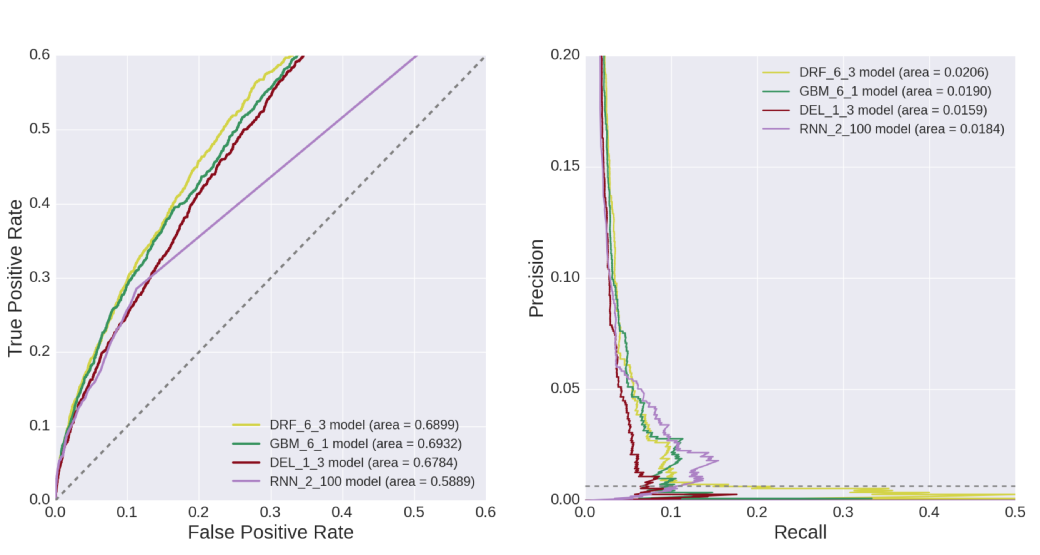
\includegraphics[scale=0.33]{roc_tm_data_all}\label{fig:roc_tm_data_all}
    \caption{\gls{roc} and \gls{prc} curves of the best models of each algorithm trained on time data.}
\end{figure}

The best \gls{drf} model's parameters are number of trees = 100 and maximal tree depth = 30. The most important features (see the figure~\ref{fig:tm_data_fi}) are Week and Weekday. Also, distance from points of interest are very important. The most important day from history is Day\_7 which means 15 days before the crime occurred. The time series data are in this case less important than the date and localisation data. 

\begin{figure}[ht]\centering
    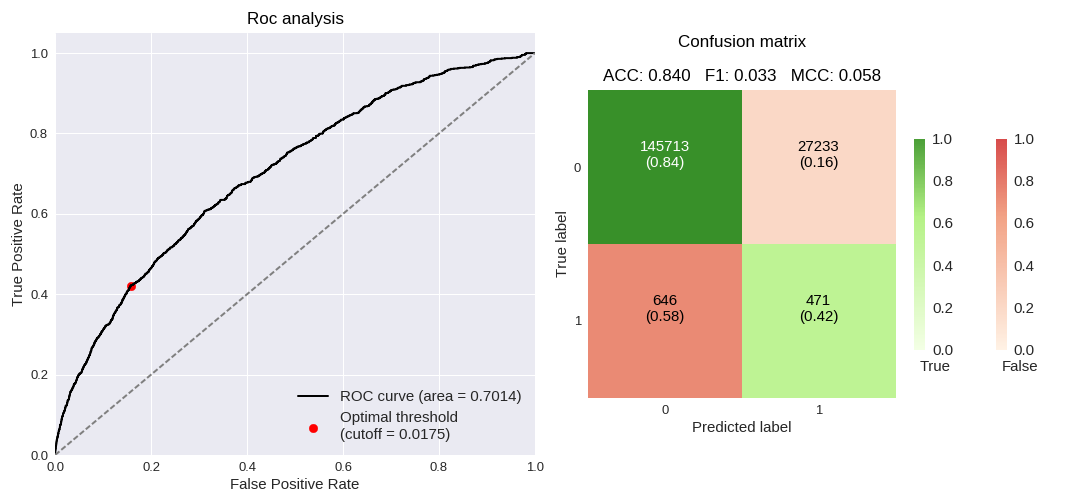
\includegraphics[scale=0.33]{roc_tm_data_best}\label{fig:roc_tm_data_best}
    \caption{Complete \gls{roc} analysis of the best model trained on time data.}
\end{figure}

\begin{figure}[ht]\centering
    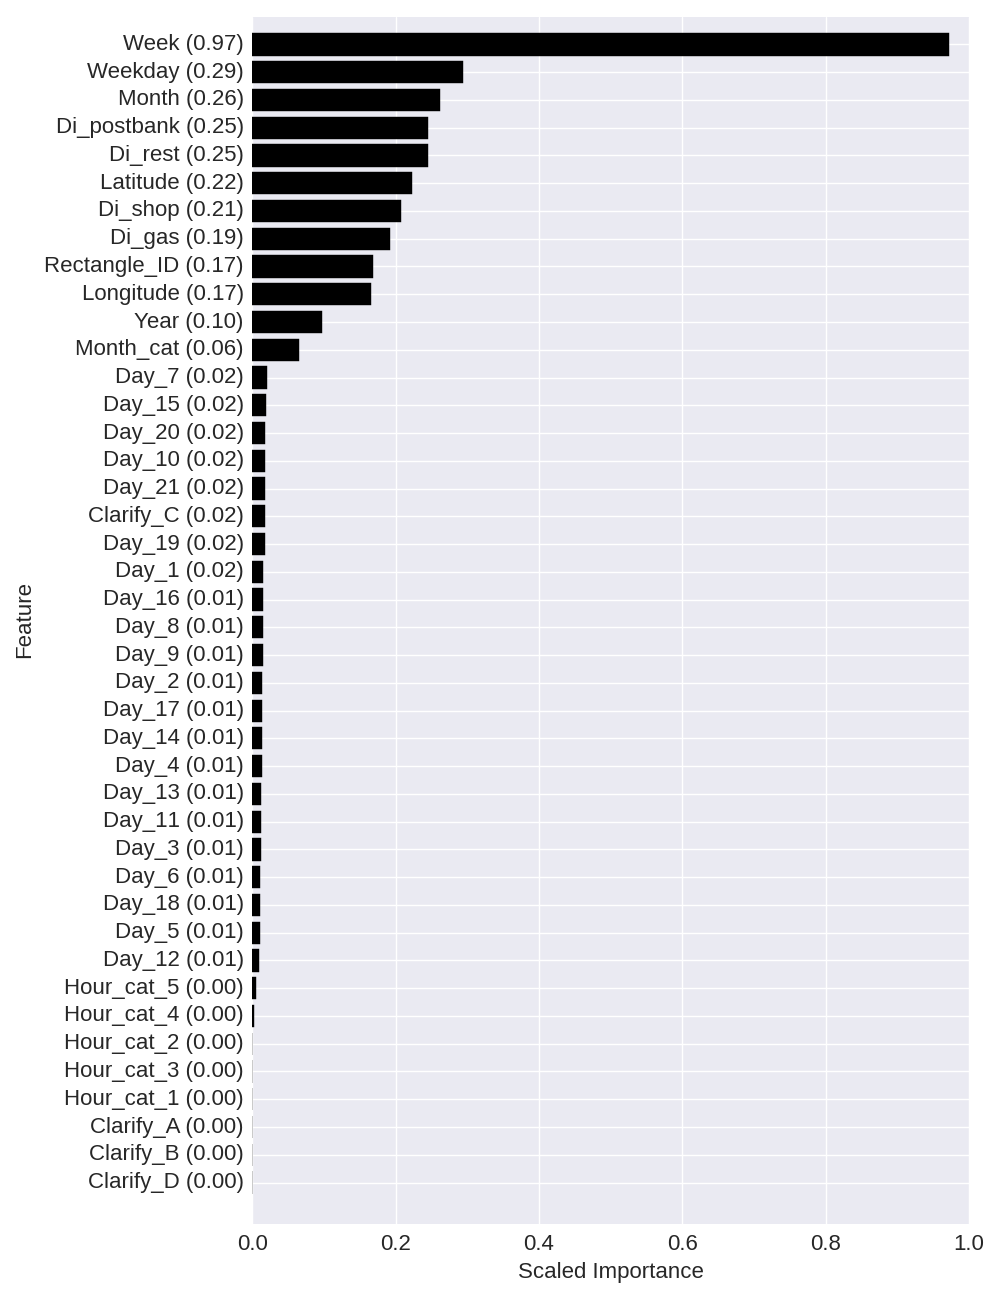
\includegraphics[scale=0.3]{tm_data_fi}\label{fig:tm_data_fi}
    \caption{Feature importance of the best model trained on time data -- the first 42 features only.}
\end{figure}

\newpage
\subsection{Data with neighbours information}\label{sec:neigh_information}

The second observed type of data were data with neighbour information. It means the explanatory variables were the base information from source database again, and associated neighbour data (121 values) the date before the crime occurred, except the \gls{cnn} method, where I used only neighbour data.  

In the table~\ref{tab:neigh_data_summary}, you can see the best models of each algorithm. The \gls{drf} model is the best again which was able to predict 289 crimes correctly with defined \gls{mcc} threshold. On the other hand 10\,403 crimes detected in places, where crime did not occur. The \gls{mcc} score is better than with time data, but the number of corrected predicted crime is slower. You can also see, that \gls{auc} is a bit higher than with time data (see also figure~\ref{fig:roc_neigh_data_best}).

The figure~\ref{fig:roc_tm_neigh_data_all} shows more consistent result of each model with neighbour data then with time data. The \gls{drf} model is the best in the both \gls{roc} and \gls{prc} analysis. The \gls{roc} analysis also shows, that \gls{cnn} model is definitely the worst, but the \gls{prc} analysis shows, that it is bad similarly to \gls{dl} model. 

\begin{table}[H]\centering
\begin{small}
    \caption{Summary of models of each algorithm trained on neighbours data -- results from confusion matrix and selected metrics.}\label{tab:neigh_data_summary}
    \begin{tabular}{|l|c|c|c|c|c|c|c|c|}\hline
        Model & \gls{tn} & \gls{fn} & \gls{tp} & \gls{fp} & \gls{auc} & \gls{acc} & \gls{f1} & \gls{mcc} \tabularnewline \hline \hline
        DRF\_7\_4 & 162\,543 & 10\,403 & 289 & 828 & 0.711 & 0.935 & 0.049 & 0.066 \tabularnewline \hline
        GBM\_default & 168\,222 & 47\,24 & 170 & 947 & 0.697 & 0.967 & 0.057 & 0.060 \tabularnewline \hline
        DEL\_default & 114\,700 & 58\,246 & 650 & 467 & 0.650 & 0.663 & 0.022 & 0.041 \tabularnewline \hline
        CNN\_2\_64 & 142\,277 & 30\,669 & 341 & 776 & 0.590 & 0.819 & 0.021 & 0.027 \tabularnewline \hline
    \end{tabular}
\end{small}
\end{table}

\begin{figure}[ht]\centering
    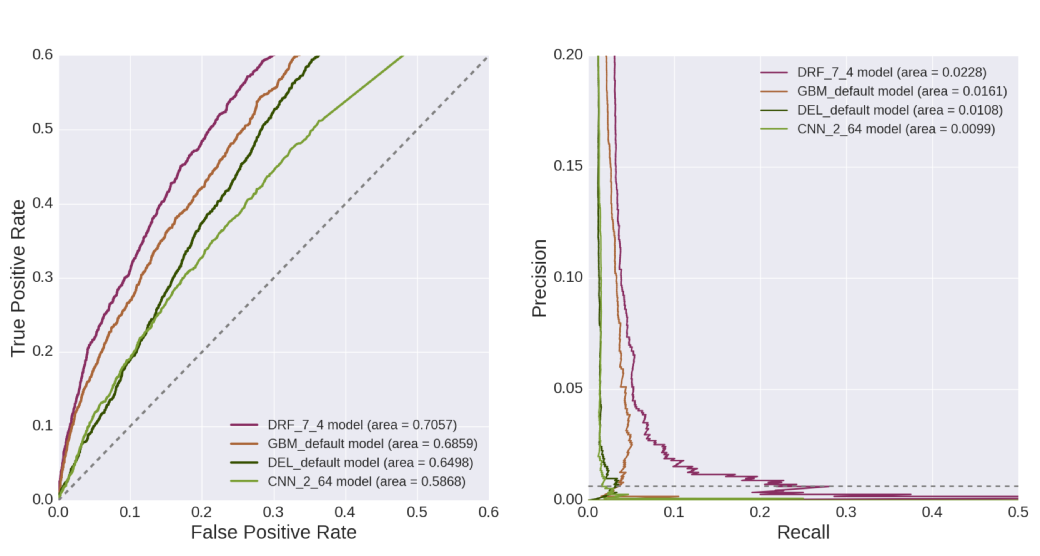
\includegraphics[scale=0.33]{roc_neigh_data_all}\label{fig:roc_neigh_data_all}
    \caption{\gls{roc} and \gls{prc} curves of the best models of each algorithm trained on neighbours data.}
\end{figure}

\begin{figure}[ht]\centering
    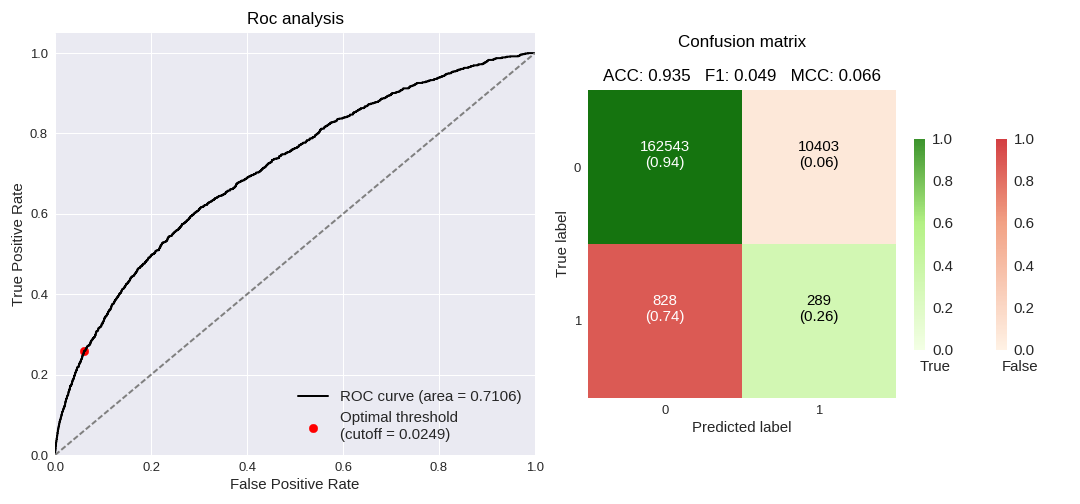
\includegraphics[scale=0.33]{roc_neigh_data_best}\label{fig:roc_neigh_data_best}
    \caption{Complete \gls{roc} analysis of the best model trained on neighbours data.}
\end{figure}

The best \gls{drf} model's parameters are number of trees = 150 and maximal tree depth = 50. The most important features (see the figure~\ref{fig:neigh_data_fi}) are Day and Di\_post\_bank. Again the important are also other distances from points of interest and date information. From neighbour, information is the most important Neigh\_60, what is exactly the day before date where the crime occurred. The other most important neighbours are these that are near the area, where the crime occurred. 

\begin{figure}[ht]\centering
    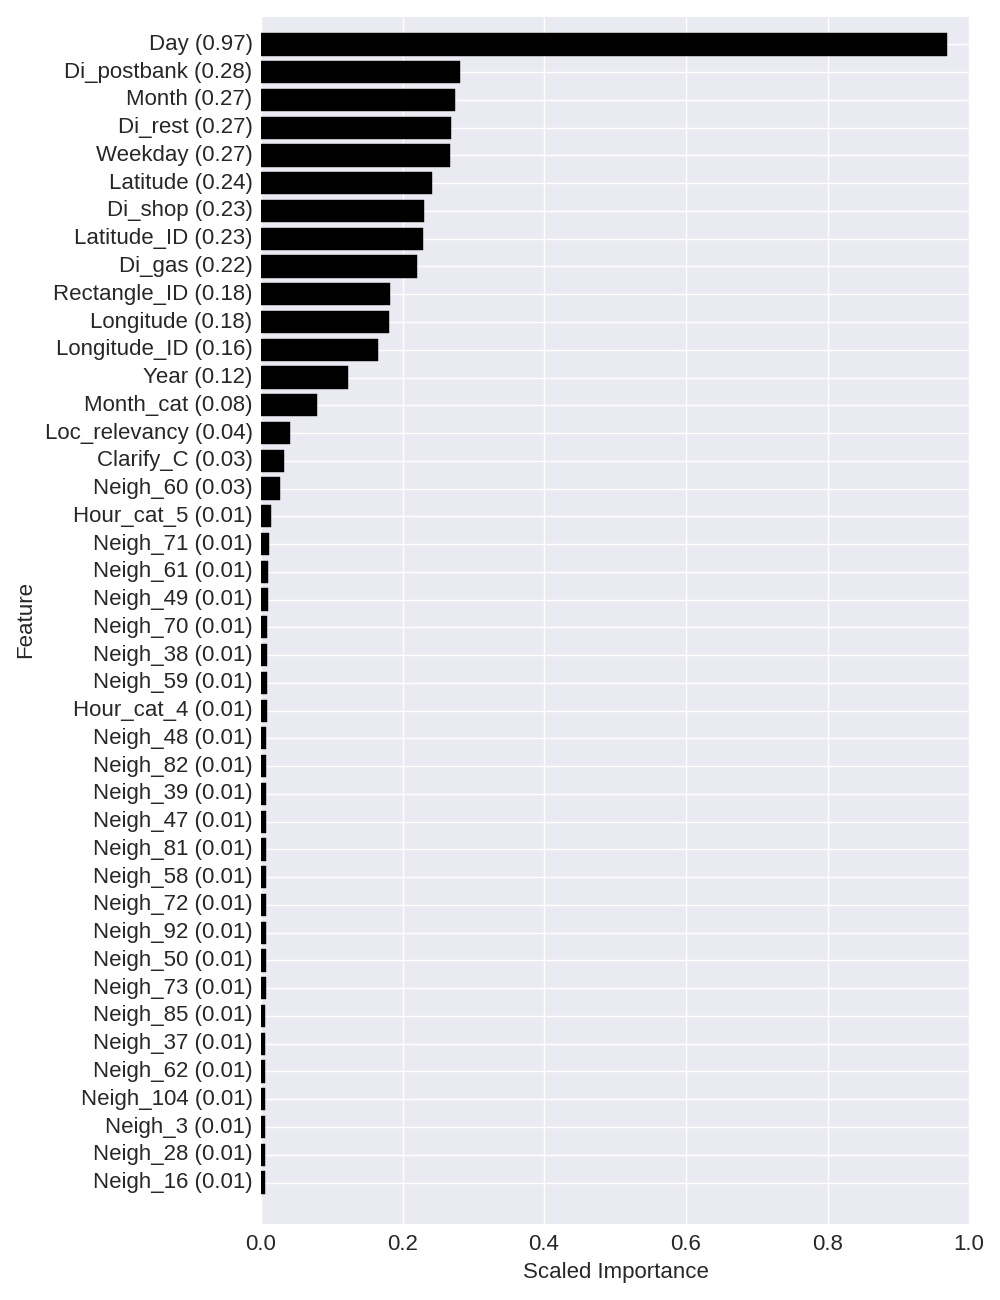
\includegraphics[scale=0.3]{neigh_data_fi}\label{fig:neigh_data_fi}
    \caption{Feature importance of the best model trained on neighbours data -- the first 42 features only.}
\end{figure}

\subsection{Combination time and neighbour information}\label{sec:tm_neigh_information}

The last type of data is the combination of both time and neighbour information and also with data from the database. It can be expected, that combination of all data bring the best solution. 

In the table~\ref{tab:neigh_data_summary} you can see the best models of each algorithm. For the third time, the best model is \gls{drf} model and in this case, the result of the best model is distinctly better than other results. The \gls{mcc} threshold keep the \gls{fpr} low, so only 298 crimes were corrected predicted and \gls{fn} are higher than with neighbour data, on the other hand \gls{auc} is the highest achieved (see also figure~\ref{fig:roc_tm_neigh_data_best}).

\begin{table}[H]\centering
\begin{small}
    \caption{Summary of models of each algorithm trained on a combination time and neighbours data -- results from confusion matrix and selected metrics.}\label{tab:tm_neigh_data_summary}
    \begin{tabular}{|l|c|c|c|c|c|c|c|c|}\hline
        Model & \gls{tn} & \gls{fn} & \gls{tp} & \gls{fp} & \gls{auc} & \gls{acc} & \gls{f1} & \gls{mcc} \tabularnewline \hline \hline
        DRF\_6\_5 & 161\,733 & 11\,213 & 298 & 819 & 0.716 & 0.931 & 0.047 & 0.065 \tabularnewline \hline
        GBM\_6\_1 & 166\,687 & 6\,259 & 213 & 904 & 0.701 & 0.959 & 0.056 & 0.065 \tabularnewline \hline
        DEL\_5\_3 & 158\,443 & 14\,503 & 266 & 851 & 0.672 & 0.912 & 0.033 & 0.044 \tabularnewline \hline
        CRNN\_2\_8\_1\_100 & 130\,371 & 59\,189 & 699 & 547 & 0.669 & 0.687 & 0.023 & 0.043 \tabularnewline \hline
    \end{tabular}
    \end{small}
\end{table}

In this case, the result \gls{roc} and \gls{prc} curves of \gls{drf} and \gls{gbm} are mostly close to each other (see figure~\ref{fig:roc_neigh_data_all}). But the random principal of \gls{rf} model again better generalised. Interesting is, despite the model based on combination of \gls{cnn} an \gls{rnn} was trained only with neighbour and time information from data, has similar result with the \gls{dl} model and in some parts of \gls{roc} plot is even better. 

\begin{figure}[ht]\centering
    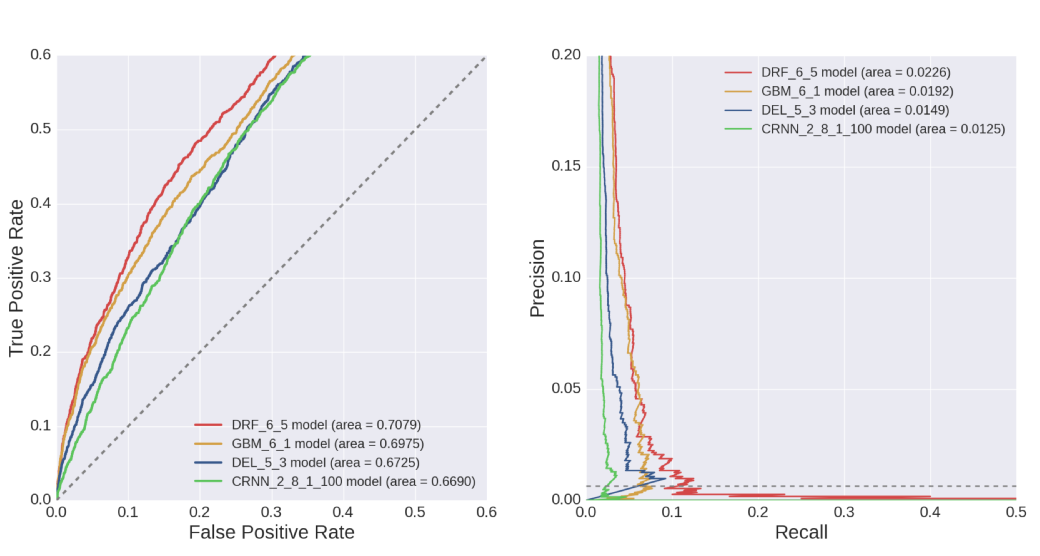
\includegraphics[scale=0.33]{roc_tm_neigh_data_all}\label{fig:roc_tm_neigh_data_all}
    \caption{\gls{roc} and \gls{prc} curves of the best models of each algorithm trained on a combination time and neighbours data.}
\end{figure}

\begin{figure}[ht]\centering
    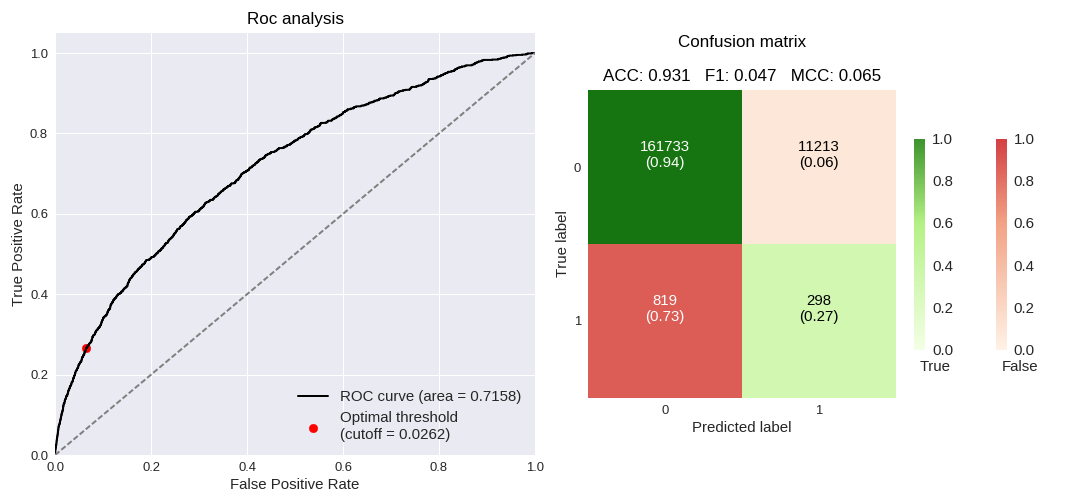
\includegraphics[scale=0.33]{roc_tm_neigh_data_best}\label{fig:roc_tm_neigh_data_best}
    \caption{Complete \gls{roc} analysis of the best model trained on a combination time and neighbours data.}
\end{figure}

\begin{figure}[ht]\centering
    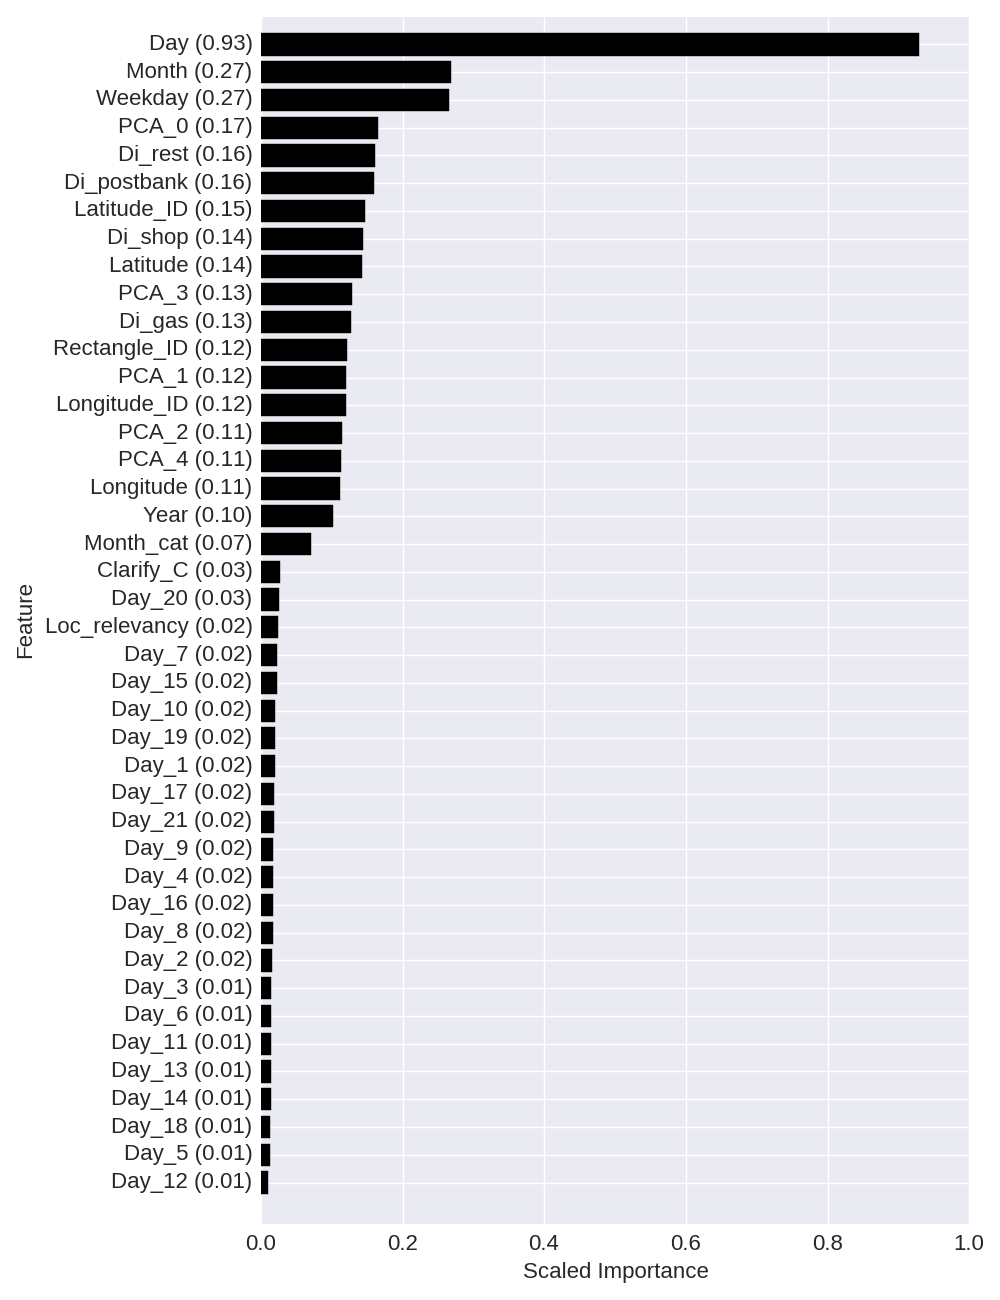
\includegraphics[scale=0.3]{tm_neigh_data_fi}\label{fig:tm_neigh_data_fi}
    \caption{Feature importance of the best model trained on a combination time and neighbours data -- the first 42 features only.}
\end{figure}

The best \gls{drf} model's parameters are number of trees = 100 and maximal tree depth = 100. It is clear that with more features the maximal depth of the tree is also higher. The most important feature (see the figure~\ref{fig:tm_neigh_data_fi}) is unambiguously Day. Again, the distances from points of interest are significant. The significant are components from \gls{pca} and information from the database, after that, the close neighbours are important.


\subsection{Data selected using feature selection methods}

The last observed type of data were data with selected features using feature selection method (see section~\ref{sec:feature_selection}) from all data. The goal was to obtain if the feature selection from the whole dataset can improve the prediction. 

In the table~\ref{tab:neigh_data_summary} you can see the best models of algorithms, where feature selection was possible to try. Again the result rank is the same -- the best is \gls{drf} model, which predicted 328 crimes correctly and 13\,702 crimes detected in places, where crime did not occur (see the figure~ \ref{fig:roc_fs_data_best}). 

\begin{table}[ht]\centering
\begin{small}
    \caption{Summary of models of each algorithm trained on a combination time and neighbour data -- results from confusion matrix and selected metrics.}\label{tab:fs_data_summary}
    \begin{tabular}{|l|c|c|c|c|c|c|c|c|}\hline
        Model & \gls{tn} & \gls{fn} & \gls{tp} & \gls{fp} & \gls{auc} & \gls{acc} & \gls{f1} & \gls{mcc} \tabularnewline \hline \hline
        DRF\_5\_3 & 159\,244 & 13\,702 & 328 & 789 & 0.715 & 0.917 & 0.043 & 0.063 \tabularnewline \hline
        GBM\_4\_2 & 169\,625 & 3\,321 & 127 & 990 & 0.699 & 0.975 & 0.056 & 0.054 \tabularnewline \hline
        DEL\_5\_3 & 145\,485 & 27\,461 & 412 & 705 & 0.678 & 0.838 & 0.028 & 0.046 \tabularnewline \hline
    \end{tabular}
\end{small}
\end{table}

The disappointment is that it is not the best-achieved result. On the other hand, it is the second best result from all tried models after the \gls{drf} model trained with all data. The size of the dataset was reduced from 183 to 42 features, and the result is almost the same. The comparison of models using \gls{roc} and \gls{prc} analysis is in the figure~\ref{fig:roc_fs_data_all}.

\begin{figure}[ht]\centering
    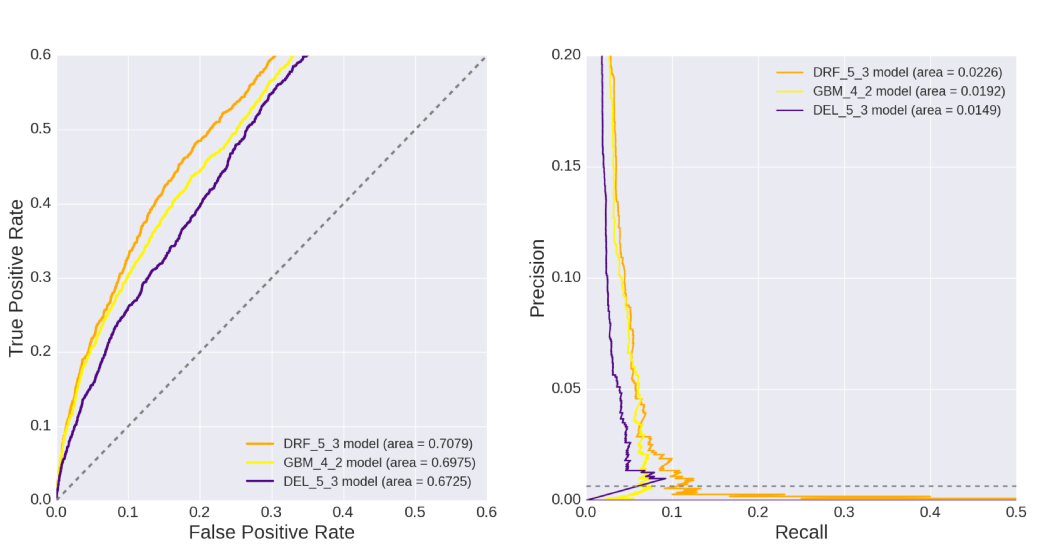
\includegraphics[scale=0.32]{roc_fs_data_all}\label{fig:roc_fs_data_all}
    \caption{\gls{roc} and \gls{prc} curves of the best models of each algorithm trained on a data selected using feature selection methods.}
\end{figure}

\begin{figure}[ht]\centering
    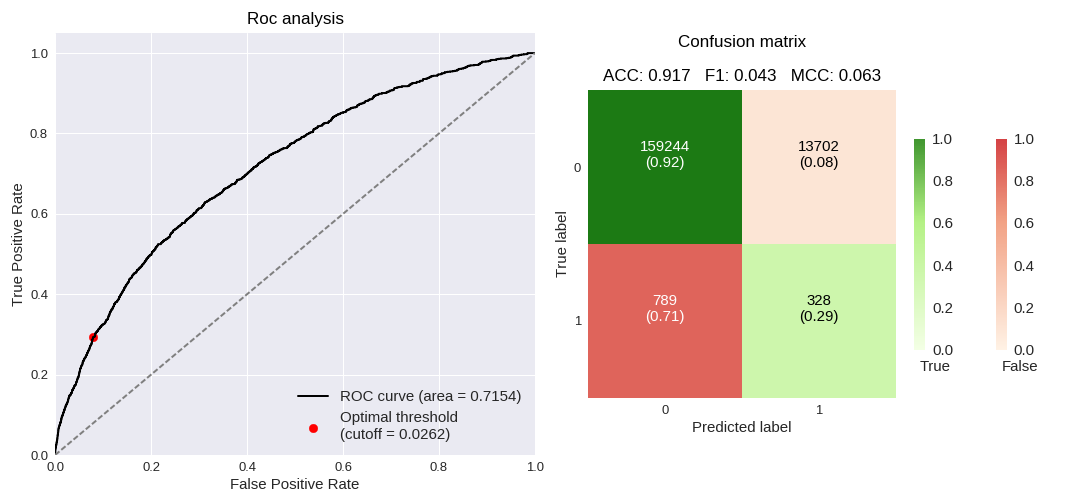
\includegraphics[scale=0.32]{roc_fs_data_best}\label{fig:roc_fs_data_best}
    \caption{Complete \gls{roc} analysis of the best model trained on a data selected using feature selection methods.}
\end{figure}

The best \gls{drf} model's parameters are number of trees = 90 and maximal tree depth = 30. The most important features (see the figure~\ref{fig:fs_data_fi}) are Weekday, components from \gls{pca} and distances from points of interest. From time information the Day\_7 is again important, and other days are useful as well.  

\begin{figure}[ht]\centering
    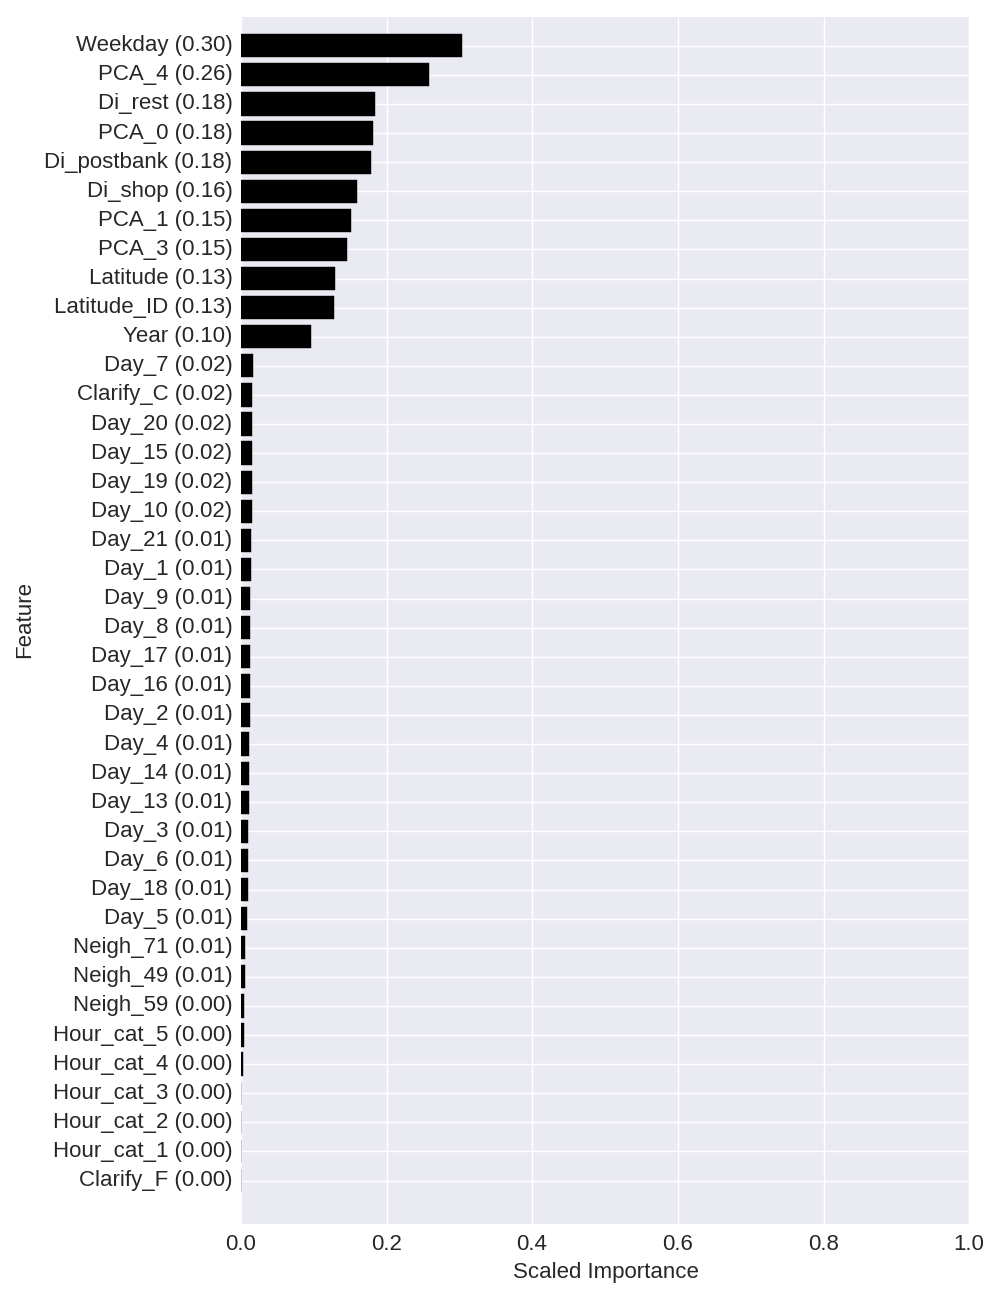
\includegraphics[scale=0.3]{fs_data_fi}\label{fig:fs_data_fi}
    \caption{Feature importance of the best model trained on a data selected using feature selection methods.}
\end{figure}

\subsection{Feature extraction using \gls{cnn} and \gls{rnn}}

The last experiment was based on the idea to use a combination of \gls{cnn} and \gls{rnn} model not for prediction, but for other feature extraction. The \gls{rnn} and \gls{cnn} models did not achieve such good result as models from H2O. If there were combined, the result was better but still inadequate. 

The best model based on \gls{cnn} and \gls{rnn} was model CRNN\_2\_8\_1\_100 (2 \gls{cnn} layers, 8 filters in each \gls{cnn} layer, 1 \gls{lstm} layer and 100 units in this layer). After \gls{lstm} layer there were 3 fully-connected layers with 100 hidden units. Than the droupout was set to value 0.15. 

The idea was to try select weights from the last fully-connected layer and use them as the new features. The new dataset was created to train model and the same data, on which was model trained, were passed trough net. Then the weights on the last fully connected layer (for each record 11 $\times$ 11 weights) were saved and joined with the dataset with all data.  The best setting of \gls{drf} model was chosen to train and test new model with new data. Due to insufficient system memory, the new features replaced the data about neighbours. 

\begin{figure}[ht]\centering
    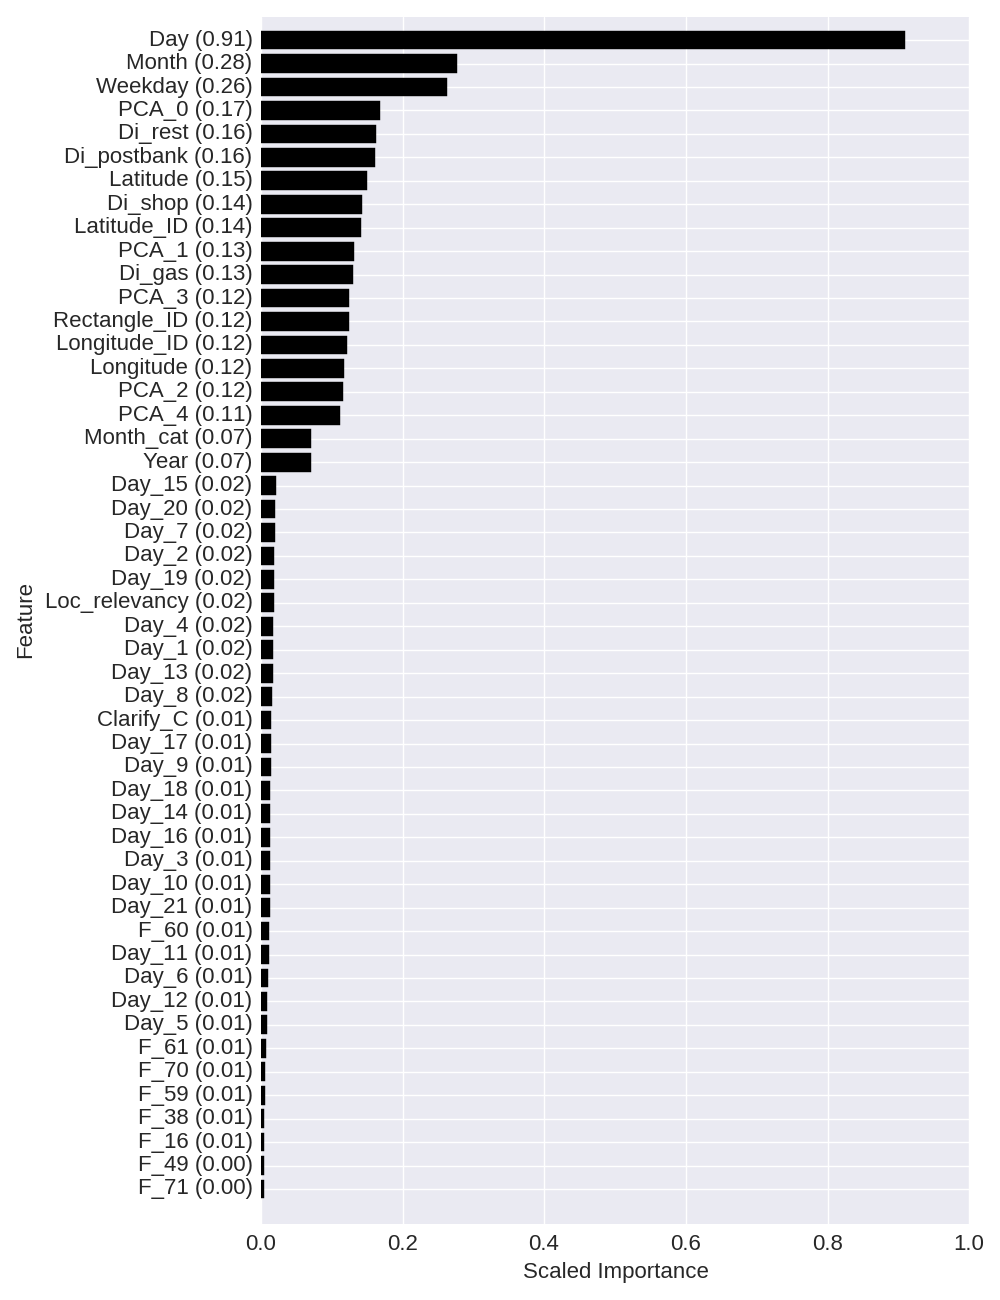
\includegraphics[scale=0.29]{feat_data_fi}\label{fig:roc_fe_fi}
    \caption{Feature importance of the best model trained on a combination time data and extracted features using \gls{cnn} and \gls{rnn} -- the first 50 features only.}
\end{figure}

In the figure~\ref{fig:roc_fe_best} the \gls{roc} analysis shows, that these features improve the prediction. The achieved \gls{auc} (0.731) is the highest from all tested models. 

\begin{figure}[ht]\centering
    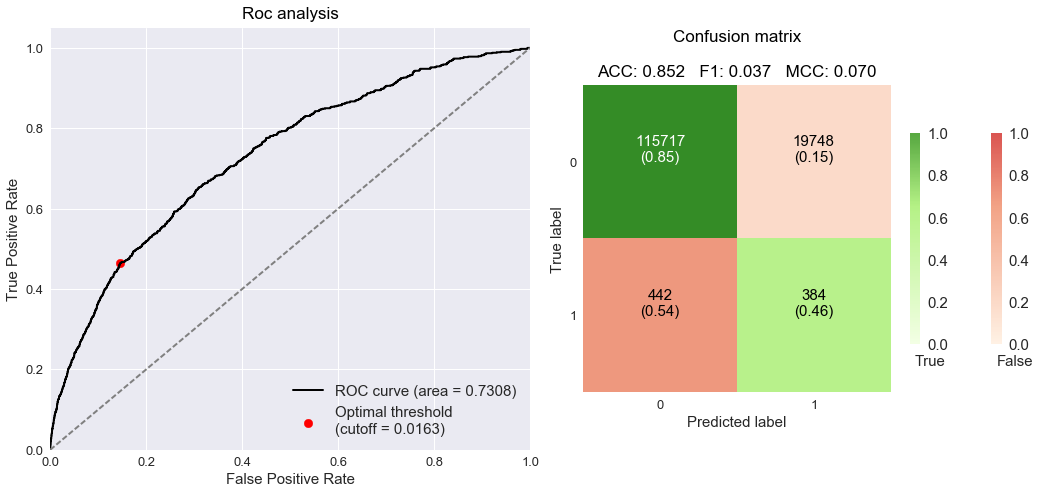
\includegraphics[scale=0.32]{roc_feat_data}\label{fig:roc_fe_best}
    \caption{Complete \gls{roc} analysis of the model trained on a combination time and extracted features using \gls{cnn} and \gls{rnn}.}
\end{figure}

Although the new features are not the best ranked in feature importance analysis (see figure~\ref{fig:roc_fe_fi}), they improved the prediction. The most important new extracted features is F\_60 which is preprocessed neighbour information from the previous day of the occurred crime. Otherwise, the other features are similar ranked as with model trained with the combination of the time and neighbour data.

This experiment shows that the combination of \gls{rnn} and \gls{cnn} to extract new features can improve prediction. The disadvantage this extraction approach is, that for generating new features, the new model has to be trained. When new data are stored, the best features can be obtained, if the old model is retrained with new data. It could be expensive to do this upgrade, for example, every day. 

\section{Analysis summary}

In this section, the result of all parts of the process and examined experiments are presented, which defined objectives were satisfied, and where some limits occurred.

During data preparation, the real crime data from the database of \gls{pcr} were using data mining techniques the data processed and transformed into the useful format for predictive analysis. The main emphasis was placed to get information from short-term history and near neighbourhood of occurred crimes to predict another risk areas in short-term future. Using feature selection methods, the quality of all features was estimated. As the most important were identified original data from the database of \gls{pcr} (such as date data and distances from nearest points of interest), but also new extracted features (such as components from \gls{pca} analysis and the information about crime activity the day before in the near neighbourhood). The data were modified for binary classification and split into training, validation and test datasets. 

In experimental section, it was proven that extracted features have the significant impact on prediction. The experiments were separated into four main part, where the effect of various features was measured -- first only on time data, then on neighbour, also on the combination of both and finally on data selected using feature selection approach. The experiments showed that more information is better than less. However, with correct feature selection, the result can be very similar as the best result with all data. 

The five main algorithms for predictive analysis were selected -- \gls{drf}, \gls{gbm}, \gls{dl}, \gls{cnn}, \gls{rnn}. The analysis exposed that the best performed are \gls{drf}s for this defined problem. They were the best with all type of data. Close to \gls{drf} were also \gls{gbm}. The \gls{dl}, \gls{cnn} and \gls{rnn} performed distinctly worse. For example, in most of cases the default setting of \gls{drf} model was still better than the best setting of \gls{dl}. However, it can be caused small number of experiments, especially with \gls{cnn} ans \gls{rnn} setting.

Using of the best performed models, the percentage of the correctly predicted crimes against false predicted crimes (\gls{tpr}) was approximately about 35 \% (see the table~\ref{tab:all_data_summary}, column \gls{tpr}). It is mainly due to selected threshold metrics (\gls{mcc}), which keep \gls{tpr} rather lower to avoid large increase of \gls{fpr} (with unbalanced data). The best models are significantly better than base models in comparison to \gls{f1} and \gls{mcc}, however, the result are very low, and there is still space for improvement (for example the better choice of hyperparameters or structure of models). 

The feature importance is the accessory output of models based on trees. Given well-performed \gls{drf} algorithm, the most important features can be evaluated from the best model of each type of data. On the top of feature ranking, the date information was in most of the cases (Day, Weekday, Week or Month). As crucial for division into classes were the distance from points of interest (Di\_postbank, Di\_rest, Di\_shop). From extracted features were the most important components from \gls{pca} (PCA\_0, PCA\_1, PCA\_2, PCA\_3, PCA\_4) and near neighbours in near history (Neigh\_60, Neigh\_61, Day\_7, Day\_15, etc.), how feature selection expected correctly. 

\gls{cnn} and \gls{rnn} were not performed well independently. In combination of both, the performance increased and was similar to \gls{dl} algorithm, however, it was not enough to \gls{drf}. Rather than for prediction, they were used for feature extraction and they improved the current best \gls{drf} model result \gls{auc} from 0.716 to 0.731 (see the table~\ref{tab:all_data_summary}, column \gls{auc}, model name DRF\_F\_B).

\begin{table}[H]\centering
\begin{scriptsize}
    \caption{Summary of best models of each algorithm trained on a all types of data -- results from confusion matrix and selected metrics.}\label{tab:all_data_summary}
    \begin{tabular}{|l|c|c|c|c|c|c|c|c|c|}\hline
        Model & Data & \gls{fnr} & \gls{tpr} & \gls{tnr} & \gls{fpr} & \gls{auc} & \gls{acc} & \gls{f1} & \gls{mcc} \tabularnewline \hline \hline
        DRF\_F\_B & 5 & 0.854 & 0.465 & 0.146 & 0.535 & 0.731 & 0.852 & 0.037 & 0.070 \tabularnewline  \hline
        DRF\_6\_5 & 3 & 0.935 & 0.267 & 0.065 & 0.733 & 0.716 & 0.931 & 0.047 & 0.065 \tabularnewline \hline
        DRF\_5\_3 & 4 & 0.921 & 0.294 & 0.079 & 0.706 & 0.715 & 0.917 & 0.043 & 0.063 \tabularnewline \hline
        DRF\_6\_5 & 2 & 0.940 & 0.259 & 0.060 & 0.741 & 0.716 & 0.931 & 0.047 & 0.065 \tabularnewline \hline
        DRF\_6\_3 & 1 & 0.842 & 0.422 & 0.157 & 0.578 & 0.701 & 0.840 & 0.033 & 0.058 \tabularnewline \hline
    \end{tabular}
\end{scriptsize}
\end{table}

The results from all performed models are in the appendix~\ref{appendix:result}. The 93 of models were evaluated so that the result table is large and have to be separated into three parts. The evaluated metrics have to be also separated into three tables due to the maximal size of the table. So that, the results of models are into nine tables, sorted first by \gls{auc}, secondly by \gls{mcc} and finally by \gls{tp}. 

Based on this analysis the answer to the question, if it is possible to use mainly historical non-personal data from the database of the \gls{pcr} for short-term prediction based on supervised learning algorithms, is yes, however with these conditions:

\begin{itemize}
    \item Data has to be quality and has to reflected the crime situation as much as possible, especially the more occurring crime, the better.
    \item Data has to be properly preprocessed and transformed into the suitable format for prediction.
    \item The more additional data (about an environment, the current situation in the areas, socio-geographical situation, etc.) the better.
    \item The problem has to be clearly defined because mainly based on this; the success can be evaluated.
    \item The accurate predictive methods and setting of hyperparameters has to be found and correctly implemented.
    \item Can not be assumed, that the accuracy of prediction will be perfect. The criminality is (fortunately) relatively small in the Czech Republic (in compare to how large is, for example, the Prague city and which places are every day in risk) so that the data are naturally extremely sparse and worse predictable.
    \item The evaluation, if the predictions are right in the real situation, is problematic. For example, the avoiding the crime is difficult measured immediately, and the increasing or decreasing tendency can be measured after some period. Or the criminality will just move to another place. 
\end{itemize}

It should be also considered, even the result preprocessed data was large, the explored area was in fact very small and reflected only specific part of Prague city. Also only one frequent type of crime was examined. The further research could be focused on verify the results of this process with more types of crime and compare the results. 

%%%%%%%%%%%%%%%%%%%%%%%%%%%%%%%%%%%%%%%%%%%%%%%%%%%%%%% CHAPTER %%%%%%%%%%%%%%%%%%%%%%%%%%%%%%%%%%%%%%%%%%%%%%%%%%%%%%%

\chapter{Recommendation for the Police of the Czech Republic}\label{sec:recommendation}

The following recommendations are inspired by the whole process from understanding problematics of the criminality prediction, problem definition, data processing to predictive methods description and final analysis completion. The recommendations are divided into three main parts - about data, about analysis, about implementation.  

\section{About data}

Data are the basis of all analysis. It is crucial to maintaining the criminal data actual and quality. Data should be in the structured format and be available for analysts (or possible developers) instantly.

The crucial for the quality of data is the systems which police officers use to collect data. For example, the wrong system which allows users to insert values, which are inconsistent, incorrect or in an inappropriate format. Also, the data are prone to contain incorrect values if they come from many sources. 

Analysis of feature importance shows that data from near surrounding of crime has a positive impact on prediction. The \gls{pcr} develops own \gls{gis} system, which can be the great source of important data for prediction. For further research, I recommended extracting as many information as possible from this useful tool and other available sources (for example more points of interest, socio-geographic data, weather data, economic data, police patrol movement of people, etc.).


\newpage
\section{About analysis}

The analysis shows that for prediction is essential to properly define problem and based on this choose the right model or set of procedures. In this thesis, the \gls{drf} were best accurate models. However, it does not mean that \gls{drf} solve every defined problem from now. The good practice is to try more models during analysis and then select the best. 

The amount of data is also crucial for correct result interpretation. The more occurring crime will be probably better predicted using general machine learning algorithms. For prediction less occurring crime, more particular methods and practices of investigation have to be used. 

The experiments show, that there are many other possibilities to defined problem and to reach the different results. The creativity is also important during predictive analysis. The plenty of transformation of data can significantly improve prediction. For example the \gls{cnn} has a problem with sparse data and does not perform well. To improve the performance, input images can condensate information from a defined sequence of days (for example hot-spots from the previous week). The longer time sequence can, for example, improve predictions of \gls{rnn}.

In this thesis, the only small area of Prague city was studied. The next step of analysis should be to verify this process also for other types of crime. Firstly, I prepared more types of crime, however, to process more types of crime was out of the scope of this thesis. 

\section{About implementation}

The proper analysis consumes hundreds of hours of experienced data analysis, is not cheap and it is never ending process. To solve this problem, several approaches exist. First to buy proprietary software, to learn with them and pay for support. The another possibility is to developed own predictive system and still improve it. 
In the case of own implementation, it is important to select an experienced company or to employ competent software engineers, which they have skill with implementing predictive systems. 

It can not be forgotten that every system has to be maintained and especially the prediction system require updates (for example retrained model with new data) more often than others systems. For processing big amount of data, the big data storage and huge computing power are necessary.

The system itself does not reduce criminality even if it is accurate and efficient. The introduction of a new system into practice also brings inconveniences and requires cooperation at all levels of the police structure. 

\begin{conclusion}
    
    This thesis was focused on criminality prediction with emphasis on testing this approach with the real-world crime data. In the first part of the thesis, the theoretical background was introduced, and the concept of predictive analysis was described. In the practical part using the \gls{crisp} process the crime data obtained from the \gls{pcr} were analysed, and new information was gained. Finally, the recommendation for \gls{pcr} was put together based on gained experience. 
    
    The main goal of this research was to understand the problematics of criminality prediction and try how accurate are the modern methods of supervised learning with real crime data from the Czech Republic, especially from the Prague city. After problem definition and the data preprocessing the amount of the data rapidly increase but the resulting data are extremely sparse. The only smaller area had to be selected, and the whole analysis was related to this section and one selected often occurring type of crime. 
    
    Despite the limitations, the result of research can be used to understand criminality prediction better. The predictive models based on \gls{drf}, \gls{gbm}, \gls{dl}, \gls{cnn} and \gls{rnn} algorithms were trained and tested using selected crime data. The experiments show, that the best accurate are models based on \gls{drf} algorithm. The average percentage of correctly predicted crimes using best models was approximately 35 \%, but on optimise false crime prediction too. 
    
    Then the importance of features was inspected. Based on the result from the best accurate models, the most important for tree building are information about the date the observed area, the distance of the nearest point of interest (bank, post office, restaurant, gas station, shop). But also new extracted features improved prediction. The research also mentioned that there plenty of the other possibilities how to interpret data and improve the predictions.  
    
    Finally, the recommendations for \gls{pcr} were summarised. The most important are to realise, that a new predictive system itself does not reduce criminality and it does not take the full control over the decision-making of the police officers. However, it could be a useful tool for effective work within the \gls{pcr}. 
    
    As mentioned before, the only relatively small area of Prague city was analysed, and only one type of crime was selected. The next step of further research could be to verify the whole process with the other types of crime and to compare the results. The different areas of the Czech Republic could be selected and different models evaluated using them. Other approaches could be tried, for example, to combine more different models or for every unit on the map fit the different model.
    
    I chose this topic for purpose of working with real data and solving of the interesting problem. The main personal goal was to make it useful. The whole thesis includes the scripts of analysis will be given to free download and reused. Unfortunately, the source data can not be published because were borrowed only for research purposes.
	
\end{conclusion}

\bibliographystyle{iso690.bst}
\bibliography{ref}

\setsecnumdepth{all}
\appendix

\chapter{Experiment results}\label{appendix:result}

\begin{table}[H]\centering
\begin{small}
    \caption{Summary of best models of each algorithm trained on a all types of data -- part 1.1}\label{tab:all_data_summary_1_1}
    \begin{tabular}{|l|l|c|c|c|c|}\hline
        Data & Model & \gls{tn} & \gls{fn} & \gls{tp} & \gls{fp} \tabularnewline \hline \hline
feat\_data & DRF\_F\_B & 115\,717 & 19\,748 & 384 & 442 \tabularnewline  \hline 
all\_data & DRF\_6\_5 & 161\,733 & 11\,213 & 298 & 819 \tabularnewline  \hline 
fs\_data & DRF\_5\_3 & 159\,244 & 13\,702 & 328 & 789 \tabularnewline  \hline 
all\_data & DRF\_7\_4 & 168\,749 & 4\,197 & 174 & 943 \tabularnewline  \hline 
all\_data & DRF\_6\_3 & 155\,551 & 17\,395 & 385 & 732 \tabularnewline  \hline 
fs\_data & DRF\_5\_3 & 149\,637 & 23\,309 & 436 & 681 \tabularnewline  \hline 
fs\_data & DRF\_6\_3 & 159\,895 & 13\,051 & 309 & 808 \tabularnewline  \hline 
neigh\_data & DRF\_7\_4 & 162\,543 & 10\,403 & 289 & 828 \tabularnewline  \hline 
all\_data & DRF\_default & 149\,754 & 23\,192 & 421 & 696 \tabularnewline  \hline 
neigh\_data & DRF\_6\_5 & 161\,825 & 11\,121 & 293 & 824 \tabularnewline  \hline 
neigh\_data & DRF\_4\_3 & 160\,380 & 12\,566 & 316 & 801 \tabularnewline  \hline 
fs\_data & DRF\_default & 113\,114 & 59\,832 & 737 & 380 \tabularnewline  \hline 
tm\_data & DRF\_6\_3 & 145\,713 & 27\,233 & 471 & 646 \tabularnewline  \hline 
all\_data & GBM\_6\_1 & 166\,687 & 6\,259 & 213 & 904 \tabularnewline  \hline 
tm\_data & DRF\_7\_4 & 159\,781 & 13\,165 & 321 & 796 \tabularnewline  \hline 
all\_data & GBM\_5\_1 & 166\,960 & 5\,986 & 204 & 913 \tabularnewline  \hline 
tm\_data & GBM\_6\_1 & 163\,082 & 9\,864 & 252 & 865 \tabularnewline  \hline 
fs\_data & GBM\_4\_2 & 169\,625 & 3\,321 & 127 & 990 \tabularnewline  \hline 
fs\_data & GBM\_3\_2 & 169\,625 & 3\,321 & 127 & 990 \tabularnewline  \hline 
tm\_data & GBM\_5\_1 & 169\,856 & 3\,090 & 127 & 990 \tabularnewline  \hline 
fs\_data & GBM\_2\_2 & 169\,537 & 3\,409 & 129 & 988 \tabularnewline  \hline 
all\_data & GBM\_default & 168\,018 & 4\,928 & 173 & 944 \tabularnewline  \hline 
all\_data & GBM\_4\_1 & 166\,925 & 6\,021 & 198 & 919 \tabularnewline  \hline 
tm\_data & GBM\_default & 170\,380 & 2\,566 & 116 & 1\,001 \tabularnewline  \hline 
tm\_data & GBM\_4\_1 & 169\,969 & 2\,977 & 127 & 990 \tabularnewline  \hline 
neigh\_data & GBM\_default & 168\,222 & 4\,724 & 170 & 947 \tabularnewline  \hline 
tm\_data & DRF\_6\_5 & 153\,288 & 19\,658 & 392 & 725 \tabularnewline  \hline 
fs\_data & GBM\_default & 169\,215 & 3\,731 & 149 & 968 \tabularnewline  \hline 
neigh\_data & GBM\_6\_1 & 163\,479 & 9\,467 & 242 & 875 \tabularnewline  \hline 
neigh\_data & GBM\_4\_1 & 163\,479 & 9\,467 & 242 & 875 \tabularnewline  \hline 
neigh\_data & GBM\_5\_1 & 163\,479 & 9\,467 & 242 & 875 \tabularnewline  \hline 
    \end{tabular}
\end{small}
\end{table}


\begin{table}[H]\centering
\begin{small}
    \caption{Summary of best models of each algorithm trained on a all types of data -- part 1.2}\label{tab:all_data_summary_1_2}
    \begin{tabular}{|l|l|c|c|c|c|}\hline
Data & Model & \gls{tn} & \gls{fn} & \gls{tp} & \gls{fp} \tabularnewline \hline \hline
neigh\_data & DRF\_default & 158\,503 & 14\,443 & 310 & 807 \tabularnewline  \hline 
tm\_data & DRF\_default & 149\,514 & 23\,432 & 399 & 718 \tabularnewline  \hline 
tm\_data & DEL\_1\_3 & 168\,734 & 4\,212 & 124 & 993 \tabularnewline  \hline 
fs\_data & DEL\_5\_3 & 145\,485 & 27\,461 & 412 & 705 \tabularnewline  \hline 
fs\_data & DEL\_4\_3 & 169\,004 & 3\,942 & 129 & 988 \tabularnewline  \hline 
all\_data & DEL\_5\_3 & 158\,443 & 14\,503 & 266 & 851 \tabularnewline  \hline 
all\_data & CRNN\_2\_8\_1\_100 & 130\,371 & 59\,189 & 699 & 547 \tabularnewline  \hline 
fs\_data & DEL\_2\_1 & 161\,555 & 11\,391 & 227 & 890 \tabularnewline  \hline 
all\_data & CRNN\_2\_8\_1\_100 & 140\,804 & 48\,756 & 620 & 626 \tabularnewline  \hline 
all\_data & DEL\_5\_2 & 168\,251 & 4\,695 & 145 & 972 \tabularnewline  \hline 
all\_data & CRNN\_2\_16\_1\_100 & 140\,759 & 48\,801 & 622 & 624 \tabularnewline  \hline 
all\_data & CRNN\_2\_8\_1\_100 & 121\,715 & 67\,845 & 768 & 478 \tabularnewline  \hline 
tm\_data & DEL\_5\_2 & 148\,092 & 24\,854 & 365 & 752 \tabularnewline  \hline 
all\_data & DEL\_4\_1 & 163\,925 & 9\,021 & 204 & 913 \tabularnewline  \hline 
all\_data & CRNN\_2\_32\_1\_100 & 138\,990 & 50\,570 & 616 & 630 \tabularnewline  \hline 
tm\_data & DEL\_3\_3 & 166\,799 & 6\,147 & 168 & 949 \tabularnewline  \hline 
all\_data & CRNN\_2\_16\_1\_100 & 142\,484 & 47\,076 & 583 & 663 \tabularnewline  \hline 
all\_data & CRNN\_8\_4\_1\_100 & 146\,705 & 42\,855 & 553 & 693 \tabularnewline  \hline 
all\_data & CRNN\_2\_32\_1\_100 & 116\,912 & 72\,648 & 787 & 459 \tabularnewline  \hline 
all\_data & CRNN\_1\_32\_1\_50 & 120\,981 & 68\,579 & 752 & 494 \tabularnewline  \hline 
all\_data & CRNN\_4\_32\_1\_50 & 112\,618 & 76\,942 & 807 & 439 \tabularnewline  \hline 
all\_data & CRNN\_2\_8\_1\_100 & 165\,392 & 24\,168 & 368 & 878 \tabularnewline  \hline 
neigh\_data & DEL\_default & 114\,700 & 58\,246 & 650 & 467 \tabularnewline  \hline 
neigh\_data & DEL\_5\_3 & 117\,836 & 55\,110 & 625 & 492 \tabularnewline  \hline 
neigh\_data & DEL\_1\_2 & 109\,220 & 63\,726 & 685 & 432 \tabularnewline  \hline 
all\_data & CRNN\_2\_32\_1\_50 & 115\,246 & 74\,314 & 773 & 473 \tabularnewline  \hline 
neigh\_data & DEL\_5\_2 & 94\,404 & 78\,542 & 761 & 356 \tabularnewline  \hline 
all\_data & CRNN\_4\_16\_1\_100 & 132\,023 & 57\,537 & 624 & 622 \tabularnewline  \hline 
all\_data & CRNN\_4\_32\_1\_100 & 158\,142 & 31\,418 & 405 & 841 \tabularnewline  \hline 
tm\_data & DEL\_default & 165\,124 & 7\,822 & 145 & 972 \tabularnewline  \hline 
neigh\_data & CNN\_2\_64 & 142\,277 & 30\,669 & 341 & 776 \tabularnewline  \hline 
tm\_data & RNN\_2\_100 & 172\,419 & 526 & 47 & 1\,071 \tabularnewline  \hline 
    \end{tabular}
\end{small}
\end{table}

\begin{table}[H]\centering
\begin{small}
    \caption{Summary of best models of each algorithm trained on a all types of data -- part 1.3}\label{tab:all_data_summary_1_3}
    \begin{tabular}{|l|l|c|c|c|c|}\hline
Data & Model & \gls{tn} & \gls{fn} & \gls{tp} & \gls{fp} \tabularnewline \hline \hline
tm\_data & RNN\_2\_100 & 172\,778 & 167 & 29 & 1\,089 \tabularnewline  \hline 
neigh\_data & CNN\_2\_256 & 147\,796 & 25\,150 & 298 & 819 \tabularnewline  \hline 
neigh\_data & CNN\_4\_32 & 150\,939 & 22\,007 & 269 & 848 \tabularnewline  \hline 
neigh\_data & CNN\_2\_16 & 139\,287 & 33\,659 & 369 & 748 \tabularnewline  \hline 
neigh\_data & CNN\_2\_8 & 141\,658 & 31\,288 & 349 & 768 \tabularnewline  \hline 
neigh\_data & CNN\_2\_128 & 140\,086 & 32\,860 & 363 & 754 \tabularnewline  \hline 
fs\_data & DEL\_default & 57\,900 & 115\,046 & 918 & 199 \tabularnewline  \hline 
all\_data & DEL\_default & 65\,966 & 106\,980 & 843 & 274 \tabularnewline  \hline 
neigh\_data & CNN\_2\_32 & 140\,664 & 32\,282 & 357 & 760 \tabularnewline  \hline 
neigh\_data & CNN\_4\_32 & 154\,526 & 18\,420 & 235 & 882 \tabularnewline  \hline 
neigh\_data & CNN\_4\_16 & 149\,707 & 23\,239 & 276 & 841 \tabularnewline  \hline 
neigh\_data & CNN\_8\_16 & 158\,332 & 14\,614 & 203 & 914 \tabularnewline  \hline 
neigh\_data & CNN\_8\_16 & 158\,557 & 14\,389 & 202 & 915 \tabularnewline  \hline 
neigh\_data & CNN\_4\_8 & 138\,664 & 34\,282 & 375 & 742 \tabularnewline  \hline 
neigh\_data & CNN\_4\_32 & 153\,329 & 19\,617 & 249 & 868 \tabularnewline  \hline 
tm\_data & RNN\_2\_32 & 156\,747 & 16\,198 & 280 & 838 \tabularnewline  \hline 
tm\_data & RNN\_1\_254 & 156\,969 & 15\,976 & 272 & 846 \tabularnewline  \hline 
tm\_data & RNN\_4\_32 & 157\,779 & 15\,166 & 252 & 866 \tabularnewline  \hline 
tm\_data & RNN\_1\_121 & 163\,866 & 9\,079 & 181 & 937 \tabularnewline  \hline 
tm\_data & RNN\_1\_50 & 162\,955 & 9\,990 & 190 & 928 \tabularnewline  \hline 
tm\_data & RNN\_1\_100 & 163\,900 & 9\,045 & 179 & 939 \tabularnewline  \hline 
all\_data & CRNN\_2\_32\_2\_21 & 162\,574 & 26\,986 & 228 & 1\,018 \tabularnewline  \hline 
all\_data & CRNN\_2\_32\_1\_100 & 147\,053 & 42\,507 & 322 & 924 \tabularnewline  \hline 
all\_data & CRNN\_2\_32\_2\_100 & 7\,068 & 182\,492 & 1\,221 & 25 \tabularnewline  \hline 
neigh\_data & CNN\_8\_8 & 0 & 172\,946 & 1\,117 & 0 \tabularnewline  \hline 
all\_data & CRNN\_2\_32\_4\_21 & 180\,548 & 9\,012 & 74 & 1\,172 \tabularnewline  \hline 
tm\_data & RNN\_8\_21 & 166\,794 & 6\,151 & 124 & 994 \tabularnewline  \hline 
tm\_data & RNN\_4\_21 & 167\,798 & 5\,147 & 76 & 1\,042 \tabularnewline  \hline 
tm\_data & RNN\_8\_8 & 1 & 172\,944 & 1\,118 & 0 \tabularnewline  \hline 
tm\_data & RNN\_2\_32 & 1 & 172\,944 & 1\,118 & 0 \tabularnewline  \hline 
    \end{tabular}
\end{small}
\end{table}


\begin{table}[H]\centering
\begin{small}
    \caption{Summary of best models of each algorithm trained on a all types of data -- part 2.1}\label{tab:all_data_summary_2_1}
    \begin{tabular}{|l|l|c|c|c|c|c|}\hline
Data & Model & \gls{auc} & \gls{acc} & \gls{f1} & \gls{mcc} & threshold \tabularnewline \hline \hline
feat\_data & DRF\_F\_B & 0.731 & 0.852 & 0.037 & 0.070 & 0.016 \tabularnewline  \hline 
all\_data & DRF\_6\_5 & 0.716 & 0.931 & 0.047 & 0.065 & 0.026 \tabularnewline  \hline 
fs\_data & DRF\_5\_3 & 0.715 & 0.917 & 0.043 & 0.063 & 0.026 \tabularnewline  \hline 
all\_data & DRF\_7\_4 & 0.715 & 0.970 & 0.063 & 0.067 & 0.037 \tabularnewline  \hline 
all\_data & DRF\_6\_3 & 0.712 & 0.896 & 0.041 & 0.064 & 0.021 \tabularnewline  \hline 
fs\_data & DRF\_5\_3 & 0.711 & 0.862 & 0.035 & 0.059 & 0.020 \tabularnewline  \hline 
fs\_data & DRF\_6\_3 & 0.711 & 0.920 & 0.043 & 0.060 & 0.025 \tabularnewline  \hline 
neigh\_data & DRF\_7\_4 & 0.711 & 0.935 & 0.049 & 0.066 & 0.025 \tabularnewline  \hline 
all\_data & DRF\_default & 0.705 & 0.863 & 0.034 & 0.057 & 0.017 \tabularnewline  \hline 
neigh\_data & DRF\_6\_5 & 0.704 & 0.931 & 0.047 & 0.064 & 0.025 \tabularnewline  \hline 
neigh\_data & DRF\_4\_3 & 0.703 & 0.923 & 0.045 & 0.064 & 0.023 \tabularnewline  \hline 
fs\_data & DRF\_default & 0.702 & 0.654 & 0.024 & 0.053 & 0.012 \tabularnewline  \hline 
tm\_data & DRF\_6\_3 & 0.701 & 0.840 & 0.033 & 0.058 & 0.017 \tabularnewline  \hline 
all\_data & GBM\_6\_1 & 0.701 & 0.959 & 0.056 & 0.065 & 0.024 \tabularnewline  \hline 
tm\_data & DRF\_7\_4 & 0.701 & 0.920 & 0.044 & 0.063 & 0.024 \tabularnewline  \hline 
all\_data & GBM\_5\_1 & 0.701 & 0.960 & 0.056 & 0.064 & 0.024 \tabularnewline  \hline 
tm\_data & GBM\_6\_1 & 0.700 & 0.938 & 0.045 & 0.058 & 0.021 \tabularnewline  \hline 
fs\_data & GBM\_4\_2 & 0.699 & 0.975 & 0.056 & 0.054 & 0.036 \tabularnewline  \hline 
fs\_data & GBM\_3\_2 & 0.699 & 0.975 & 0.056 & 0.054 & 0.036 \tabularnewline  \hline 
tm\_data & GBM\_5\_1 & 0.699 & 0.977 & 0.059 & 0.057 & 0.030 \tabularnewline  \hline 
fs\_data & GBM\_2\_2 & 0.699 & 0.975 & 0.055 & 0.054 & 0.035 \tabularnewline  \hline 
all\_data & GBM\_default & 0.699 & 0.966 & 0.056 & 0.060 & 0.025 \tabularnewline  \hline 
all\_data & GBM\_4\_1 & 0.698 & 0.960 & 0.054 & 0.061 & 0.023 \tabularnewline  \hline 
tm\_data & GBM\_default & 0.698 & 0.980 & 0.061 & 0.058 & 0.030 \tabularnewline  \hline 
tm\_data & GBM\_4\_1 & 0.698 & 0.977 & 0.060 & 0.058 & 0.029 \tabularnewline  \hline 
neigh\_data & GBM\_default & 0.697 & 0.967 & 0.057 & 0.060 & 0.026 \tabularnewline  \hline 
tm\_data & DRF\_6\_5 & 0.697 & 0.883 & 0.037 & 0.059 & 0.021 \tabularnewline  \hline 
fs\_data & GBM\_default & 0.697 & 0.973 & 0.060 & 0.060 & 0.027 \tabularnewline  \hline 
neigh\_data & GBM\_6\_1 & 0.696 & 0.941 & 0.045 & 0.056 & 0.022 \tabularnewline  \hline 
neigh\_data & GBM\_4\_1 & 0.696 & 0.941 & 0.045 & 0.056 & 0.022 \tabularnewline  \hline 
neigh\_data & GBM\_5\_1 & 0.696 & 0.941 & 0.045 & 0.056 & 0.022 \tabularnewline  \hline 
    \end{tabular}
\end{small}
\end{table}

\begin{table}[H]\centering
\begin{small}
    \caption{Summary of best models of each algorithm trained on a all types of data -- part 2.2}\label{tab:all_data_summary_2_2}
    \begin{tabular}{|l|l|c|c|c|c|c|}\hline
    Data & Model & \gls{auc} & \gls{acc} & \gls{f1} & \gls{mcc} & threshold \tabularnewline \hline \hline
neigh\_data & DRF\_default & 0.696 & 0.912 & 0.039 & 0.056 & 0.021 \tabularnewline  \hline 
tm\_data & DRF\_default & 0.688 & 0.861 & 0.032 & 0.052 & 0.017 \tabularnewline  \hline 
tm\_data & DEL\_1\_3 & 0.679 & 0.970 & 0.045 & 0.044 & 0.022 \tabularnewline  \hline 
fs\_data & DEL\_5\_3 & 0.678 & 0.838 & 0.028 & 0.046 & 0.009 \tabularnewline  \hline 
fs\_data & DEL\_4\_3 & 0.674 & 0.972 & 0.050 & 0.049 & 0.027 \tabularnewline  \hline 
all\_data & DEL\_5\_3 & 0.672 & 0.912 & 0.033 & 0.044 & 0.014 \tabularnewline  \hline 
all\_data & CRNN\_2\_8\_1\_100 & 0.669 & 0.687 & 0.023 & 0.043 & 0.017 \tabularnewline  \hline 
fs\_data & DEL\_2\_1 & 0.669 & 0.929 & 0.036 & 0.044 & 0.006 \tabularnewline  \hline 
all\_data & CRNN\_2\_8\_1\_100 & 0.668 & 0.741 & 0.025 & 0.044 & 0.023 \tabularnewline  \hline 
all\_data & DEL\_5\_2 & 0.668 & 0.967 & 0.049 & 0.050 & 0.019 \tabularnewline  \hline 
all\_data & CRNN\_2\_16\_1\_100 & 0.667 & 0.741 & 0.025 & 0.044 & 0.021 \tabularnewline  \hline 
all\_data & CRNN\_2\_8\_1\_100 & 0.666 & 0.642 & 0.022 & 0.043 & 0.015 \tabularnewline  \hline 
tm\_data & DEL\_5\_2 & 0.665 & 0.853 & 0.028 & 0.042 & 0.017 \tabularnewline  \hline 
all\_data & DEL\_4\_1 & 0.663 & 0.943 & 0.039 & 0.047 & 0.011 \tabularnewline  \hline 
all\_data & CRNN\_2\_32\_1\_100 & 0.662 & 0.732 & 0.024 & 0.041 & 0.020 \tabularnewline  \hline 
tm\_data & DEL\_3\_3 & 0.661 & 0.959 & 0.045 & 0.049 & 0.020 \tabularnewline  \hline 
all\_data & CRNN\_2\_16\_1\_100 & 0.660 & 0.750 & 0.024 & 0.041 & 0.014 \tabularnewline  \hline 
all\_data & CRNN\_8\_4\_1\_100 & 0.660 & 0.772 & 0.025 & 0.042 & 0.016 \tabularnewline  \hline 
all\_data & CRNN\_2\_32\_1\_100 & 0.658 & 0.617 & 0.021 & 0.041 & 0.013 \tabularnewline  \hline 
all\_data & CRNN\_1\_32\_1\_50 & 0.656 & 0.638 & 0.021 & 0.040 & 0.014 \tabularnewline  \hline 
all\_data & CRNN\_4\_32\_1\_50 & 0.656 & 0.594 & 0.020 & 0.040 & 0.015 \tabularnewline  \hline 
all\_data & CRNN\_2\_8\_1\_100 & 0.656 & 0.869 & 0.029 & 0.040 & 0.026 \tabularnewline  \hline 
neigh\_data & DEL\_default & 0.650 & 0.663 & 0.022 & 0.041 & 0.010 \tabularnewline  \hline 
neigh\_data & DEL\_5\_3 & 0.649 & 0.681 & 0.022 & 0.041 & 0.004 \tabularnewline  \hline 
neigh\_data & DEL\_1\_2 & 0.648 & 0.631 & 0.021 & 0.040 & 0.007 \tabularnewline  \hline 
all\_data & CRNN\_2\_32\_1\_50 & 0.648 & 0.608 & 0.020 & 0.038 & 0.018 \tabularnewline  \hline 
neigh\_data & DEL\_5\_2 & 0.641 & 0.547 & 0.019 & 0.036 & 0.009 \tabularnewline  \hline 
all\_data & CRNN\_4\_16\_1\_100 & 0.636 & 0.695 & 0.021 & 0.035 & 0.012 \tabularnewline  \hline 
all\_data & CRNN\_4\_32\_1\_100 & 0.634 & 0.831 & 0.024 & 0.034 & 0.017 \tabularnewline  \hline 
tm\_data & DEL\_default & 0.623 & 0.949 & 0.032 & 0.032 & 0.022 \tabularnewline  \hline 
neigh\_data & CNN\_2\_64 & 0.590 & 0.819 & 0.021 & 0.027 & 0.010 \tabularnewline  \hline 
tm\_data & RNN\_2\_100 & 0.589 & 0.991 & 0.056 & 0.054 & 0.220 \tabularnewline  \hline 
    \end{tabular}
\end{small}
\end{table}

\begin{table}[H]\centering
\begin{small}
    \caption{Summary of best models of each algorithm trained on a all types of data -- part 2.3}\label{tab:all_data_summary_2_3}
    \begin{tabular}{|l|l|c|c|c|c|c|}\hline
        Data & Model & \gls{auc} & \gls{acc} & \gls{f1} & \gls{mcc} & threshold \tabularnewline \hline \hline
tm\_data & RNN\_2\_100 & 0.589 & 0.993 & 0.044 & 0.059 & 0.401 \tabularnewline  \hline 
neigh\_data & CNN\_2\_256 & 0.586 & 0.851 & 0.022 & 0.027 & 0.015 \tabularnewline  \hline 
neigh\_data & CNN\_4\_32 & 0.586 & 0.869 & 0.023 & 0.027 & 0.016 \tabularnewline  \hline 
neigh\_data & CNN\_2\_16 & 0.586 & 0.802 & 0.021 & 0.027 & 0.014 \tabularnewline  \hline 
neigh\_data & CNN\_2\_8 & 0.586 & 0.816 & 0.021 & 0.027 & 0.016 \tabularnewline  \hline 
neigh\_data & CNN\_2\_128 & 0.586 & 0.807 & 0.021 & 0.027 & 0.009 \tabularnewline  \hline 
fs\_data & DEL\_default & 0.585 & 0.338 & 0.016 & 0.027 & 0.006 \tabularnewline  \hline 
all\_data & DEL\_default & 0.585 & 0.384 & 0.015 & 0.022 & 0.008 \tabularnewline  \hline 
neigh\_data & CNN\_2\_32 & 0.584 & 0.810 & 0.021 & 0.027 & 0.010 \tabularnewline  \hline 
neigh\_data & CNN\_4\_32 & 0.582 & 0.889 & 0.024 & 0.027 & 0.011 \tabularnewline  \hline 
neigh\_data & CNN\_4\_16 & 0.581 & 0.862 & 0.022 & 0.026 & 0.012 \tabularnewline  \hline 
neigh\_data & CNN\_8\_16 & 0.578 & 0.911 & 0.025 & 0.028 & 0.016 \tabularnewline  \hline 
neigh\_data & CNN\_8\_16 & 0.577 & 0.912 & 0.026 & 0.028 & 0.013 \tabularnewline  \hline 
neigh\_data & CNN\_4\_8 & 0.577 & 0.799 & 0.021 & 0.027 & 0.011 \tabularnewline  \hline 
neigh\_data & CNN\_4\_32 & 0.575 & 0.882 & 0.024 & 0.028 & 0.016 \tabularnewline  \hline 
tm\_data & RNN\_2\_32 & 0.571 & 0.902 & 0.032 & 0.043 & 0.011 \tabularnewline  \hline 
tm\_data & RNN\_1\_254 & 0.567 & 0.903 & 0.031 & 0.041 & 0.010 \tabularnewline  \hline 
tm\_data & RNN\_4\_32 & 0.553 & 0.908 & 0.030 & 0.039 & 0.011 \tabularnewline  \hline 
tm\_data & RNN\_1\_121 & 0.544 & 0.942 & 0.035 & 0.039 & 0.012 \tabularnewline  \hline 
tm\_data & RNN\_1\_50 & 0.538 & 0.937 & 0.034 & 0.038 & 0.011 \tabularnewline  \hline 
tm\_data & RNN\_1\_100 & 0.535 & 0.943 & 0.035 & 0.038 & 0.011 \tabularnewline  \hline 
all\_data & CRNN\_2\_32\_2\_21 & 0.521 & 0.853 & 0.016 & 0.009 & 0.011 \tabularnewline  \hline 
all\_data & CRNN\_2\_32\_1\_100 & 0.517 & 0.772 & 0.015 & 0.007 & 0.010 \tabularnewline  \hline 
all\_data & CRNN\_2\_32\_2\_100 & 0.504 & 0.043 & 0.013 & 0.007 & 0.008 \tabularnewline  \hline 
neigh\_data & CNN\_8\_8 & 0.500 & 0.006 & 0.013 & 0.000 & 0.012 \tabularnewline  \hline 
all\_data & CRNN\_2\_32\_4\_21 & 0.497 & 0.947 & 0.014 & 0.004 & 0.011 \tabularnewline  \hline 
tm\_data & RNN\_8\_21 & 0.495 & 0.959 & 0.034 & 0.032 & 0.011 \tabularnewline  \hline 
tm\_data & RNN\_4\_21 & 0.451 & 0.964 & 0.024 & 0.018 & 0.013 \tabularnewline  \hline 
tm\_data & RNN\_8\_8 & 0.430 & 0.006 & 0.013 & 0.000 & 0.012 \tabularnewline  \hline 
tm\_data & RNN\_2\_32 & 0.413 & 0.006 & 0.013 & 0.000 & 0.011 \tabularnewline  \hline 
    \end{tabular}
\end{small}
\end{table}


\begin{table}[H]\centering
\begin{small}
    \caption{Summary of best models of each algorithm trained on a all types of data -- part 3.1}\label{tab:all_data_summary_3_1}
    \begin{tabular}{|l|l|c|c|c|c|}\hline
Data & Model & \gls{tnr} & \gls{tpr} & \gls{fnr} & \gls{fpr} \tabularnewline \hline \hline
feat\_data & DRF\_F\_B & 0.854 & 0.465 & 0.146 & 0.535 \tabularnewline  \hline 
all\_data & DRF\_6\_5 & 0.935 & 0.267 & 0.065 & 0.733 \tabularnewline  \hline 
fs\_data & DRF\_5\_3 & 0.921 & 0.294 & 0.079 & 0.706 \tabularnewline  \hline 
all\_data & DRF\_7\_4 & 0.976 & 0.156 & 0.024 & 0.844 \tabularnewline  \hline 
all\_data & DRF\_6\_3 & 0.899 & 0.345 & 0.101 & 0.655 \tabularnewline  \hline 
fs\_data & DRF\_5\_3 & 0.865 & 0.390 & 0.135 & 0.610 \tabularnewline  \hline 
fs\_data & DRF\_6\_3 & 0.925 & 0.277 & 0.075 & 0.723 \tabularnewline  \hline 
neigh\_data & DRF\_7\_4 & 0.940 & 0.259 & 0.060 & 0.741 \tabularnewline  \hline 
all\_data & DRF\_default & 0.866 & 0.377 & 0.134 & 0.623 \tabularnewline  \hline 
neigh\_data & DRF\_6\_5 & 0.936 & 0.262 & 0.064 & 0.738 \tabularnewline  \hline 
neigh\_data & DRF\_4\_3 & 0.927 & 0.283 & 0.073 & 0.717 \tabularnewline  \hline 
fs\_data & DRF\_default & 0.654 & 0.660 & 0.346 & 0.340 \tabularnewline  \hline 
tm\_data & DRF\_6\_3 & 0.843 & 0.422 & 0.157 & 0.578 \tabularnewline  \hline 
all\_data & GBM\_6\_1 & 0.964 & 0.191 & 0.036 & 0.809 \tabularnewline  \hline 
tm\_data & DRF\_7\_4 & 0.924 & 0.287 & 0.076 & 0.713 \tabularnewline  \hline 
all\_data & GBM\_5\_1 & 0.965 & 0.183 & 0.035 & 0.817 \tabularnewline  \hline 
tm\_data & GBM\_6\_1 & 0.943 & 0.226 & 0.057 & 0.774 \tabularnewline  \hline 
fs\_data & GBM\_4\_2 & 0.981 & 0.114 & 0.019 & 0.886 \tabularnewline  \hline 
fs\_data & GBM\_3\_2 & 0.981 & 0.114 & 0.019 & 0.886 \tabularnewline  \hline 
tm\_data & GBM\_5\_1 & 0.982 & 0.114 & 0.018 & 0.886 \tabularnewline  \hline 
fs\_data & GBM\_2\_2 & 0.980 & 0.115 & 0.020 & 0.885 \tabularnewline  \hline 
all\_data & GBM\_default & 0.972 & 0.155 & 0.028 & 0.845 \tabularnewline  \hline 
all\_data & GBM\_4\_1 & 0.965 & 0.177 & 0.035 & 0.823 \tabularnewline  \hline 
tm\_data & GBM\_default & 0.985 & 0.104 & 0.015 & 0.896 \tabularnewline  \hline 
tm\_data & GBM\_4\_1 & 0.983 & 0.114 & 0.017 & 0.886 \tabularnewline  \hline 
neigh\_data & GBM\_default & 0.973 & 0.152 & 0.027 & 0.848 \tabularnewline  \hline 
tm\_data & DRF\_6\_5 & 0.886 & 0.351 & 0.114 & 0.649 \tabularnewline  \hline 
fs\_data & GBM\_default & 0.978 & 0.133 & 0.022 & 0.867 \tabularnewline  \hline 
neigh\_data & GBM\_6\_1 & 0.945 & 0.217 & 0.055 & 0.783 \tabularnewline  \hline 
neigh\_data & GBM\_4\_1 & 0.945 & 0.217 & 0.055 & 0.783 \tabularnewline  \hline 
neigh\_data & GBM\_5\_1 & 0.945 & 0.217 & 0.055 & 0.783 \tabularnewline  \hline 
    \end{tabular}
\end{small}
\end{table}

\begin{table}[H]\centering
\begin{small}
    \caption{Summary of best models of each algorithm trained on a all types of data -- part 3.2}\label{tab:all_data_summary_3_2}
    \begin{tabular}{|l|l|c|c|c|c|}\hline
Data & Model & \gls{tnr} & \gls{tpr} & \gls{fnr} & \gls{fpr} \tabularnewline \hline \hline
neigh\_data & DRF\_default & 0.916 & 0.278 & 0.084 & 0.722 \tabularnewline  \hline 
tm\_data & DRF\_default & 0.865 & 0.357 & 0.135 & 0.643 \tabularnewline  \hline 
tm\_data & DEL\_1\_3 & 0.976 & 0.111 & 0.024 & 0.889 \tabularnewline  \hline 
fs\_data & DEL\_5\_3 & 0.841 & 0.369 & 0.159 & 0.631 \tabularnewline  \hline 
fs\_data & DEL\_4\_3 & 0.977 & 0.115 & 0.023 & 0.885 \tabularnewline  \hline 
all\_data & DEL\_5\_3 & 0.916 & 0.238 & 0.084 & 0.762 \tabularnewline  \hline 
all\_data & CRNN\_2\_8\_1\_100 & 0.688 & 0.561 & 0.312 & 0.439 \tabularnewline  \hline 
fs\_data & DEL\_2\_1 & 0.934 & 0.203 & 0.066 & 0.797 \tabularnewline  \hline 
all\_data & CRNN\_2\_8\_1\_100 & 0.743 & 0.498 & 0.257 & 0.502 \tabularnewline  \hline 
all\_data & DEL\_5\_2 & 0.973 & 0.130 & 0.027 & 0.870 \tabularnewline  \hline 
all\_data & CRNN\_2\_16\_1\_100 & 0.743 & 0.499 & 0.257 & 0.501 \tabularnewline  \hline 
all\_data & CRNN\_2\_8\_1\_100 & 0.642 & 0.616 & 0.358 & 0.384 \tabularnewline  \hline 
tm\_data & DEL\_5\_2 & 0.856 & 0.327 & 0.144 & 0.673 \tabularnewline  \hline 
all\_data & DEL\_4\_1 & 0.948 & 0.183 & 0.052 & 0.817 \tabularnewline  \hline 
all\_data & CRNN\_2\_32\_1\_100 & 0.733 & 0.494 & 0.267 & 0.506 \tabularnewline  \hline 
tm\_data & DEL\_3\_3 & 0.964 & 0.150 & 0.036 & 0.850 \tabularnewline  \hline 
all\_data & CRNN\_2\_16\_1\_100 & 0.752 & 0.468 & 0.248 & 0.532 \tabularnewline  \hline 
all\_data & CRNN\_8\_4\_1\_100 & 0.774 & 0.444 & 0.226 & 0.556 \tabularnewline  \hline 
all\_data & CRNN\_2\_32\_1\_100 & 0.617 & 0.632 & 0.383 & 0.368 \tabularnewline  \hline 
all\_data & CRNN\_1\_32\_1\_50 & 0.638 & 0.604 & 0.362 & 0.396 \tabularnewline  \hline 
all\_data & CRNN\_4\_32\_1\_50 & 0.594 & 0.648 & 0.406 & 0.352 \tabularnewline  \hline 
all\_data & CRNN\_2\_8\_1\_100 & 0.873 & 0.295 & 0.128 & 0.705 \tabularnewline  \hline 
neigh\_data & DEL\_default & 0.663 & 0.582 & 0.337 & 0.418 \tabularnewline  \hline 
neigh\_data & DEL\_5\_3 & 0.681 & 0.560 & 0.319 & 0.440 \tabularnewline  \hline 
neigh\_data & DEL\_1\_2 & 0.632 & 0.613 & 0.368 & 0.387 \tabularnewline  \hline 
all\_data & CRNN\_2\_32\_1\_50 & 0.608 & 0.620 & 0.392 & 0.380 \tabularnewline  \hline 
neigh\_data & DEL\_5\_2 & 0.546 & 0.681 & 0.454 & 0.319 \tabularnewline  \hline 
all\_data & CRNN\_4\_16\_1\_100 & 0.696 & 0.501 & 0.304 & 0.499 \tabularnewline  \hline 
all\_data & CRNN\_4\_32\_1\_100 & 0.834 & 0.325 & 0.166 & 0.675 \tabularnewline  \hline 
tm\_data & DEL\_default & 0.955 & 0.130 & 0.045 & 0.870 \tabularnewline  \hline 
neigh\_data & CNN\_2\_64 & 0.823 & 0.305 & 0.177 & 0.695 \tabularnewline  \hline 
tm\_data & RNN\_2\_100 & 0.997 & 0.042 & 0.003 & 0.958 \tabularnewline  \hline 
    \end{tabular}
\end{small}
\end{table}

\begin{table}[H]\centering
\begin{small}
    \caption{Summary of best models of each algorithm trained on a all types of data -- part 3.3}\label{tab:all_data_summary_3_3}
    \begin{tabular}{|l|l|c|c|c|c|}\hline
Data & Model & \gls{tnr} & \gls{tpr} & \gls{fnr} & \gls{fpr} \tabularnewline \hline \hline
tm\_data & RNN\_2\_100 & 0.999 & 0.026 & 0.001 & 0.974 \tabularnewline  \hline 
neigh\_data & CNN\_2\_256 & 0.855 & 0.267 & 0.145 & 0.733 \tabularnewline  \hline 
neigh\_data & CNN\_4\_32 & 0.873 & 0.241 & 0.127 & 0.759 \tabularnewline  \hline 
neigh\_data & CNN\_2\_16 & 0.805 & 0.330 & 0.195 & 0.670 \tabularnewline  \hline 
neigh\_data & CNN\_2\_8 & 0.819 & 0.312 & 0.181 & 0.688 \tabularnewline  \hline 
neigh\_data & CNN\_2\_128 & 0.810 & 0.325 & 0.190 & 0.675 \tabularnewline  \hline 
fs\_data & DEL\_default & 0.335 & 0.822 & 0.665 & 0.178 \tabularnewline  \hline 
all\_data & DEL\_default & 0.381 & 0.755 & 0.619 & 0.245 \tabularnewline  \hline 
neigh\_data & CNN\_2\_32 & 0.813 & 0.320 & 0.187 & 0.680 \tabularnewline  \hline 
neigh\_data & CNN\_4\_32 & 0.893 & 0.210 & 0.107 & 0.790 \tabularnewline  \hline 
neigh\_data & CNN\_4\_16 & 0.866 & 0.247 & 0.134 & 0.753 \tabularnewline  \hline 
neigh\_data & CNN\_8\_16 & 0.916 & 0.182 & 0.085 & 0.818 \tabularnewline  \hline 
neigh\_data & CNN\_8\_16 & 0.917 & 0.181 & 0.083 & 0.819 \tabularnewline  \hline 
neigh\_data & CNN\_4\_8 & 0.802 & 0.336 & 0.198 & 0.664 \tabularnewline  \hline 
neigh\_data & CNN\_4\_32 & 0.887 & 0.223 & 0.113 & 0.777 \tabularnewline  \hline 
tm\_data & RNN\_2\_32 & 0.906 & 0.250 & 0.094 & 0.750 \tabularnewline  \hline 
tm\_data & RNN\_1\_254 & 0.908 & 0.243 & 0.092 & 0.757 \tabularnewline  \hline 
tm\_data & RNN\_4\_32 & 0.912 & 0.225 & 0.088 & 0.775 \tabularnewline  \hline 
tm\_data & RNN\_1\_121 & 0.948 & 0.162 & 0.053 & 0.838 \tabularnewline  \hline 
tm\_data & RNN\_1\_50 & 0.942 & 0.170 & 0.058 & 0.830 \tabularnewline  \hline 
tm\_data & RNN\_1\_100 & 0.948 & 0.160 & 0.052 & 0.840 \tabularnewline  \hline 
all\_data & CRNN\_2\_32\_2\_21 & 0.858 & 0.183 & 0.142 & 0.817 \tabularnewline  \hline 
all\_data & CRNN\_2\_32\_1\_100 & 0.776 & 0.258 & 0.224 & 0.742 \tabularnewline  \hline 
all\_data & CRNN\_2\_32\_2\_100 & 0.037 & 0.980 & 0.963 & 0.020 \tabularnewline  \hline 
neigh\_data & CNN\_8\_8 & 0.000 & 1.000 & 1.000 & 0.000 \tabularnewline  \hline 
all\_data & CRNN\_2\_32\_4\_21 & 0.952 & 0.059 & 0.048 & 0.941 \tabularnewline  \hline 
tm\_data & RNN\_8\_21 & 0.964 & 0.111 & 0.036 & 0.889 \tabularnewline  \hline 
tm\_data & RNN\_4\_21 & 0.970 & 0.068 & 0.030 & 0.932 \tabularnewline  \hline 
tm\_data & RNN\_8\_8 & 0.000 & 1.000 & 1.000 & 0.000 \tabularnewline  \hline 
tm\_data & RNN\_2\_32 & 0.000 & 1.000 & 1.000 & 0.000 \tabularnewline  \hline 
    \end{tabular}
\end{small}
\end{table}


\clearpage


\printglossary[type=\acronymtype]

\clearpage

\chapter{Contents of CD}\label{app:CDcontent}

\begin{figure}
	\dirtree{%
		.1 readme.txt\DTcomment{the file with CD contents description}.
		.1 src\DTcomment{the directory of source codes}.
		.2 thesis\DTcomment{the directory of \LaTeX{} source codes of the thesis}.
		.3 figures\DTcomment{the thesis figures directory}.
		.3 DP\_maurerova\_veronika\_B162.tex\DTcomment{the \LaTeX{} source code files of the thesis}.
		.2 scripts\DTcomment{the directory of source scripts}.
		.3 *.R\DTcomment{the R scripts}.
		.3 *.ipynb\DTcomment{the Jupyter notebook scr}.
		.1 text\DTcomment{the thesis text directory}.
		.2 DP\_maurerova\_veronika\_B162.pdf\DTcomment{the Diploma thesis in PDF format}.
		.2 DP\_maurerova\_veronika\_B162.ps\DTcomment{the Diploma thesis in PS format}.
	}
\end{figure}


\end{document}
